% !Mode:: "TeX:UTF-8"
% !TEX program = xelatex
\documentclass[Paper]{skythesis}
%\renewcommand{\encodingdefault}{T1}
%\renewcommand{\familydefault}{cmbr}
\graphicspath{{preface/figures/}{thesis/figures/}{paper/figures/}}  % 图路径
\begin{document}
%% 信息填写
%论文题目:{中文}
\skytitle{多品种装配车间调度研究}
%论文英文题目:
\Skytitle{A study of multi job in assembly shop}
%作者:{中文姓名}{学号}
\skyauthor{陈晟恺}{201002750102}
%拼音
\Skyauthor{CHEN Sheng-kai}
%指导教师:{导师中文名}
\skymentor{鲁建厦、董巧英}
%拼音
\Skymentor{LU Jian-sha, Dong Qiao-ying}
%个人信息:{毕业年份}{专业}
\skyinfo{2014}{工业工程}
%班级
\skyclass{健行1001}
%学院信息:{学院中文}
\skycollege{健行学院}
%英文信息
\Skycollege{Jianxing Honor College}
%学校名称:
\skyschool{浙江工业大学}
%英文校名
\Skyschool{Zhejiang University of Technology}     % 个人信息
%% !Mode:: "TeX:UTF-8"
% !TEX root = ..\Literature_Translation.tex
%% 封面
%% 信息填写
%论文题目:{中文}
\skytitle{多品种装配车间调度研究}
%论文英文题目:
\Skytitle{A study of multi job in assembly shop}
%作者:{中文姓名}{学号}
\skyauthor{陈晟恺}{201002750102}
%拼音
\Skyauthor{CHEN Sheng-kai}
%指导教师:{导师中文名}
\skymentor{鲁建厦、董巧英}
%拼音
\Skymentor{LU Jian-sha, Dong Qiao-ying}
%个人信息:{毕业年份}{专业}
\skyinfo{2014}{工业工程}
%班级
\skyclass{健行1001}
%学院信息:{学院中文}
\skycollege{健行学院}
%英文信息
\Skycollege{Jianxing Honor College}
%学校名称:
\skyschool{浙江工业大学}
%英文校名
\Skyschool{Zhejiang University of Technology}
\thispagestyle{empty}
\pdfbookmark[0]{封~~面}{thesiscover}
\phantomsection \label{thesiscover} %无形节命令
\newcommand\midtitle{}

\ifskythesis
  \renewcommand\midtitle{毕业论文(毕业设计说明书)}
\fi
\ifskylandt
  \renewcommand\midtitle{毕业论文(文献综述、外文翻译)}
\fi
\ifskyproposal
  \renewcommand\midtitle{毕业论文(开题报告)}
\fi
\vspace*{10mm}
% 校名
\begin{center}
   
\includegraphics[height=42pt,trim= 0 300 0 0]{zjutlogo}{\stxingkai\juhao{~浙江工业大学}}
\end{center}
\vspace*{12mm}
\centerline{\linespread{1.5}\yihao\bfseries\fangsong\midtitle}
\vspace*{19mm}

\renewcommand{\arraystretch}{1.0} %列表行距
\hspace*{3mm} 

{\sfzhongsong\zihao{1}{题目}
\hspace{0mm} 
\begin{minipage}[t]{120mm} % 这里建议自行微调
 \centering 
 \renewcommand{\ULthickness}{1.2pt}
 \renewcommand{\CJKunderlinecolor}{\color{black}}
   \linespread{1.1}\CJKunderline{\quad\skytitlec\quad}
\end{minipage}
}

\vspace*{15mm}
\begin{center}
    %\setlength{\arrayrulewidth}{0.5pt}
    
    {\sfzhongsong\zihao{3}
    \renewcommand{\ULthickness}{1.2pt}
    \renewcommand{\CJKunderlinecolor}{\color{black}}
    \newcommand{\kdist}{\hspace{4em}}
    
        \renewcommand{\arraystretch}{1.5}
        \begin{tabular}{lc}
            专\hspace{2em}业:& \CJKunderline{\kdist\extt{\skymajor}\kdist} \\ 
            班\hspace{2em}级: & \CJKunderline{\kdist\extt{\skyclassc}\kdist} \\
            学生姓名: &  \CJKunderline{\kdist\extt{\skyauthornamec}\kdist}\\
            指导老师: & \CJKunderline{\kdist\extt{\skymentorc}\kdist} \\
        \end{tabular}
    }
\vfill

{\sfzhongsong\zihao{4} 2013 -- 2014学年}
\end{center}

      % 封面
%\frontmatter
%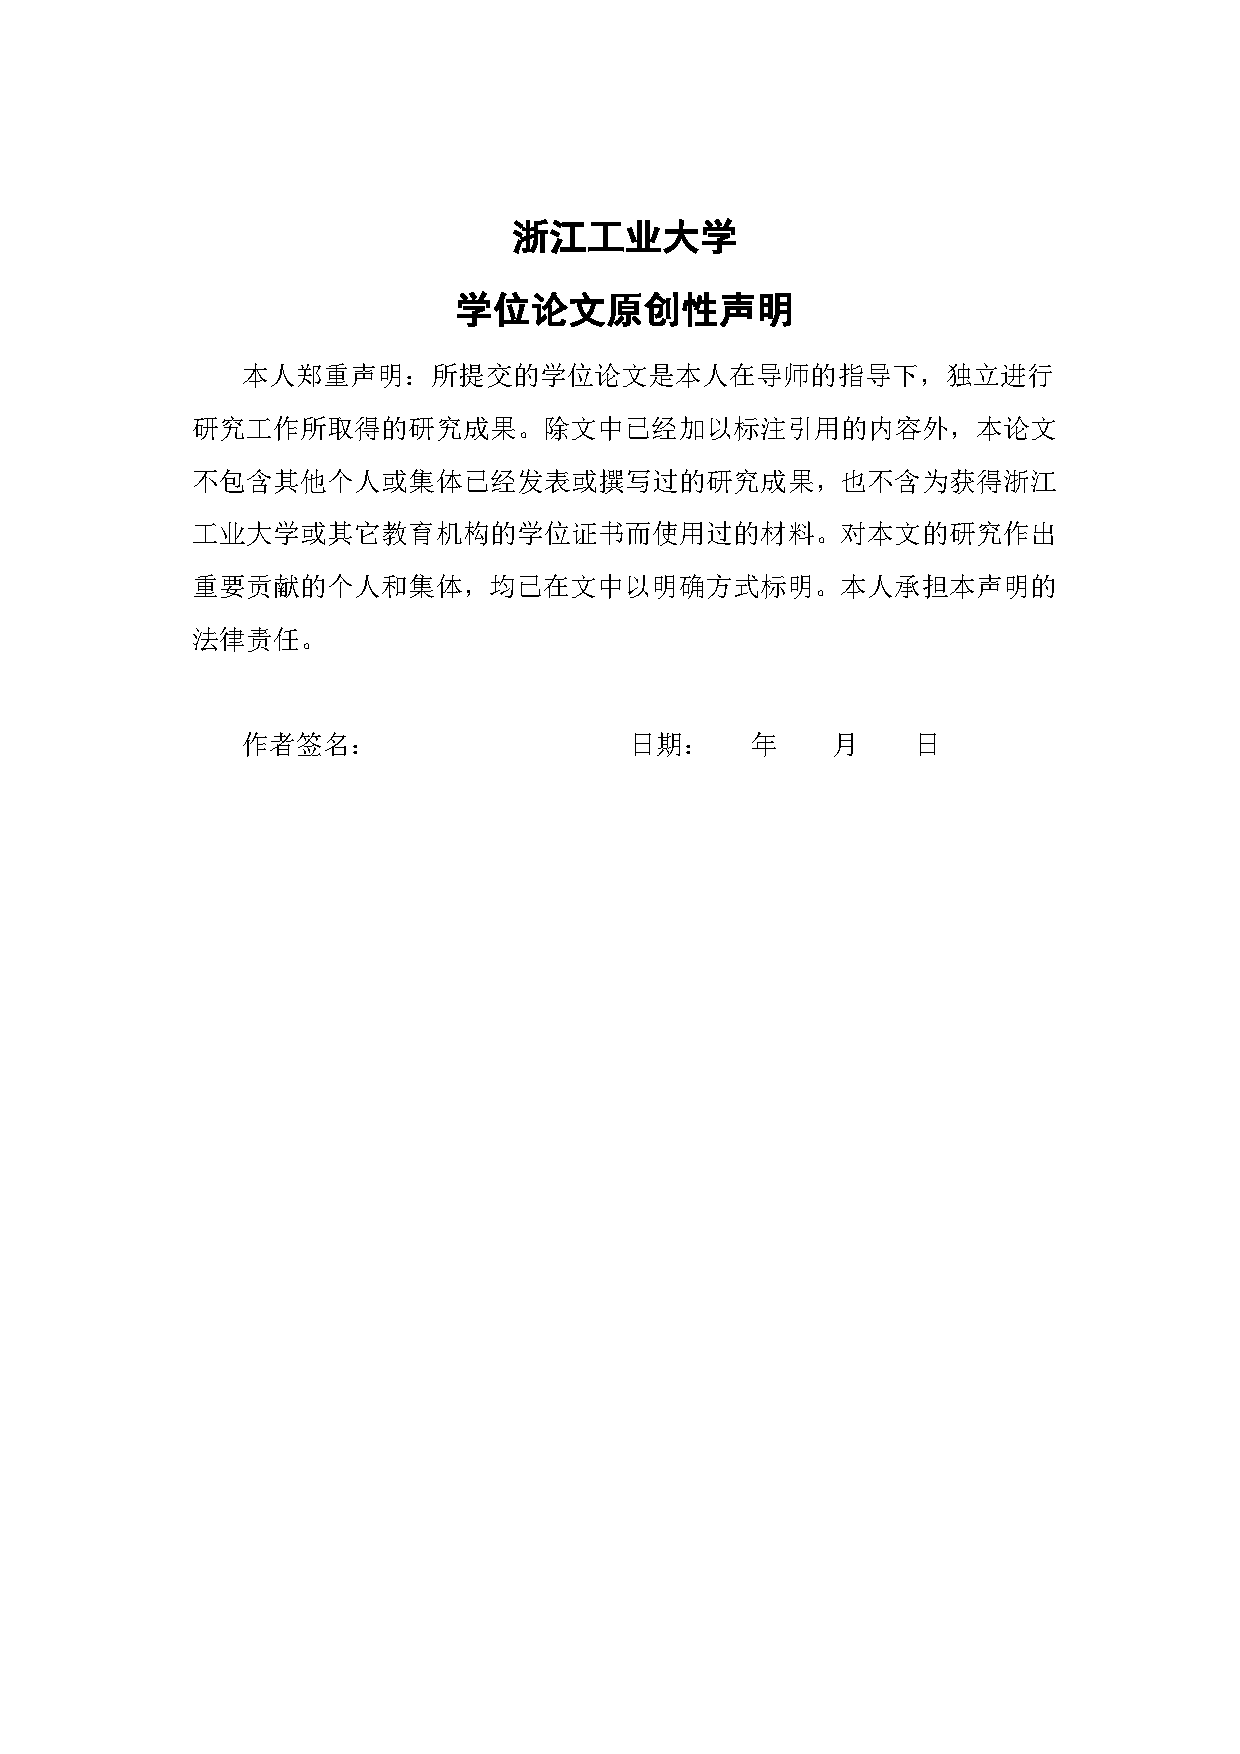
\includepdf{preface/statement}

%\listoffigures             % 图目录
%\pagenumbering{Roman}
%\listoftables              % 表目录
%\pagenumbering{Roman}


%%%%%%%%%% 正文 %%%%%%%%%%
%\mainmatter
\makeatletter
%\include{body/intros}
\begingroup % 在组内的chapter不换行
\let\clearpage\relax % chapter之后不换页
% !Mode:: "TeX:UTF-8"
% !TEX root = ..\paper.tex
\begin{abstractc}
\noindent \makebox[0pt][l]{\raisebox{8em}[0pt][0pt]{\songti\wuhao\bf 学号:\skyauthorid}}

\begin{center}
\vspace{-6mm}
{
\xiaosi

 学生姓名:\skyauthornamec\hspace{20mm} 指导老师:\skymentorc

\skyschoolc\skycollegec}
\end{center}
{\wuhao \songti \onequarterspacing
\noindent \textbf{摘要:}% !Mode:: "TeX:UTF-8"
本文针对某汽车电子零部件企业装配车间调度问题进行研究,该车间具有多条同质装配线,采用多品种、批量、面向主机厂的装配方式,存在提高产线利用率、降低冗余度、均衡生产等提升空间。突破主机厂限制是有效的解决方案,这是一个多品种多装配线轮番调度优化问题。

建立了$2$个调度优化模型,模型1 适用于订单到达稳定的情况,模型2 适用于不稳定的情况。两个模型都以加权拖延时间和与加权完成时刻和为主体,采用决策系数将之结合,模型2 需要考虑插单,引入和定义了产线闲置、流水线利用率、均衡率等概念以适应其情况,根据多品种和多流水线的特点,设计了相应的约束条件。在模型求解算法中,定义了虚拟序列的概念,将之与调度规则及启发式策略结合设计了交替改进(Cycle Amend, Cyc) 和虚拟序列(Virtual List, Vtr) 类多个求解算法。计算实验结果表明:Vtr -- Tabu 算法适用于中小规模的不考虑插单情况的问题,且随着工期目标的重视而凸显改进效果,VVT 算法的求解结果在多种不同决策环境下都显示出了较高的质量和稳定性。所提算法求解该模型是有效果的,所建模型也适合该问题。

本文所提的多品种多流水线轮番调度模型及其算法确实进一步提高了流水线利用率、按时交付等性能,仍存在如加入混流生产的改进空间。

\keywordsc{多品种多装配线,调度模型,虚拟序列,算法设计}
}
\end{abstractc}
\vspace{5mm}

\begin{abstracte}
\begin{center}
\vspace{1em}
{\xiaosi \onequarterspacing
 Author: \Skyauthorc\hspace{20mm} Mentor: \Skymentorc

\Skycollegec, \Skyschoolc

%{\xiaosan\bf\vbox{} Abstract}
}
\end{center}
{ 
\wuhao \onequarterspacing
\noindent \textbf{Abstract: } % !Mode:: "TeX:UTF-8"
Multi-type massive production usually takes part in the assembly line of electronic parts for auto-mobile, however, a myopic way that specialize assembly line by the main factories is widely used, so that low utilization , high redundancy and unbalance production always happens. A sound solution is to despecialize the assembly line, the implementation of this solution is a so called multi-type multi-assembly-line take-turn scheduling problem. In this study, 2 mathematical models is built for different levels of managenent to apply. With proposed concept of \textit{virtual list}, schedule rule and heuristic tactic, 5 algorithms: Cyc --ATC, Cyc -- ATCS, Cyc -- Tabu, Vtr -- Tabu, VVT in 2 classes are designed. Experiment takes with script in Python shows, that Vtr -- Tabu algorithm suits for small and median scale problem, especially for none-job-inseting high weighted date-related problem, while high stability and quality schedule in various aspects can be obtain with VVT algorithm.

\keywordse{~multi-type, multi-assembly-line, scheduling model, virtual list, algroithm design}}
\end{abstracte}

% !Mode:: "TeX:UTF-8"
% !TEX root = ..\Literature_Translation.tex
%%  绪论
\chapter{绪论}
\section{课题研究的背景和意义}
本文的研究对象是汽车零部件装配生产线,是典型的多品种小批量生产方式,并且在需求日益多样化的背景下,时常要根据产品调整生产。本文将从这种生产方式着手研究多品种产品的装配生产调度问题。

\subsection{课题研究背景}
汽车装配大多采用同步装配流水线方式作业,将装配过程分为多个作业单元,并安排在流水线的相应工位上,
车体在移到中装配,各工位同时作业。以往,汽车装配工厂固定地生产一种或少数几种车型,采用大批量、规模化的生产。然而,随着技术的日新月异,客户需求的多样化,以及精益思想、环保节能观念的出现,汽车工业的生产模式不得不转变为面向订单的小批量、多品种的生产方式。因此,缩短交货期、提高资源利用率、降低生产成本、提高生产运作的灵活性,已成为保证企业市场竞争力的重要手段。

多品种装配是在基本不改变或较少改变现有生产设施的前提下,通过对装配生产线的合理组织与调度优化,实现多品种共线装配,以最大限度地挖掘生产线的潜能,向客户提供定制的个性化产品和服务。

生产调度就是组织执行生产进度计划的工作,作为一种决策形式,调度在制造业扮演者至关重要的角色,尤其在现今充满竞争的环境下,有效的生产调度已成为能在市场竞争下生存的必须。

从上个世纪50年代起,调度问题的研究就受到应用数学、运筹学、工程技术等领域科学家的重视,科学家们利用运筹学中的线性规划、整数规划、目标规划、动态规划及决策分析方法,研究并解决了一系列有代表意义的调度和优化问题\cite{徐俊刚2004生产调度理论和方法研究综述}。

如今,随着计算机的发展,信息技术的成熟,许多过去只在理论层面上的调度算法,都可以通过计算机辅助得以验证与运用,给制造业的具体实力提升带来了可能。

\subsection{课题研究意义}
提高竞争力的方法有很多,对于汽车工业,产品需求多样化和市场细分化,促使越来越多的制造商将多品种装配作为增强其竞争能力的有效手段。具体来说,对于汽车零部件,装配过程主要是以零部件的安装、紧固为主,其次是联接、压装和加注冷却液、制动液等液体以及整车质量检测的工序,有时还要根据用户意向选装。因此,合理安排装配产线,优化调度作业单元,对保证汽车装配质量,快速响应需求,提高汽车装配线的生产效率有着重要的现实意义。

而实现多产品装配不仅需要技术上的支持,也需要有理论来实践。虽然在Henry Gantt 的那个时代起,调度的理论研究就受到了制造业的关注,然而生产模式的转变,信息技术的出现,都使得一些过去经典的调度算法不再适用,这就需要我们来修正那些方法,或者发展新的算法,本课题便是以此为中心。

举例来说,随着调度问题的规模增大,人们发现即使通过计算机,有些问题的算法并不是有效的,因为它们的求解超出了可接受的运行时间。逻辑学家和计算机科学家通过研究这类问题,建立了复杂度理论,并称这些问题是$NP$问题,问题的复杂度会是随着问题规模增大呈现指数爆炸。如果能从汽车行业的零部件装配调度出发,研究出通用的算法,那就间接证明了$P=NP$,可谓意义非凡。然而本课题重点不在此,这个问题对于作者来说难度太大。

这样一来,有时得到最优调度或者最优解的成本就变得太高了,那么近似最优解便成了很好的选择。然而调度问题的算法本来就众多,求解近似最优解更是如此,不同的算法适用的情况也不尽相同。因此,从多品种装配着手研究调度算法,对增加产品多样性,加快需求响应速度,加快提高企业的竞争力有着重要意义。

\section{课题研究的国内外现状}

你面向的对象是汽车零部件装配线  然后你的调度是有几个目标的 可以从对象和目标入手来写
同时也可以参考一些相关的硕士论文和博士论文 看他们的研究背景意义怎么写的
\subsection{国内研究状况}

\subsection{国外研究状况}
装配车间的生产调度决定了产品能否准时交货,某企业装配车间有多条装配线,每条装配线可分时轮番生产不同品种的产品,为了管理方便,按照产品所属厂家来安排组织生产,但这种方法存在负荷不均衡、换线损失等问题。课题对现在存在的问题进行分析,对所有需要生产的产品进行筛选组合,设计新的调度方案,以期获得均衡的生产线利用率、减少换线时间浪费、缩短完工时间、降低生产成本
% !Mode:: "TeX:UTF-8"
% !TEX root = ..\paper.tex
\chapter{多品种多装配线轮番装配调度优化模型}
某汽车电子有限公司主要产品为车用电子电器开关、控制模块、控制面板等,是美国通用、上海大众等国内外40余家汽车主机厂的专业定点配套供应商,该公司的订单特点是品种多、批量大、小型产品、工艺成熟,所以采用流水线生产是比较合适的,与其合作较多的客户(主机厂)一般有其专用线,专门负责该主机厂的订单生产。其专线生产策略带来诸如产能浪费严重,设备冗余等问题,需要突破流水线专用限制来进行改善。如此便是多品种多装配线的调度优化问题,需要进行建模求解。
\section{符号说明}

\section{基本假设}

% !Mode:: "TeX:UTF-8"
% !TEX root = ..\thesis.tex
\chapter{�㷨���}
��һ�¹�����4����Ʒ�ֲ�Ʒ���ȵ���ѧģ�ͣ���Ҫ������飬����Щģ�������NP--Hard���⣬��Ҫ�����Ӧ�㷨����⡣�����ģ��ǰ����Ҫ�Զ���(�ӵ�)����ʱ����㣬������Ҳ��ͨ���㷨�����⡣ģ�͵ľ�������㷨���Է�Ϊ�����ͺ͸Ľ��ͣ�ǰ�ߴ�û�е��ȵ������ʼ����һ�����ɹ����𽥰�����ҵ��ֱ������һ���Ϻõĵ��ȣ�����������ǰ�ߵĻ����ϣ��������е����Ը���Ŀ�ꡣ
\section{����ʱ�亯��}
\eqref{equ:processing}Ϊ����(�ӵ�)����ʱ�亯�����ɶ����ص����ҵ����ȷ������Ҫ�������˵�����£�\\[3pt]
\begin{supertabular}{ll}
$k$ & ��ҵ��ǣ�$k = 1,2,...,n_j$\\
$m_j$ & ����$j$�Ĵ�����Ԫ����\\
$i$ & ����$j$�Ĵ�����Ԫ��ǣ�$i = 1,2,...,m_j$\\
$q_{k,i}$ & ��ҵ$k$�ڴ�����Ԫ$i$�ϵĴ���ʱ��\\
$c_{k,i}$ &��ҵ$k$���ڴ�����Ԫ$i$�ϵ����ʱ��\\
$c_{j,\max}$ & ����$j$��������ҵ�������ڣ���$\max(c_k)$\\
\end{supertabular}\\[3pt]
���в�ͬ��ҵ��ͬ������Ԫ�ϵĴ���ʱ����ͬ�����Լ��Ϊ$q_i$��

���ڶ������ӵ�������ҵ�����IJ�𣬹ʿ��Ƕ�������������ƹ㵽�ӵ������ڣ���Ʒ���С�����Լ��账����Ԫ��Ļ���ռ��㹻�á�������ij����ˮ���ϵ���ҵ���Կ�������ˮ���价����û�л���ʱ�䣬���Ը�������Լ�Ϊ��$Fm\mid \mid C_{\max}$���Զ��׼����� $c_{j,\max} = c_{n_j,m_j}$�����������ѧģ�����£�
\begin{gather}
\min c_{n_j, m_j}\\[-2pt]
\text{s.t.}\notag
\end{gather}
\begin{numcases}{}
c_{1,1} = q_{1,1}\label{equ:processtime1}\\
c_{1,i} = \sum_{i=1}^{m_j} q_{1,i}\label{equ:processtime2}\\
c_{k,1} = c_{k-1,1} + q_{k,1} & $k = 2,3,...,n_j$\\
c_{k,i} = \max(c_{k-1,i} ,c_{k,i-1}) &$k = 2,3,...,n_j, i = 2,3,...,m_j$\\
q_{k,i}  = q_i & $k = 1,2,...,n_j, i = 1,2,...,m_j$
\end{numcases}

���������������ͼ����ʾ����ؼ�·����Ϊ�����ļ������̡���\ref{fig:directedgraph}��ʾ��ÿ���ڵ��ڱ�ʾ��ҵ�Ĵ���ʱ�䣬�����ʾ��ҵ����˳�������ʾ��ͬ�Ĵ�����Ԫ�������Ͻǿ�ʼ���������򻡵ķ������ڵ㣬��������½ڵ��ʱ�伴Ϊ��������ʱ�䡣
���У�\eqref{equ:processtime1}��(\ref{equ:processtime2})���Ի���õ������ʽ��$c_{k,1} = k\cdot q_1,(k = 1,2,...,n)$�����������㷨�ij�ʼ����
\begin{figure}[h]
\newcommand{\process}[1]{*++=[o][F]{\makebox[2em]{$#1$}}}
\begin{equation*}
\xymatrix{
\process{q_{1,1}} \ar[r] \ar[d] & \process{q_{1,2}} \ar[d] \ar[r] & \cdots\ar[r] & \process{q_{1,m_j}} \ar[d]\\
\process{q_{2,1}} \ar[r]\ar[d] & \process{q_{2,2}} \ar[d]\ar[r] & \cdots \ar[r] \ar[d]& \process{q_{2,m_j}} \ar[d] \\
\vdots\ar[d] & \vdots \ar[d]\ar[r] & \process{q_{k,i}}\ar[r]\ar[d] &\vdots \ar[d]\\
\process{q_{n_j,1}} \ar[r] & \process{q_{n_j,2}} \ar[r] & \cdots\ar[r] & \process{q_{n_j,m_j}}
}
\end{equation*}
\caption{��������ҵ��������ͼ\label{fig:directedgraph}}
\end{figure}

\newcounter{algor}%\newcounter{exam}
\theoremheaderfont{\heiti}
\newtheorem{algori}[algor]{�㷨}%\newtheorem{exam}[exam]{ʾ��}
\begin{algori}
����ʱ�亯�������㷨
\end{algori}

\begin{asparaenum}
\renewcommand{\labelenumi}{\bf Step\theenumi~}
\item ��ʼ����������ҵ����$n$�����账����Ԫ����$m$��Ȼ���������Ԫ����ʱ��$q_1,q_2,...,q_m$��
\item ����$c_{k,1} = k\cdot q_1,(k = 1,2,...,n)$����$i = 1$��
\item $i = i + 1, c_{1,i} = c_{1,i-1} + q_i$����$k = 1$��
\item $k = k + 1, c_{k,i} = \max(c_{k,i-1}, c_{k-1,i}) + q_i$��
\item ���$k<n$��ִ��\Step{3}������ִ��\Step{5}��
\item ���$i<m$��ִ��\Step{2}����������㷨��
\end{asparaenum}

\section{���ɹ���}
ǰ�����ᵽ��EDD�����FCFS�����dz����ĵ��ȷ��ɹ����ھ��������ҵ��ʱ��ͨ�����ȸ��ݷ��ɹ�����а��ţ����Է��ɹ��������ҵ���ŵij�ʼ���ԣ�Ȼ���پֲ��������ȷ����Խ�һ���Ż���һ������Ĺ�����ܵõ����ŵ��ȵij�ʼ�⣬��Ȼ���˾ֲ��������̣�Ȼ�������ܻ���Ҫ�޴��˼���ռ��ʱ��(����ö��)��ͬ��������ֱ���Ĺ��򽫻���������������Ѷȣ������ƶ����ɹ���ʱҪ��Ȩ�⡣
\subsection{��������}
\begin{asparaenum}
\item EDD(���罻����)
\suspend{asparaenum}

EDD����ӹ��ڽǶȳ���������ҵ���ս���ʱ�̵��Ⱥ�������򣬲������˳������������������ڲ��л�������һ��ij������Ԫ���У��Ϳ��Լ��̰��Ŷ����е��׸���ҵ����������������ڰ���Ŀ��͹�����صĵ�������
\resume{asparaenum}
\item WSPT(��Ȩ��̴���ʱ��)
\suspend{asparaenum}

WSPT������SPT(��̴���ʱ��)�����һ�㻯������ҵ�Ĵ���ʱ������������깤ʱ��ΪĿ��ĵ��������Ϊ���ʡ�������򽫴�����ҵ����$w_j/p_j$ֵ������˳�����У�����ʱ��ϳ�����ҵ�������ڽϺ��λ�ã���һ���̶��ϼ������Ŷӵȴ�ʱ�䣬���ҿ���֤��WSPT�����$1\mid \mid \sum w_jC_j$�ĵ��������ŵ�\cite{pinedo}��Ȼ����$Pm \mid \mid \sum w_jC_j$ �����²���һ�������š�

\resume{asparaenum}
\item MS(��С�ɳ�)
\end{asparaenum}

MS����ͨ��������ҵ�Ľ��ȳ̶���������ҵ���ȣ���ǰ���������������ڣ���������Ƕ�̬�ģ�����ϵͳʱ��$t$��ء���ҵ����$\max (d_j - p_j - t , 0)$��ֵ�Ǽ���˳�����У���Ȼ��Ϊ���ȵ���ҵ�ᱻ������ǰ�棬���Ҳ�ͬ��ϵͳʱ���Ӱ�����е�˳�򣬳��ֶ�̬�ĵ��ȡ��ù��������ڰ���Ŀ��͹�����صĵ�������
\subsection{���Ϲ���}
���Ϸ��ɹ������ۺ���������������һ������ʽ������������������Եı�������������ȷ���������Է��Ϲ���Ӱ��̶ȵı�����û�й̶�����ʽ����������һ����ATC(�����ͺ�ɱ�)����

ATC�����ۺ���WSPT�����MS����ÿ���п��д�����Ԫʱ�����д�������ҵ��\eqref{equ:orderindexexample}����������ָ����ѡ���������ָ��ֵ����ҵ���д�����
\begin{equation}
I_j(t) = \frac{w_j}{p_j}\exp\left(-\frac{\max(d_j - p_j - t, 0)}{K\bar p}\right) \label{equ:orderindexexample}
\end{equation}
ʽ�У�

\begin{tabular}{ll}
$K$ & �����������\\
$\bar p$ &ʣ����ҵƽ������ʱ��
\end{tabular}

���Կ�����$K \to \infty$ʱ��$I_j(t) \to w_j/p_j$����ʱATC�����ת��ΪWSPT���򡣵�$K \to 0$ʱ������ҵ$j$���������ڣ���$\max(d_j - p_j -t , 0 ) = 0$����ôATC����Ҳת��ΪWSPT��������ҵ����������ڣ�����$d_j - p_j - t$��Ӱ�쳬��$w_j/p_j$������ATC��ת��ΪMS����ATC������Խ����׵�Ӧ�õ�$Pm\mid\mid \sum w_jT_j$���⣬��ؼ��������ڱ�������$K$��ѡȡ��

\section{����ģ��}
����ģ������ҪĿ�꺯��\eqref{equ:objmain}����ҪĿ�꺯��\eqref{equ:objsecond}��Լ������\eqref{equ:basicst1} -- (\ref{equ:basicst7})��ɣ������ŵ��ȵ���������ʼ���н����ĸĽ����ֱ��ڹ����ͺ͸Ľ����㷨��������
\subsection{�����㷨}
�����㷨����Ҫ������ȷ�����ɹ�����Ȼ���ܱ�֤�õ����ŵ��ȣ���ȴ���źܸߵ�ִ���ԣ����ڼƻ����š�����ģ�͵���ҪĿ��Ϊ��Ȩʱ�ӳټ��ܺͣ����Բ���ATC��������Ҫѡȡ�ʵ��ı�����������$C_{\max} = \max(C_j)$��Ϊ���е�����ҵ��������ʱ�̣��ڵ���ȷ��ǰ���������Ǽ򵥹��ƣ�
\[
\hat{C}_{\max} = \sum_{j = 1}^n p_j + n\bar s
\]
ʽ�У�$\bar s $Ϊʣ����ҵ��ƽ��׼��ʱ�䡣
���巶Χ���ӿ�Ϊ��
\[
R = \frac{d_{\max} - d_{\min}}{C_{\max}}
\]
һ�����\eqref{equ:proporpara}��ȷ������������

\begin{equation}
K = 
\begin{cases}
4.5 + R , & R\le 0.5\\
6 - 2R , &R >0.5 \label{equ:proporpara}
\end{cases}
\end{equation}

��Ի���ģ�͵�ʵ������������е���ҵΪ���������������ϴ���ʱ����Ϊ�������Ĵ���ʱ�䣬Ϊ�˷�����������㷨����

\begin{algori}
����ģ��ATC������ȹ����㷨
\end{algori}

\begin{asparaenum}
\renewcommand{\labelenumi}{\bf Step\theenumi~}
\item ��ʼ����$J = N$,
\end{asparaenum}

\subsection{�Ľ��㷨}

\section{�嵥ģ��}
\subsection{�����㷨}

\subsection{�Ľ��㷨}
\section{�ֵ�ģ��}
\subsection{�����㷨}

\subsection{�Ľ��㷨}
\section{�ۺ�ģ��}
\subsection{�����㷨}

\subsection{�Ľ��㷨}

\section{��}

% !Mode:: "TeX:UTF-8"
% !TEX root = ..\thesis.tex
\chapter{计算实验及算法评估}
本章将对上一章的算法进行评估,通过设计相关计算实验,建立评价体系,具体评估各算法的效果及其适用规模。然后根据实验结果,为研究对象制定合适的调度方案。
\section{算法评价体系}

到达时间:Poisson分布
处理时间:负指数分布(指数分布)、艾尔朗分布

由\reft{tab:2jobshopinfo},流水线的数量可以是$5,6,7$,产品品种的范围是$29\~ 777$,所以合理的作业数量为$30,50,100,200,500,1000$
,作业处理时间单位为转换过的 $t.u.$,由于每个订单的作业批量都比较大,所以订单处理时间单位为$500 t.u.$
产品特点是体积小,而每个订单所含的产品数量,即需要考虑的作业数量大,一般在$1000\~ 2000$左右
\section{实验设计}
\lstset{	basicstyle = \small\ttfamily,
	keywordstyle = \color{blue}\bfseries,
	stringstyle = \color{red},
	emph = {solve},
	emphstyle = \color{Green}\bfseries,
	commentstyle = \color{CadetBlue}
	}
\begin{lstlisting}[language = Python]
def solve(input_data):
	data = input_data.split('\n')		# load data
	n = len(data)		
	N = range(n)



import sys
if __name__ == '__main__':
	if len(sys.argv) > 1:
		file_location = sys.argv[1].strip()
		output = sys.argv[2].strip()
		input_data_file = open(file_location, 'r')
		input_data = ''.join(input_data_file.readlines())
		input_data_file.close()
		solve(input_data)


\end{lstlisting}

\section{结果及评估}


\section{小结}
% !Mode:: "TeX:UTF-8"
\chapter{总结}



\bibliography{references/reference}
\makeatother
%\backmatter
\endgroup % 组结束
\clearpage % 显式换页,使书签定位准确


%%%%%%%%%% 参考文献 %%%%%%%%%%

%\nocite{*}   % 若将此命令屏蔽掉,则未引用的文献不会出现在文后的参考文献中。

%%%%%%%%%% 致谢 %%%%%%%%%%
%% !Mode:: "TeX:UTF-8"

\chapter{\acknowledgementtitle}

浙江工业大学本科生毕业论文~\LaTeX~模板主要参考以下内容:
\begin{itemize}
  \item 天津大学本科生毕业论文
  \item 哈尔滨工业大学~PlutoThesis~硕博士学位论文模板
  \item 武汉理工大学学位论文~WHUTThesis~模板
  \item 中科院~CASthesis~模板
  \item 浙江大学~cs\_zju\_theis~模板
  \item 上海交通大学毕业论文Latex模板
\end{itemize}

\vspace*{1em}

衷心感谢导师~XXX~(职称)对本人的精心指导。他/她的言传身教将使我终生受益。

感谢~XXX~教授,以及实验室全体老师和同窗们的热情帮助和支持!




            % 致谢
%\include{body/lit}
%%%%%%%%%% 附录 %%%%%%%%%%
%\appendix
%% !Mode:: "TeX:UTF-8"
% !TEX root = ..\thesis.tex
\chapter{实验结果图表}
模型1 和模型2 运用其相应的不同算法得到了目标函数值、流水线均衡率等结果,图表可以让不同算法的对比显得直观。不同决策参数$\lambda_1$、流水线数量$m$及订单数量$n$的环境下,模型1 的所得结果如\reff{fig:result1} -- \reff{fig:result3}所示,模型2 的所得结果如\reff{fig:result4} -- \reff{fig:result9}所示。
\begin{sidewaysfigure}
\centering
\subfloat[$n = 20$]{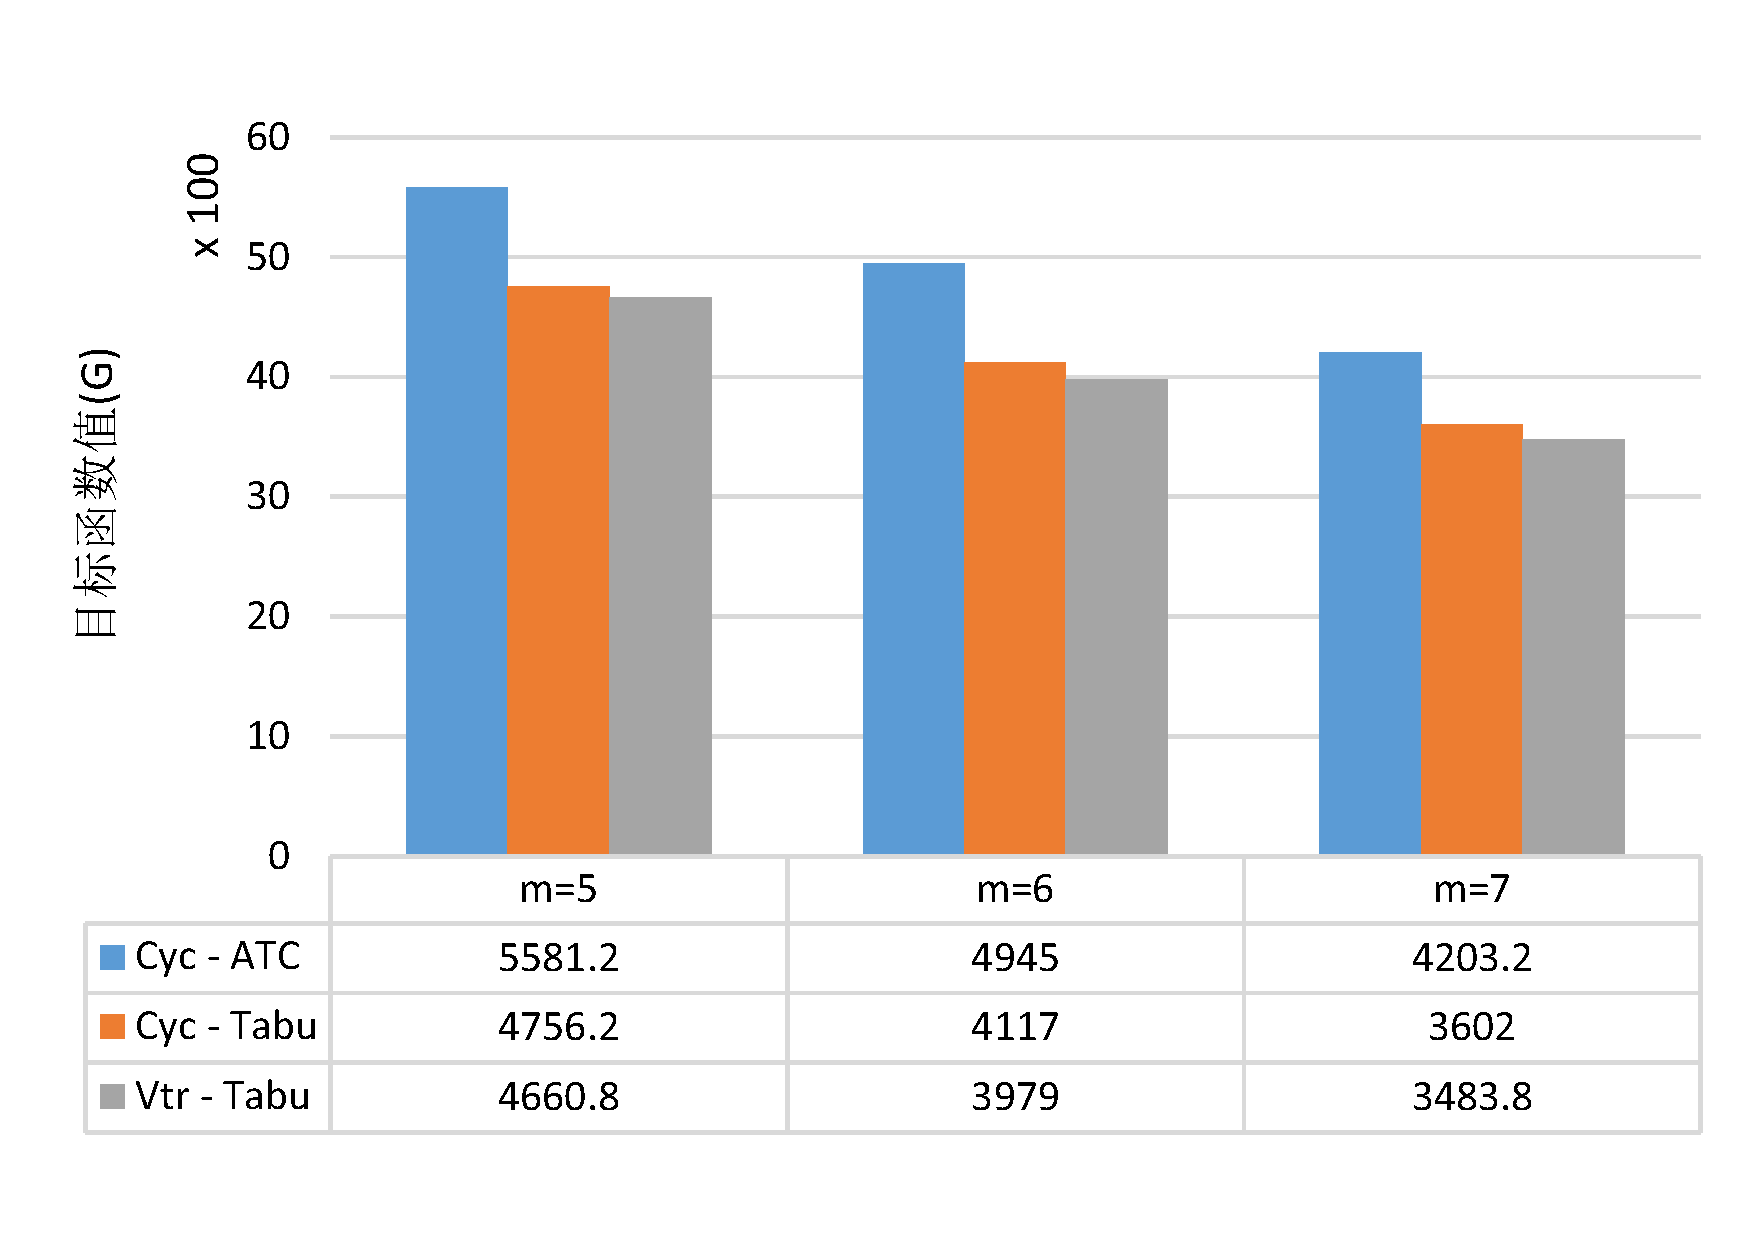
\includegraphics[height = 6cm, angle = -90]{basic_04_20}}
\subfloat[$n = 30$]{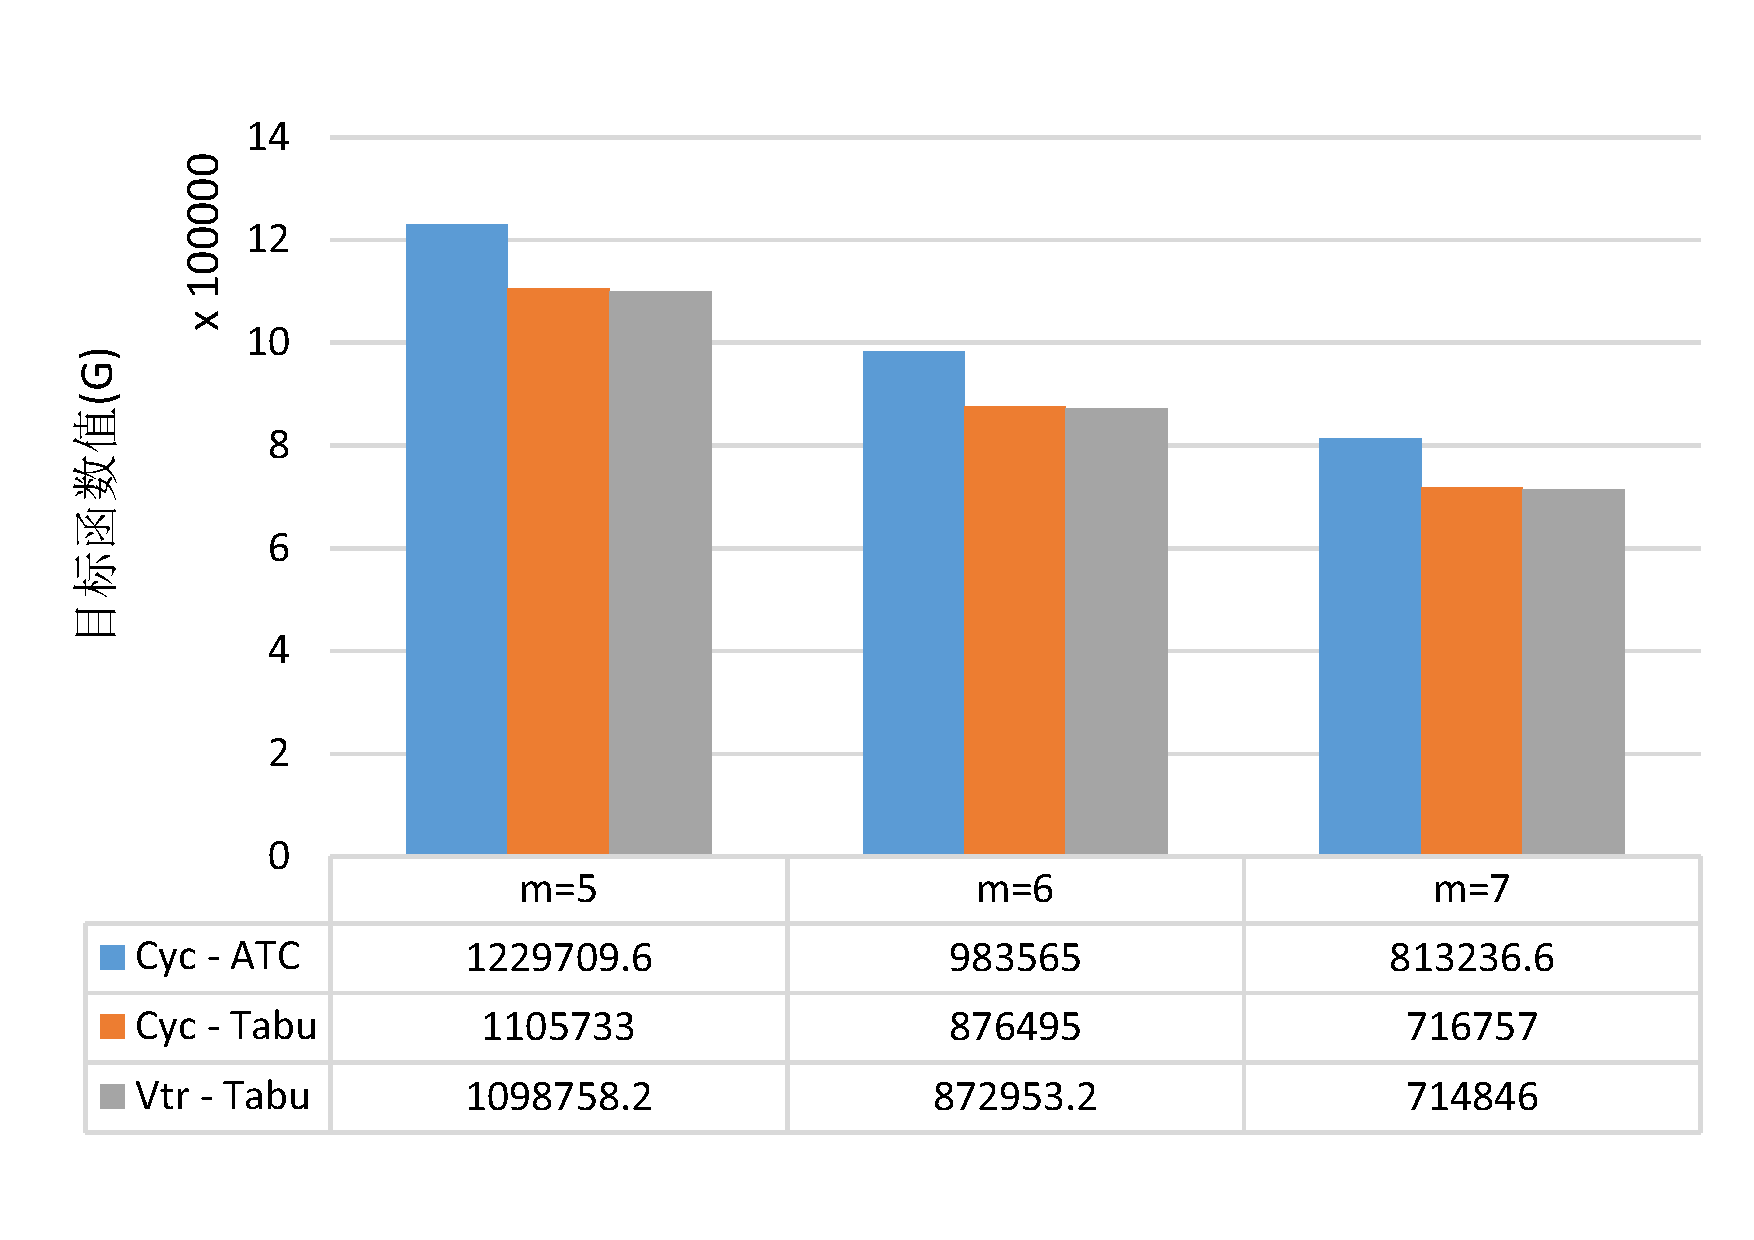
\includegraphics[height = 6cm, angle = -90]{basic_04_300}}
\subfloat[$n = 50$]{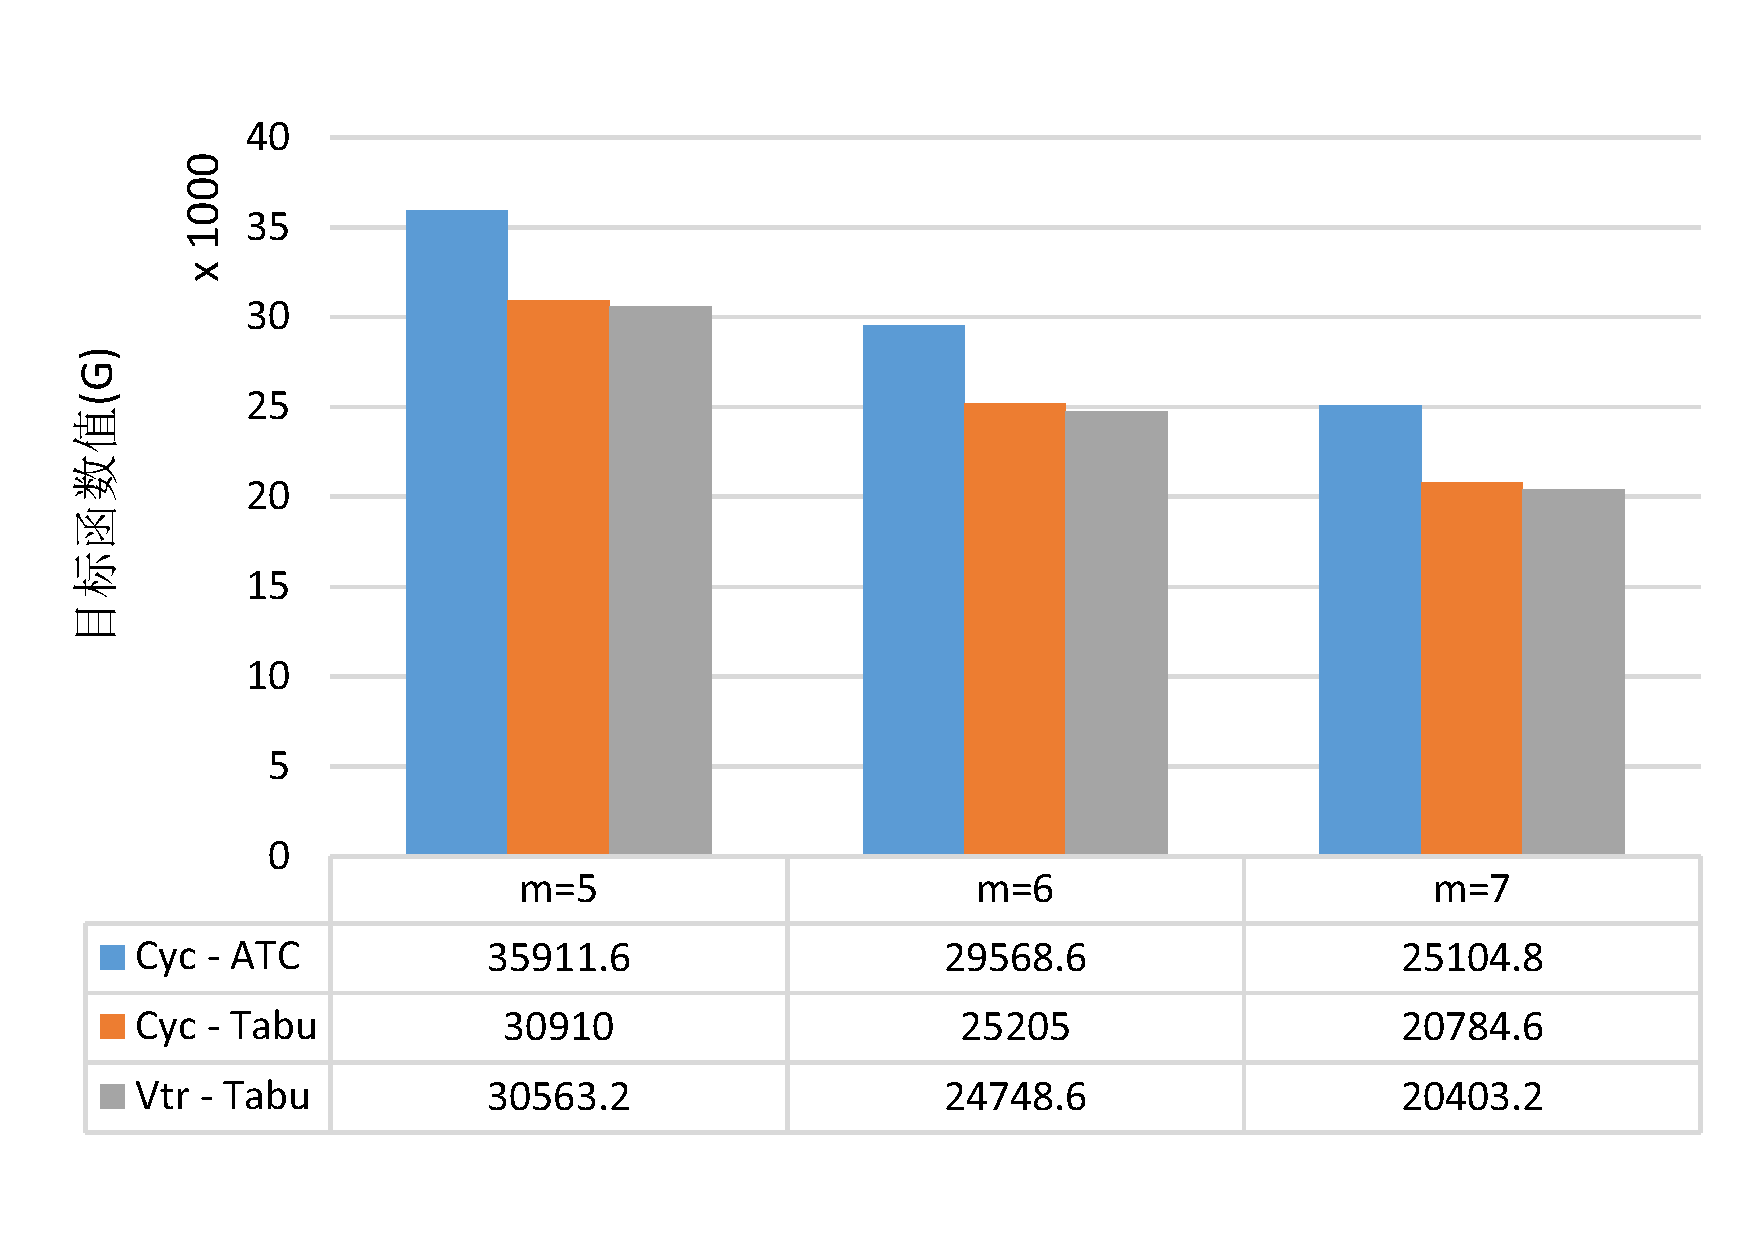
\includegraphics[height = 6cm, angle = -90]{basic_04_50}}
\subfloat[$n = 70$]{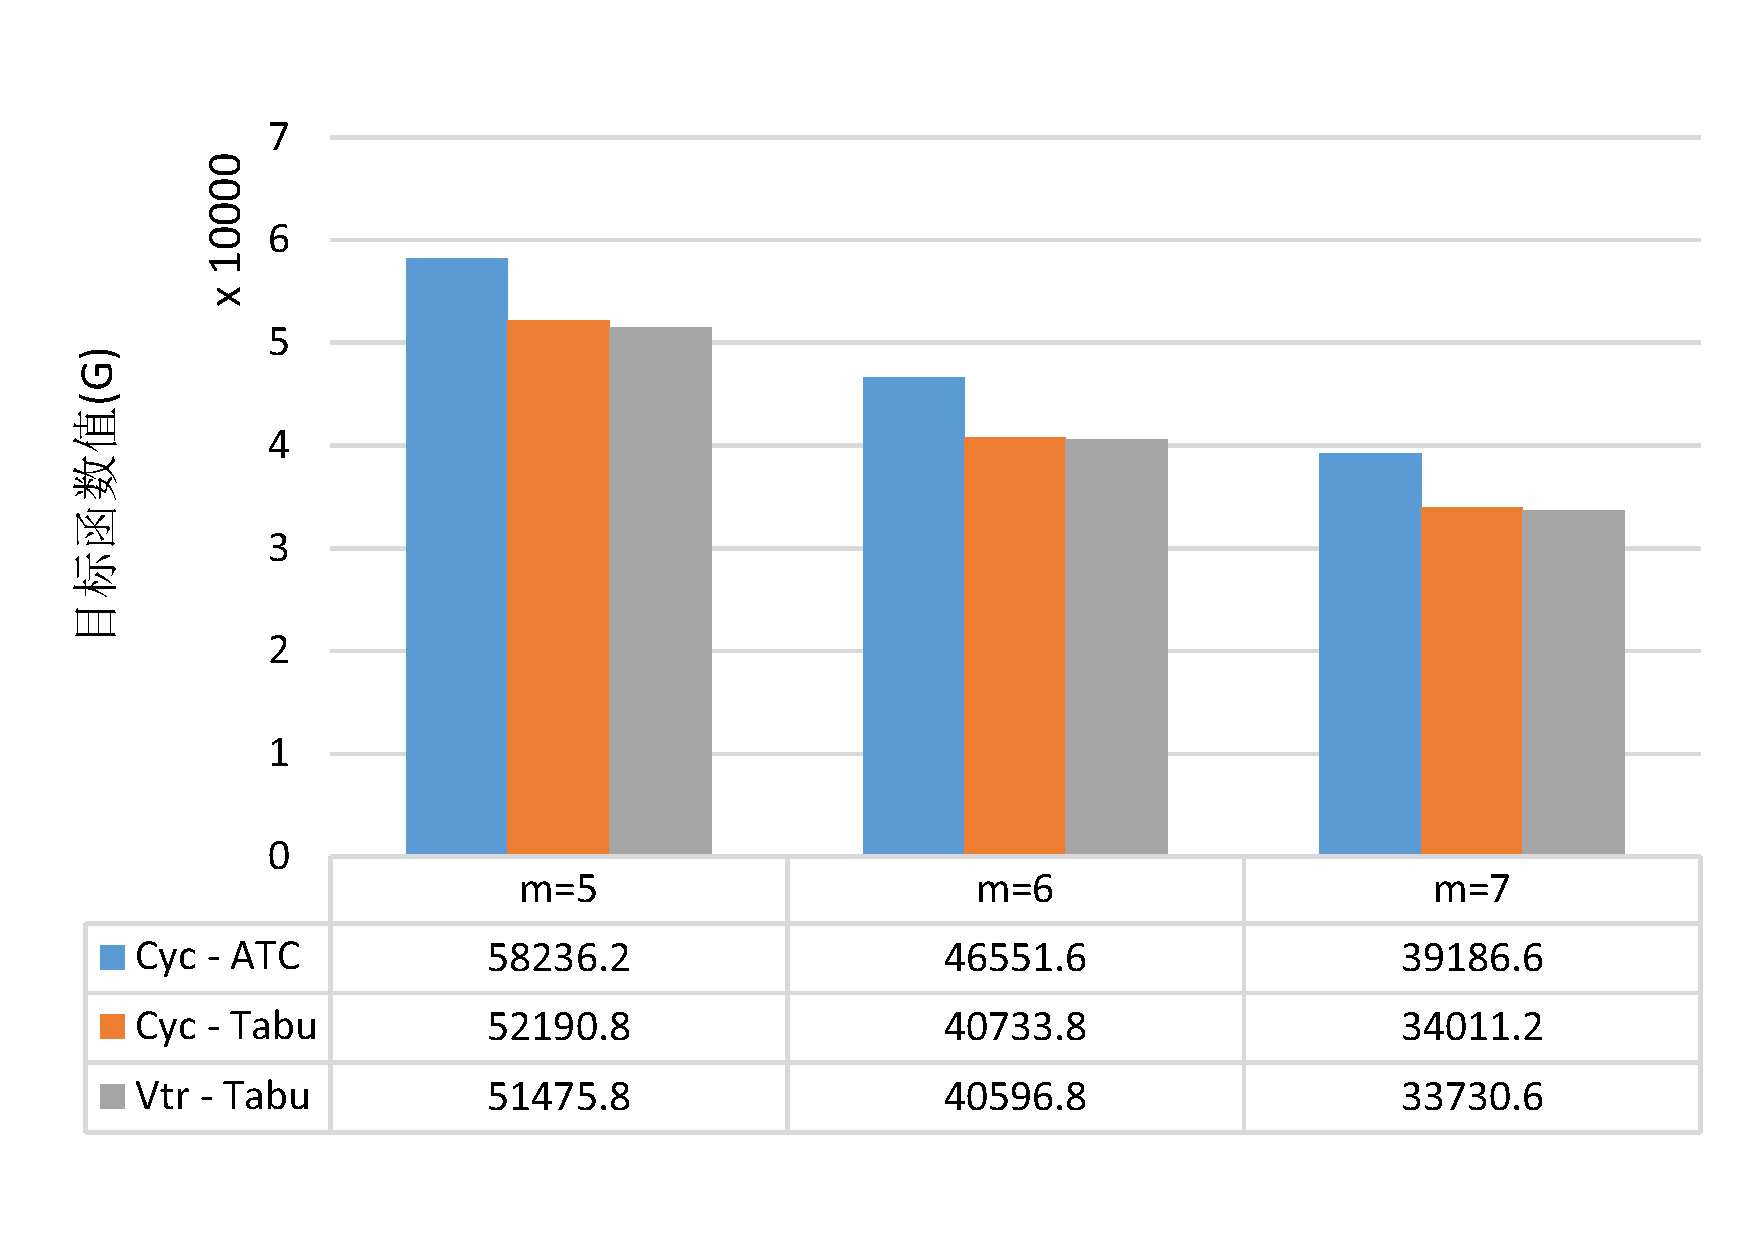
\includegraphics[height = 6cm, angle = -90]{basic_04_70}}\\
\subfloat[$n = 100$]{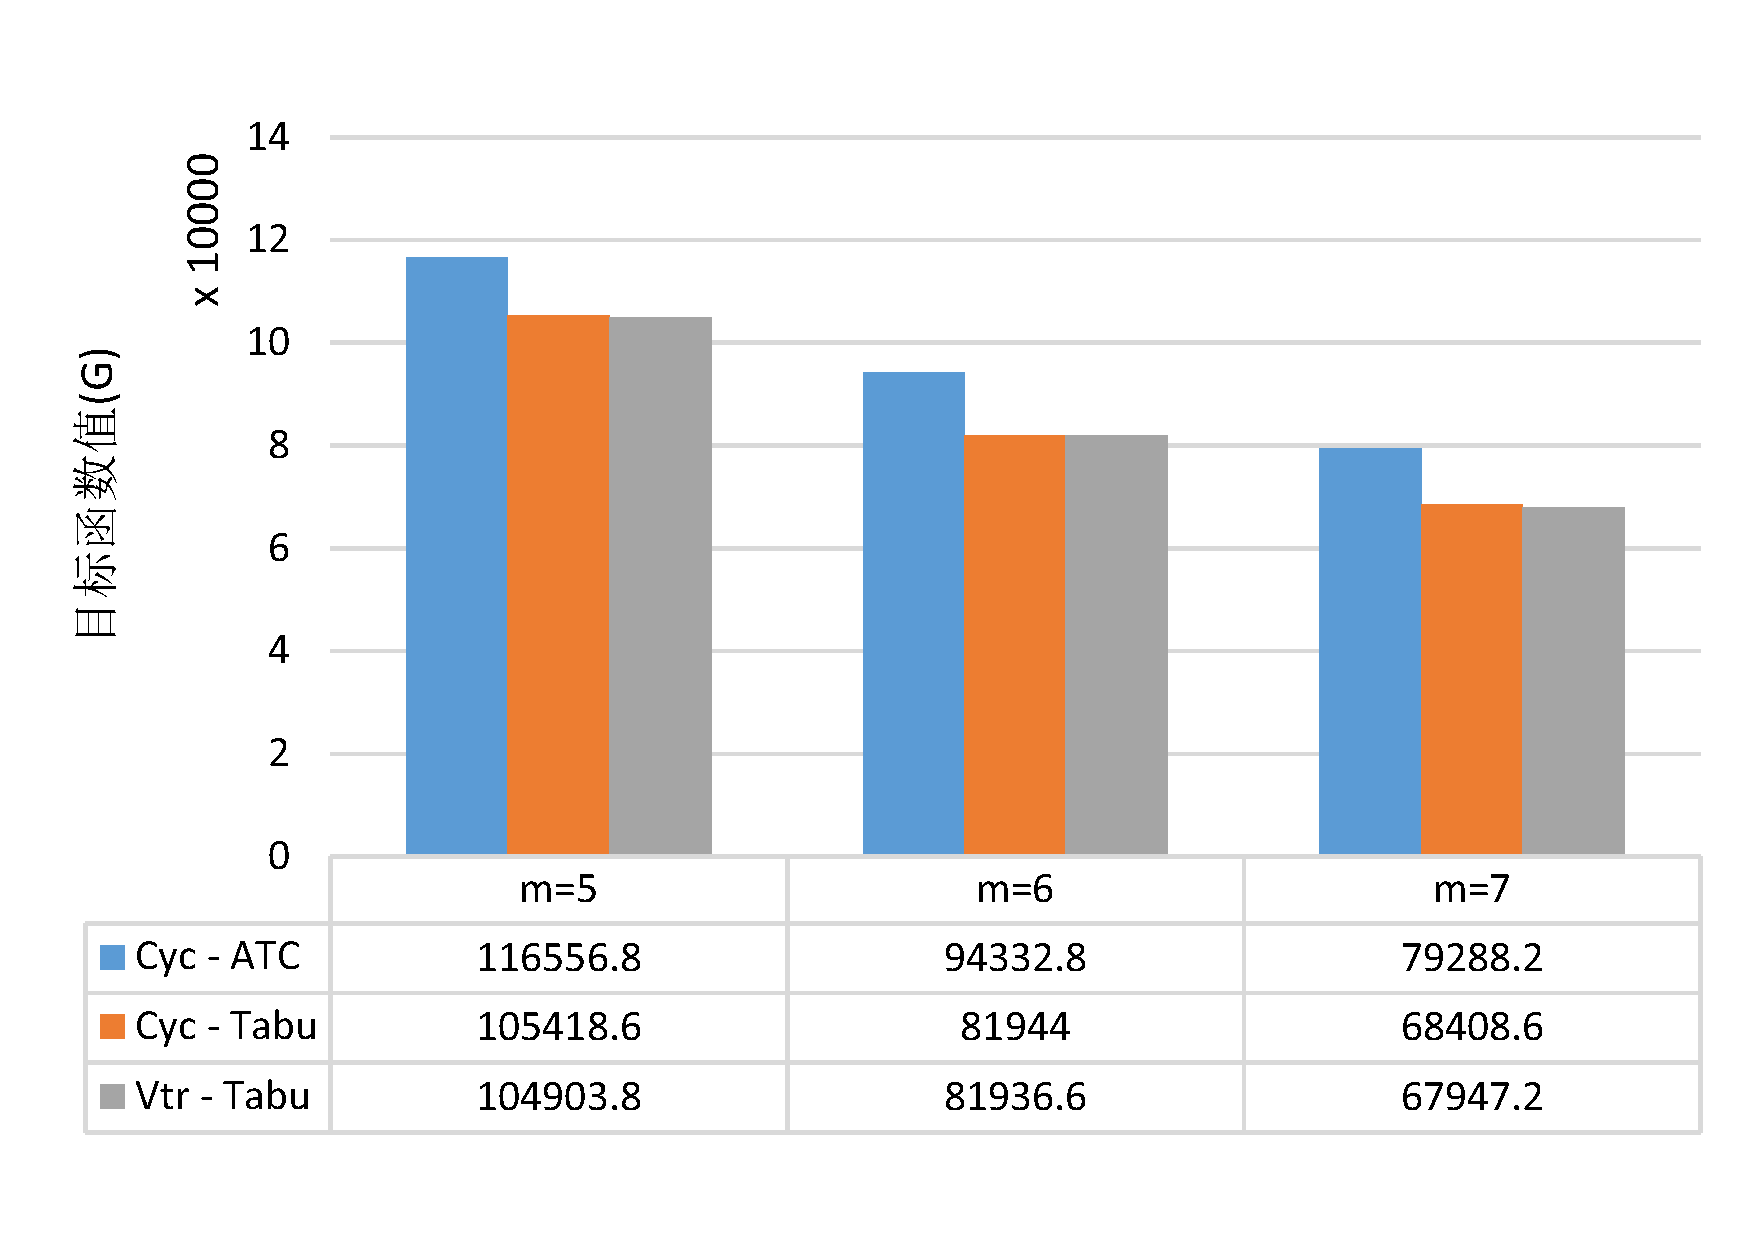
\includegraphics[height = 6cm, angle = -90]{basic_04_100}}
\subfloat[$n = 150$]{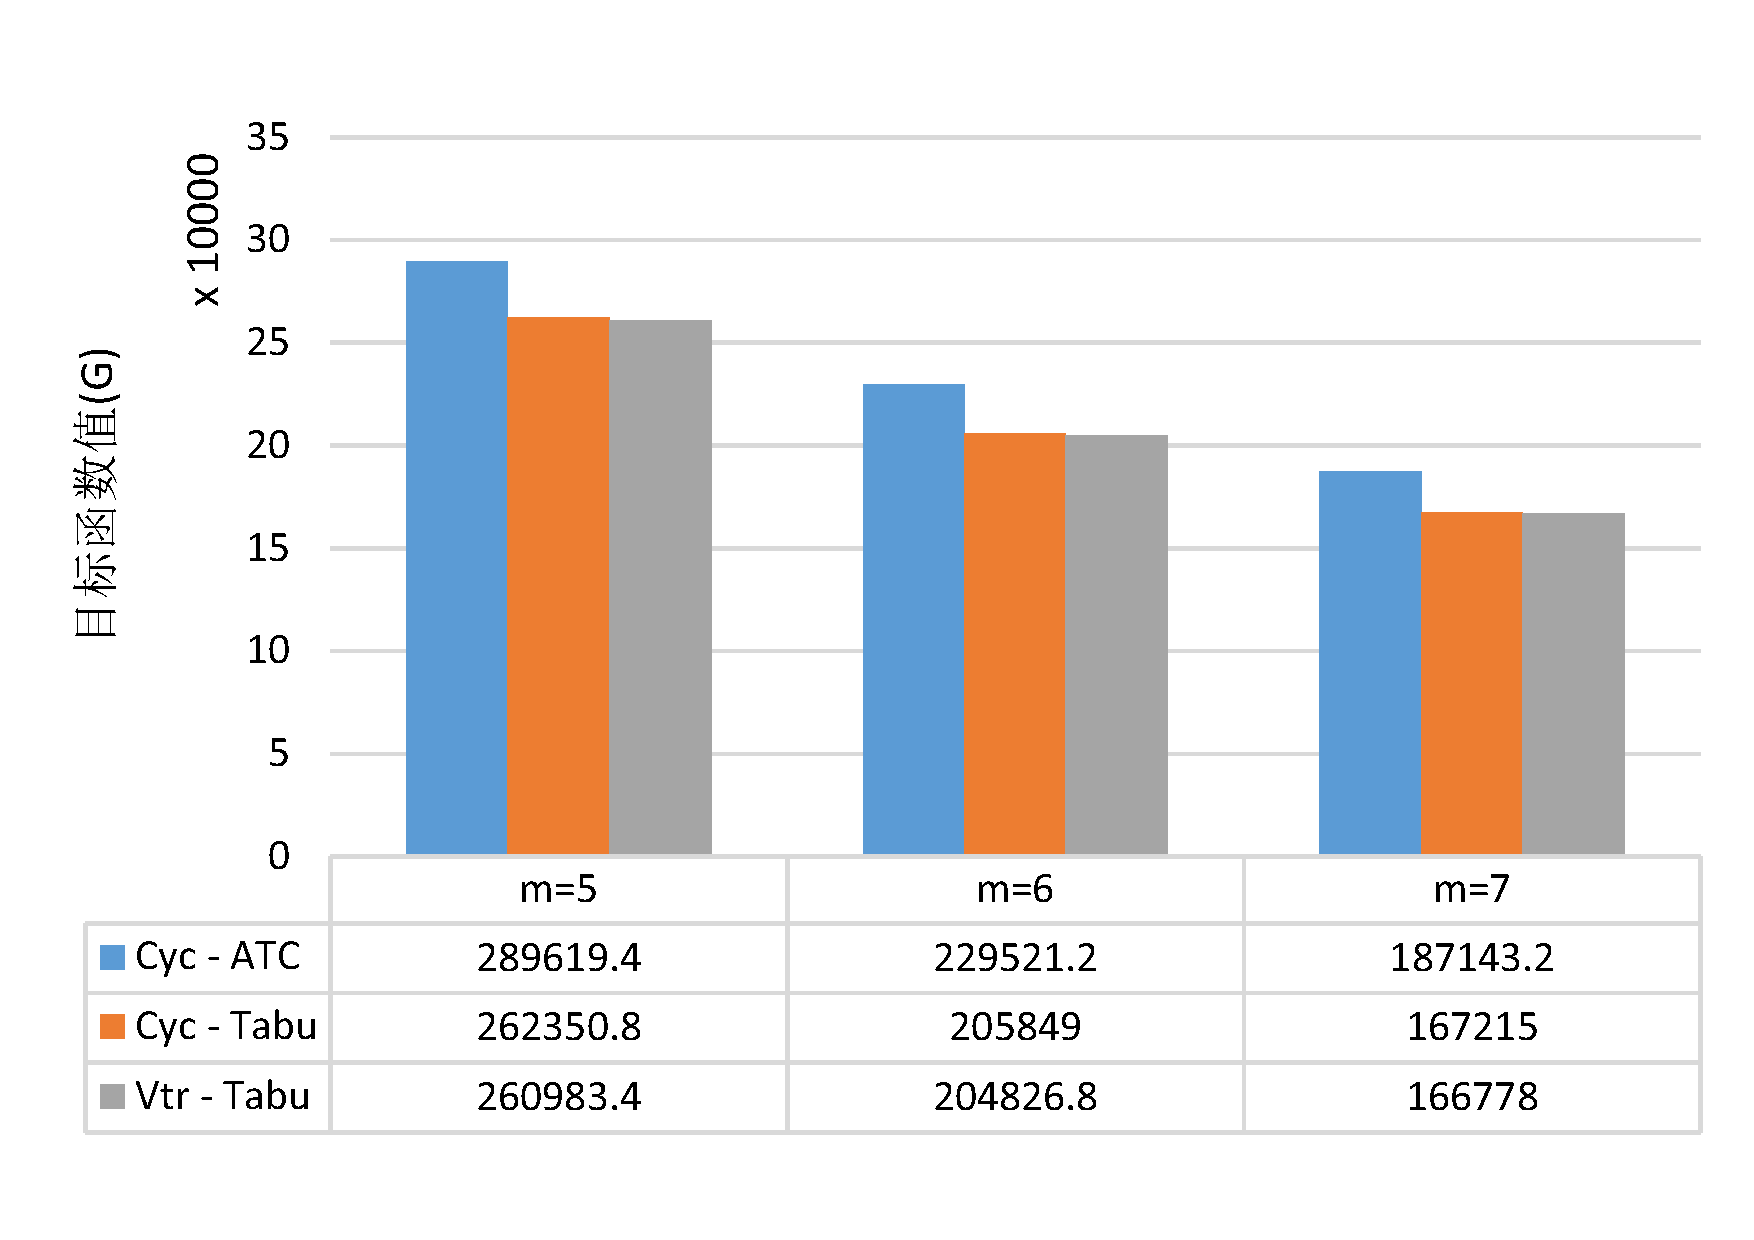
\includegraphics[height = 6cm, angle = -90]{basic_04_150}}
\subfloat[$n = 200$]{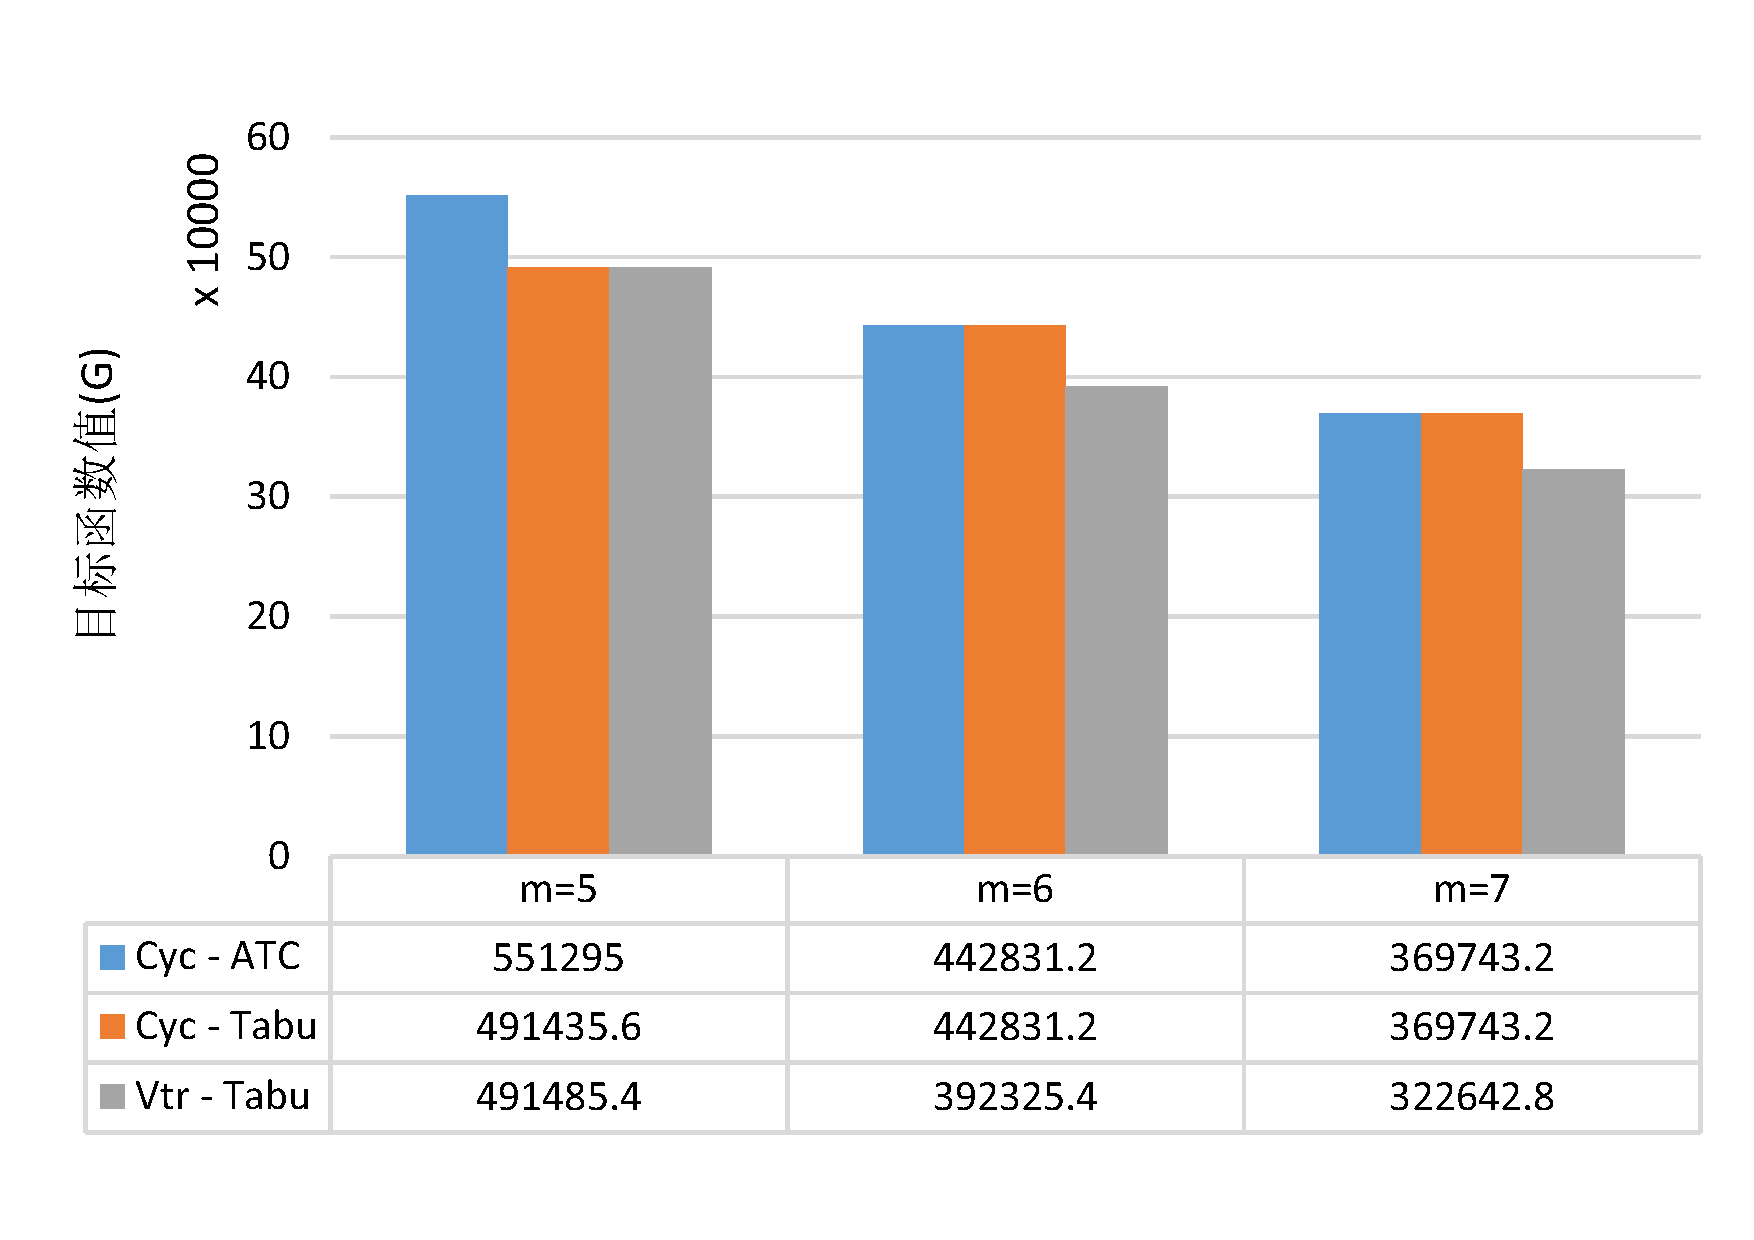
\includegraphics[height = 6cm, angle = -90]{basic_04_200}}
\subfloat[$n = 300$]{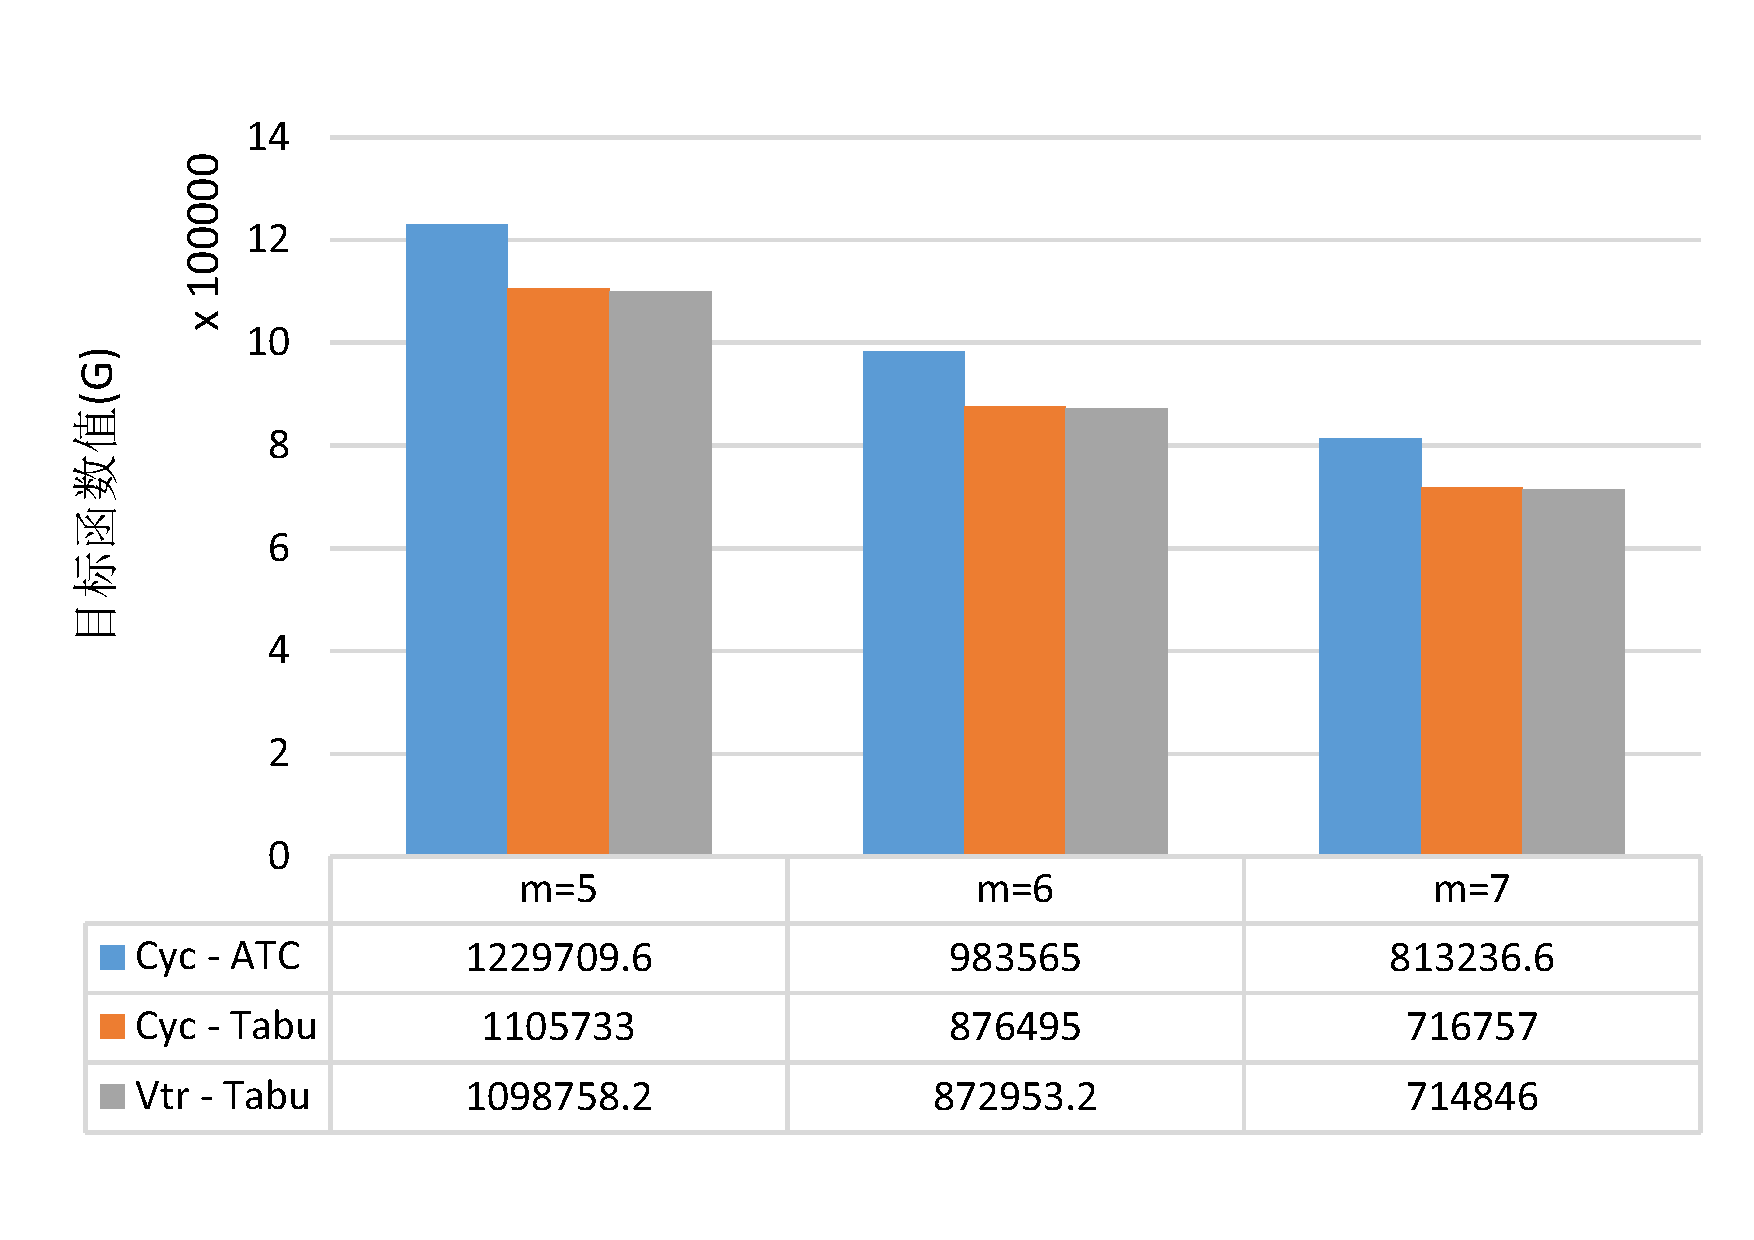
\includegraphics[height = 6cm, angle = -90]{basic_04_300}}\\
\subfloat[$n = 500$]{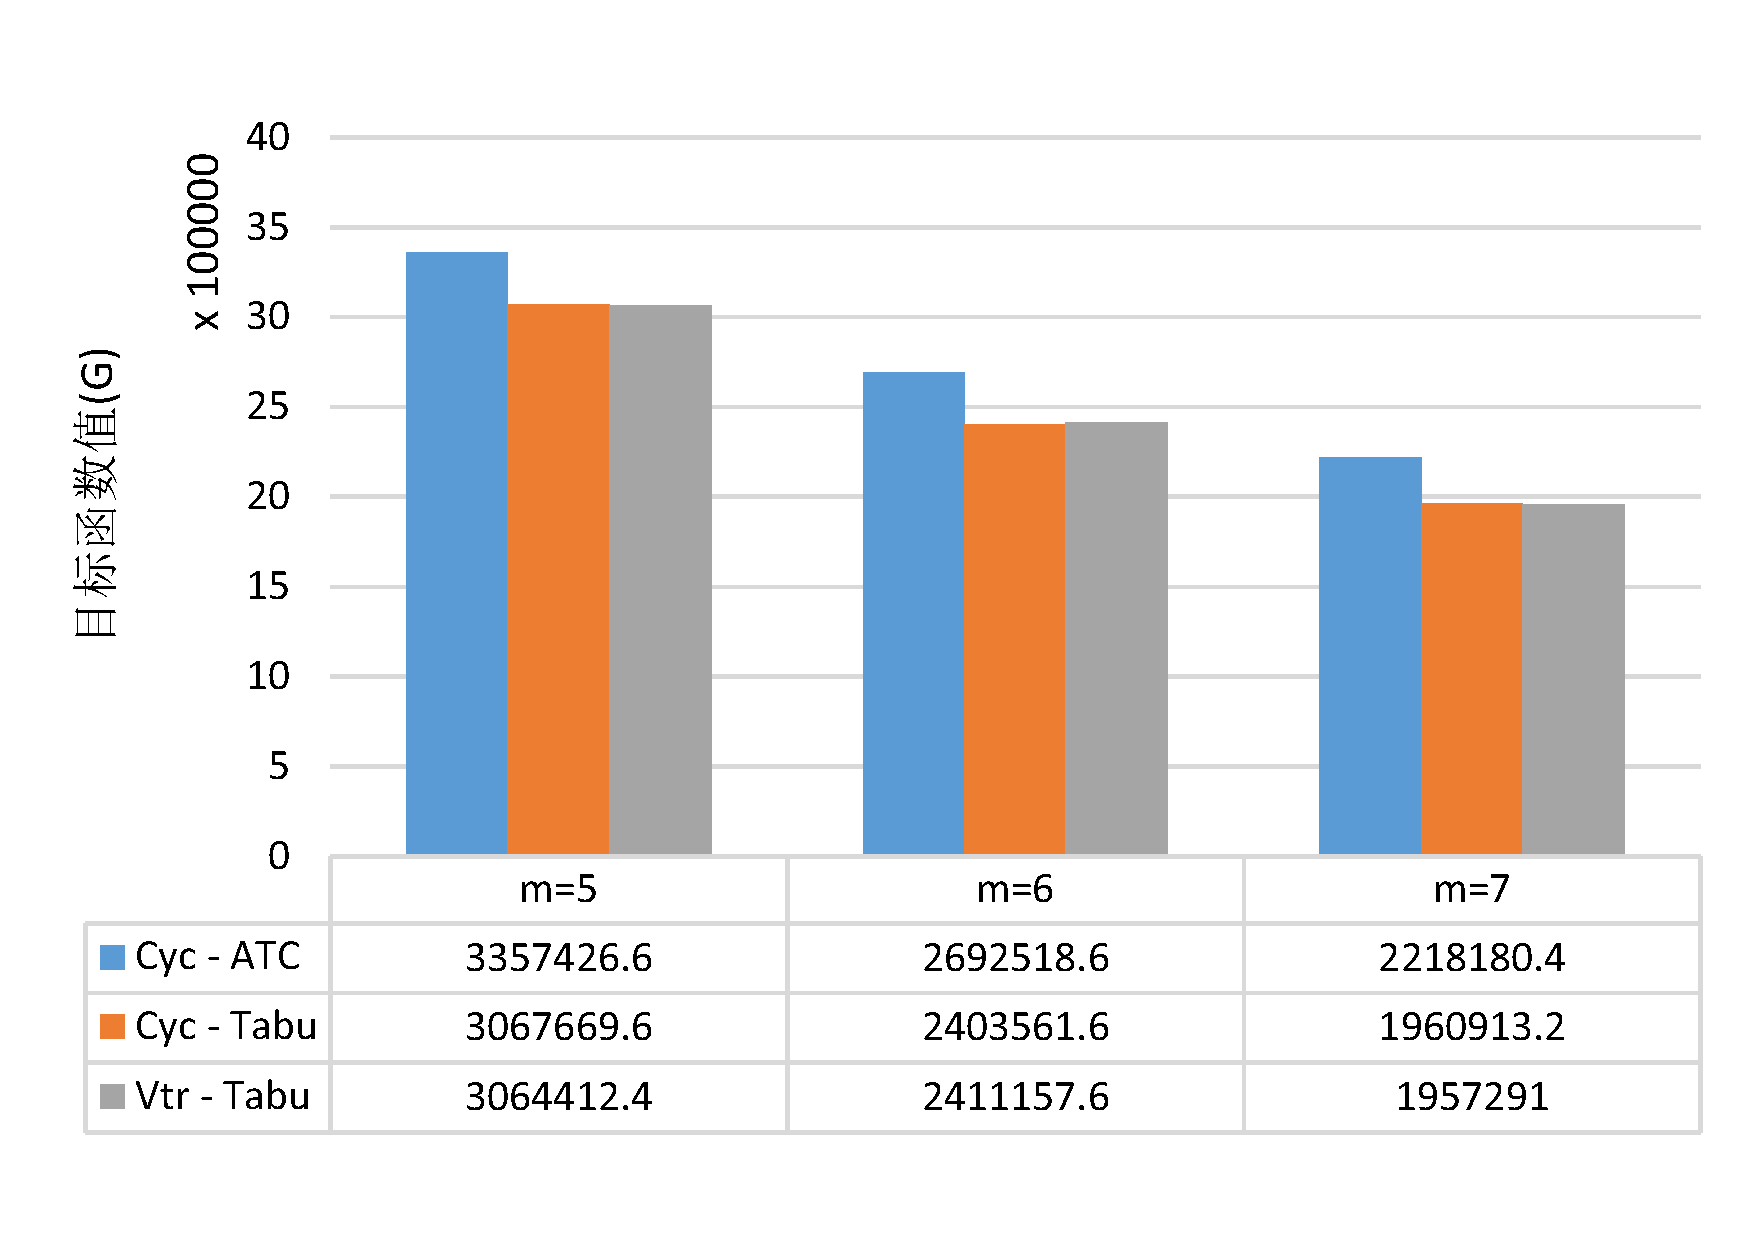
\includegraphics[height = 6cm, angle = -90]{basic_04_500}}
\subfloat[$n = 750$]{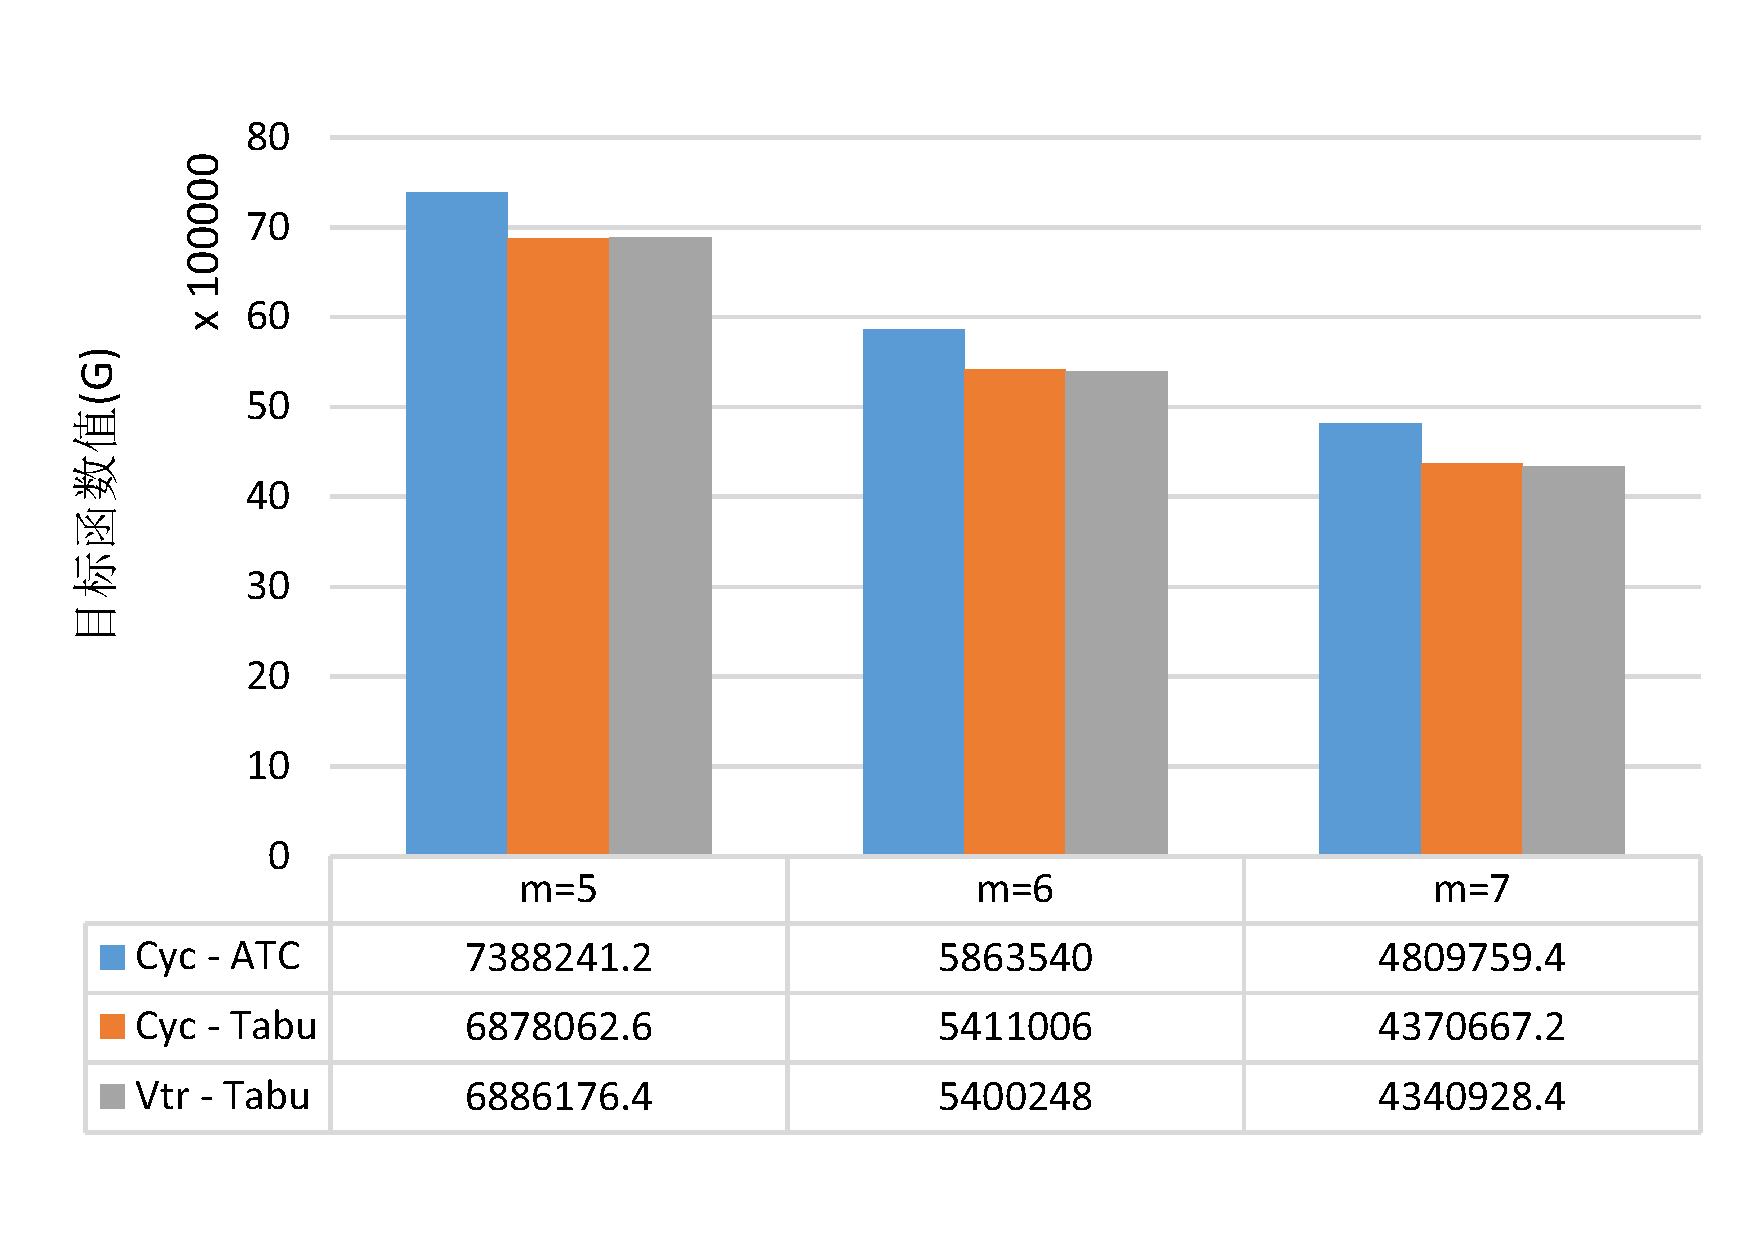
\includegraphics[height = 6cm, angle = -90]{basic_04_750}}
\subfloat[$n = 1000$]{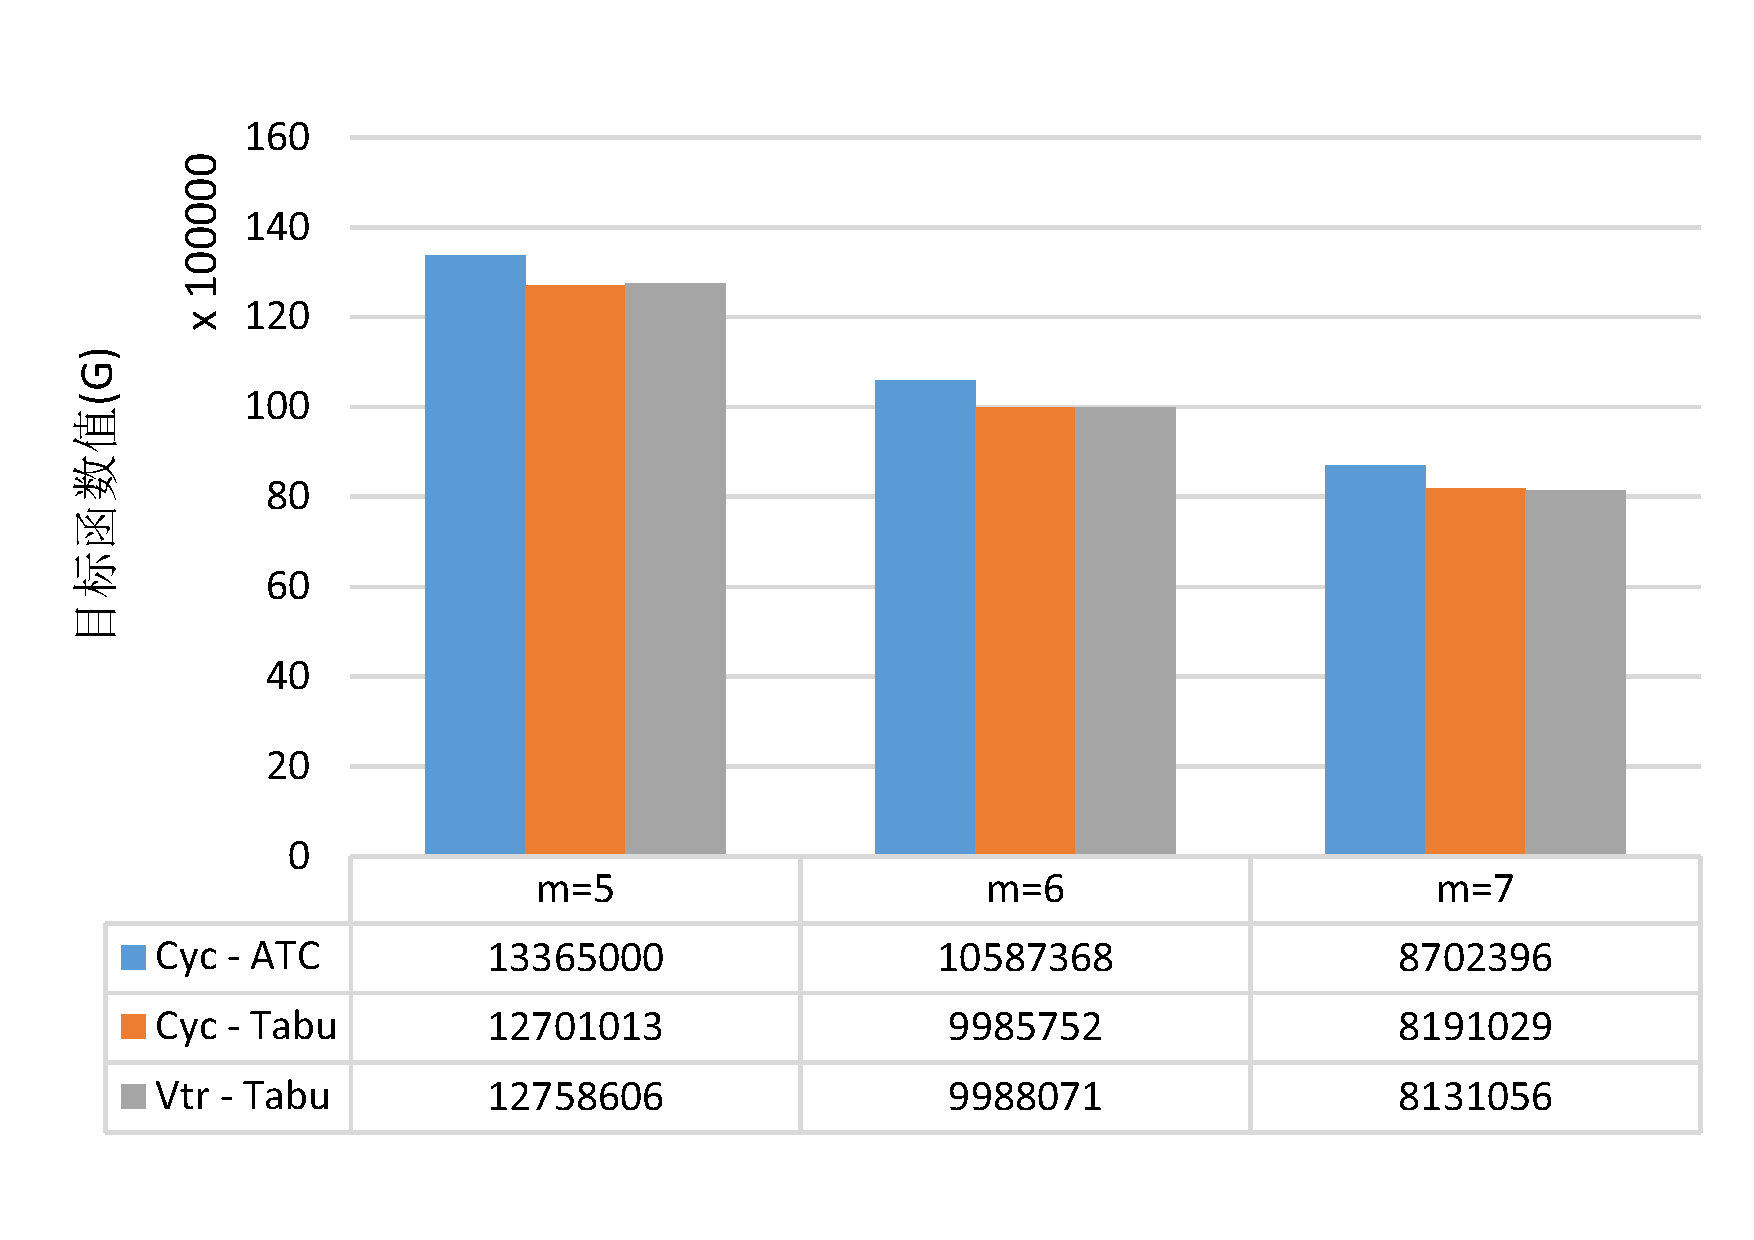
\includegraphics[height = 6cm, angle = -90]{basic_04_1000}}
\caption{\label{fig:result1}模型$1$的Cyc -- ATC、Cyc -- Tabu、Vtr -- Tabu 算法求解目标函数值比较$(\lambda_1 = 0.4)$}
\end{sidewaysfigure}

\begin{sidewaysfigure}
\centering
\subfloat[$n = 20$]{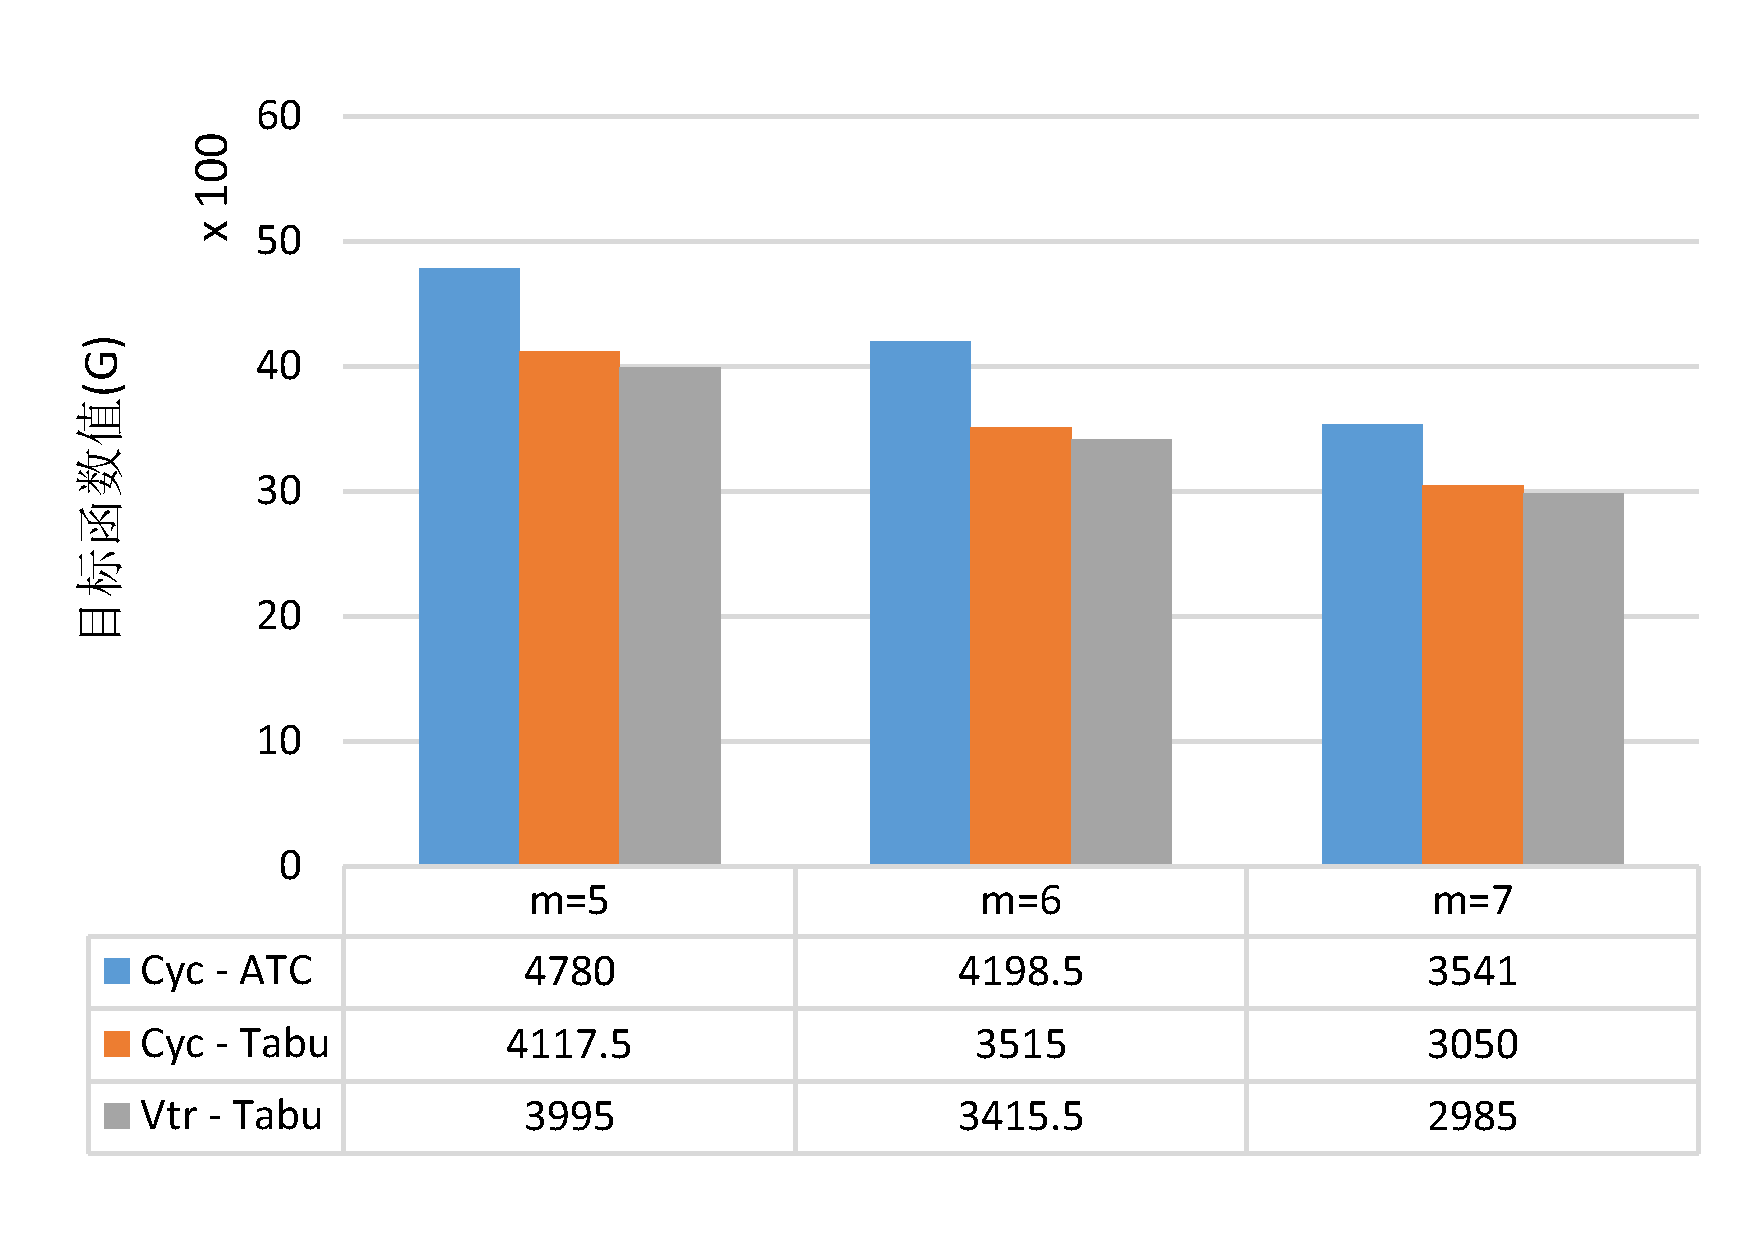
\includegraphics[height = 6cm, angle = -90]{basic_05_20}}
\subfloat[$n = 30$]{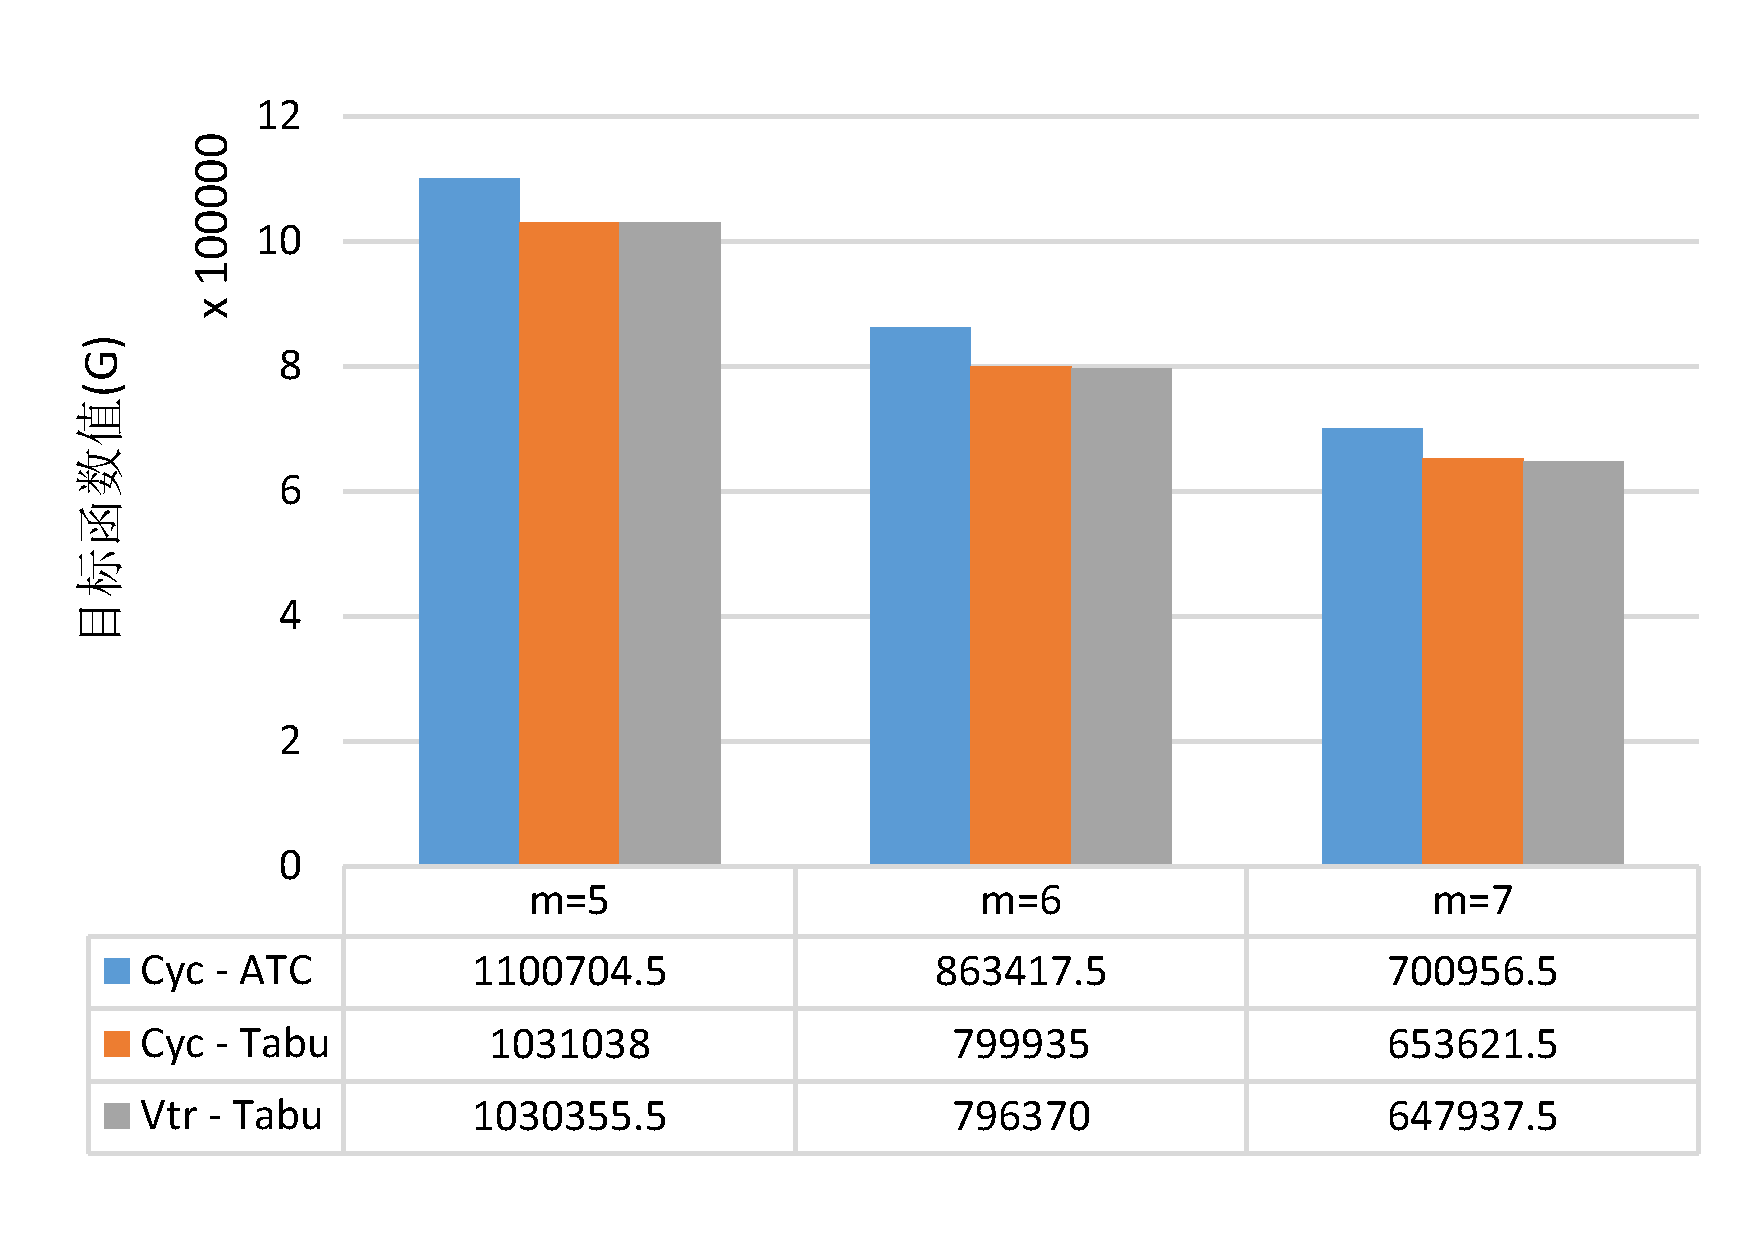
\includegraphics[height = 6cm, angle = -90]{basic_05_300}}
\subfloat[$n = 50$]{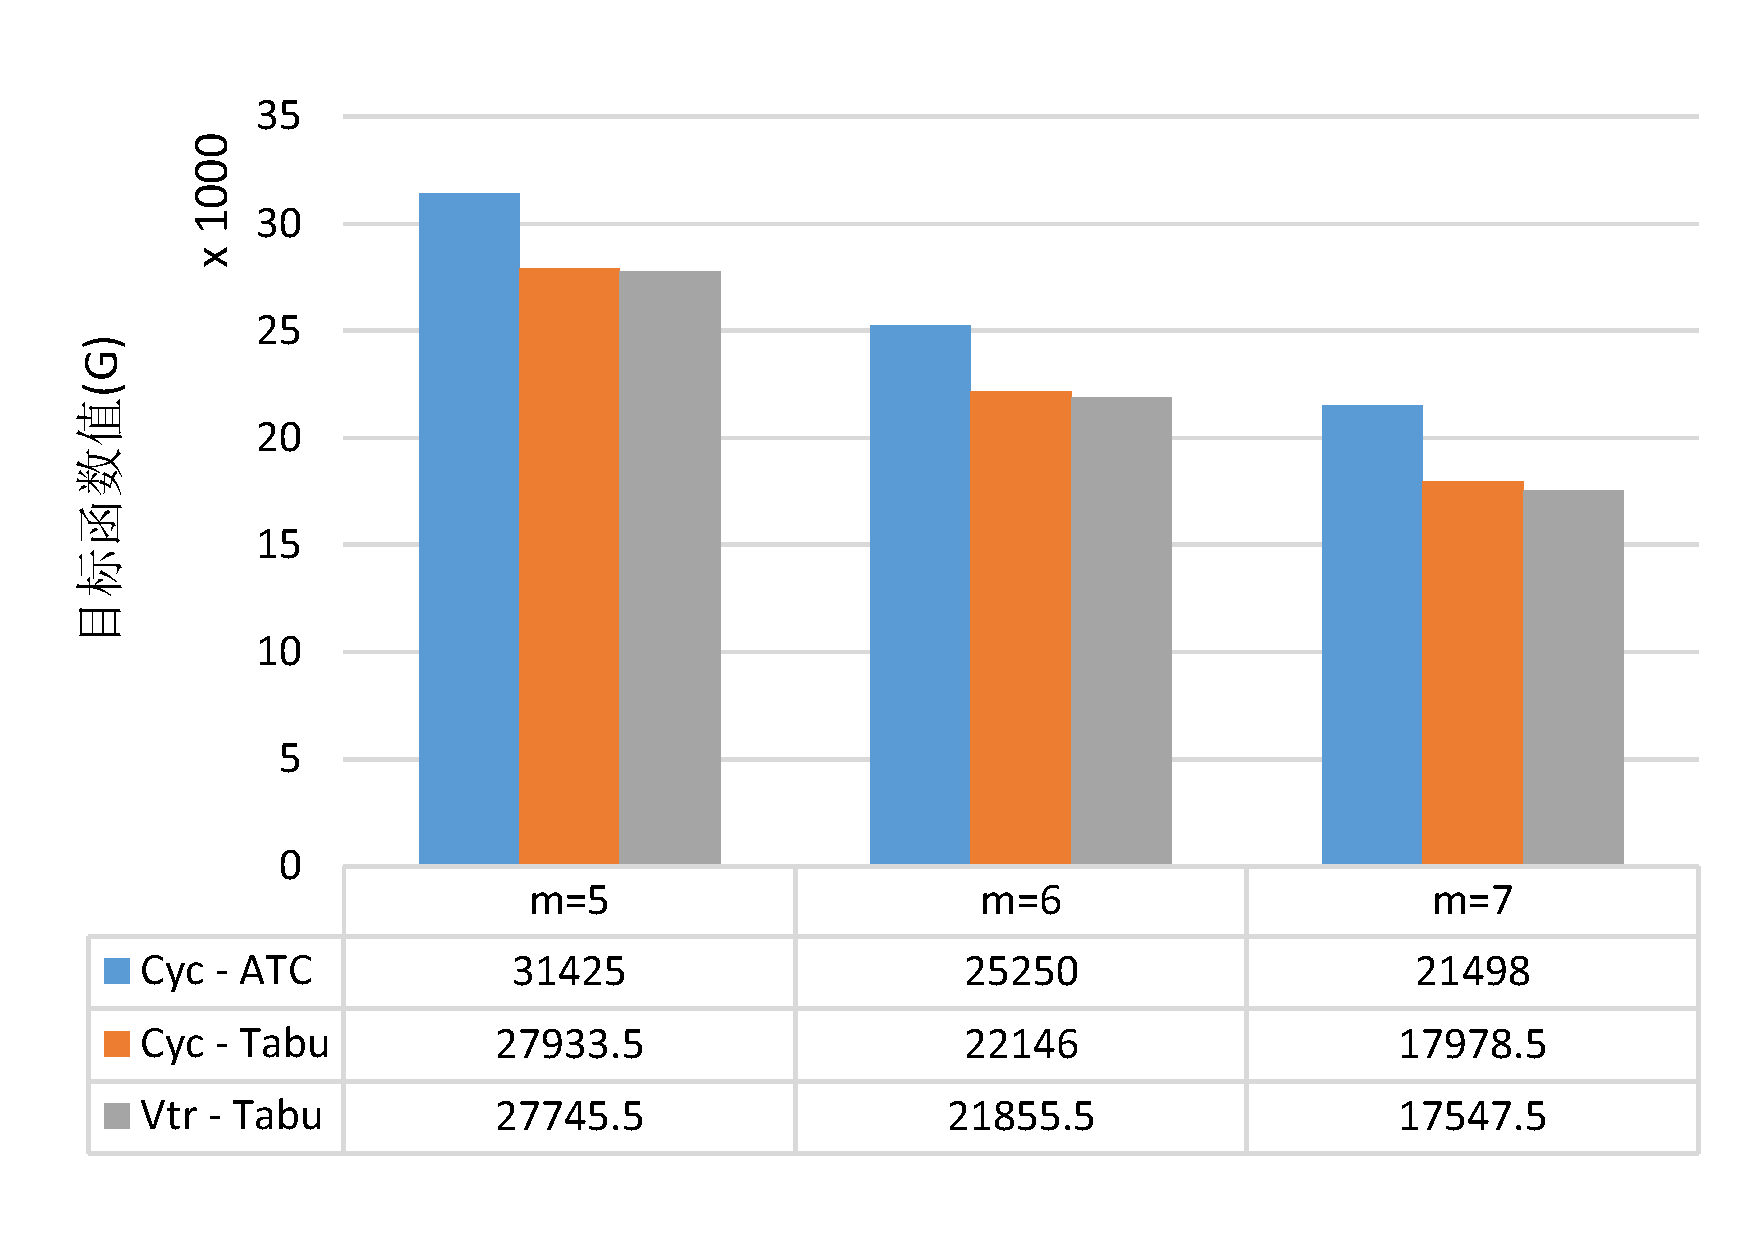
\includegraphics[height = 6cm, angle = -90]{basic_05_50}}
\subfloat[$n = 70$]{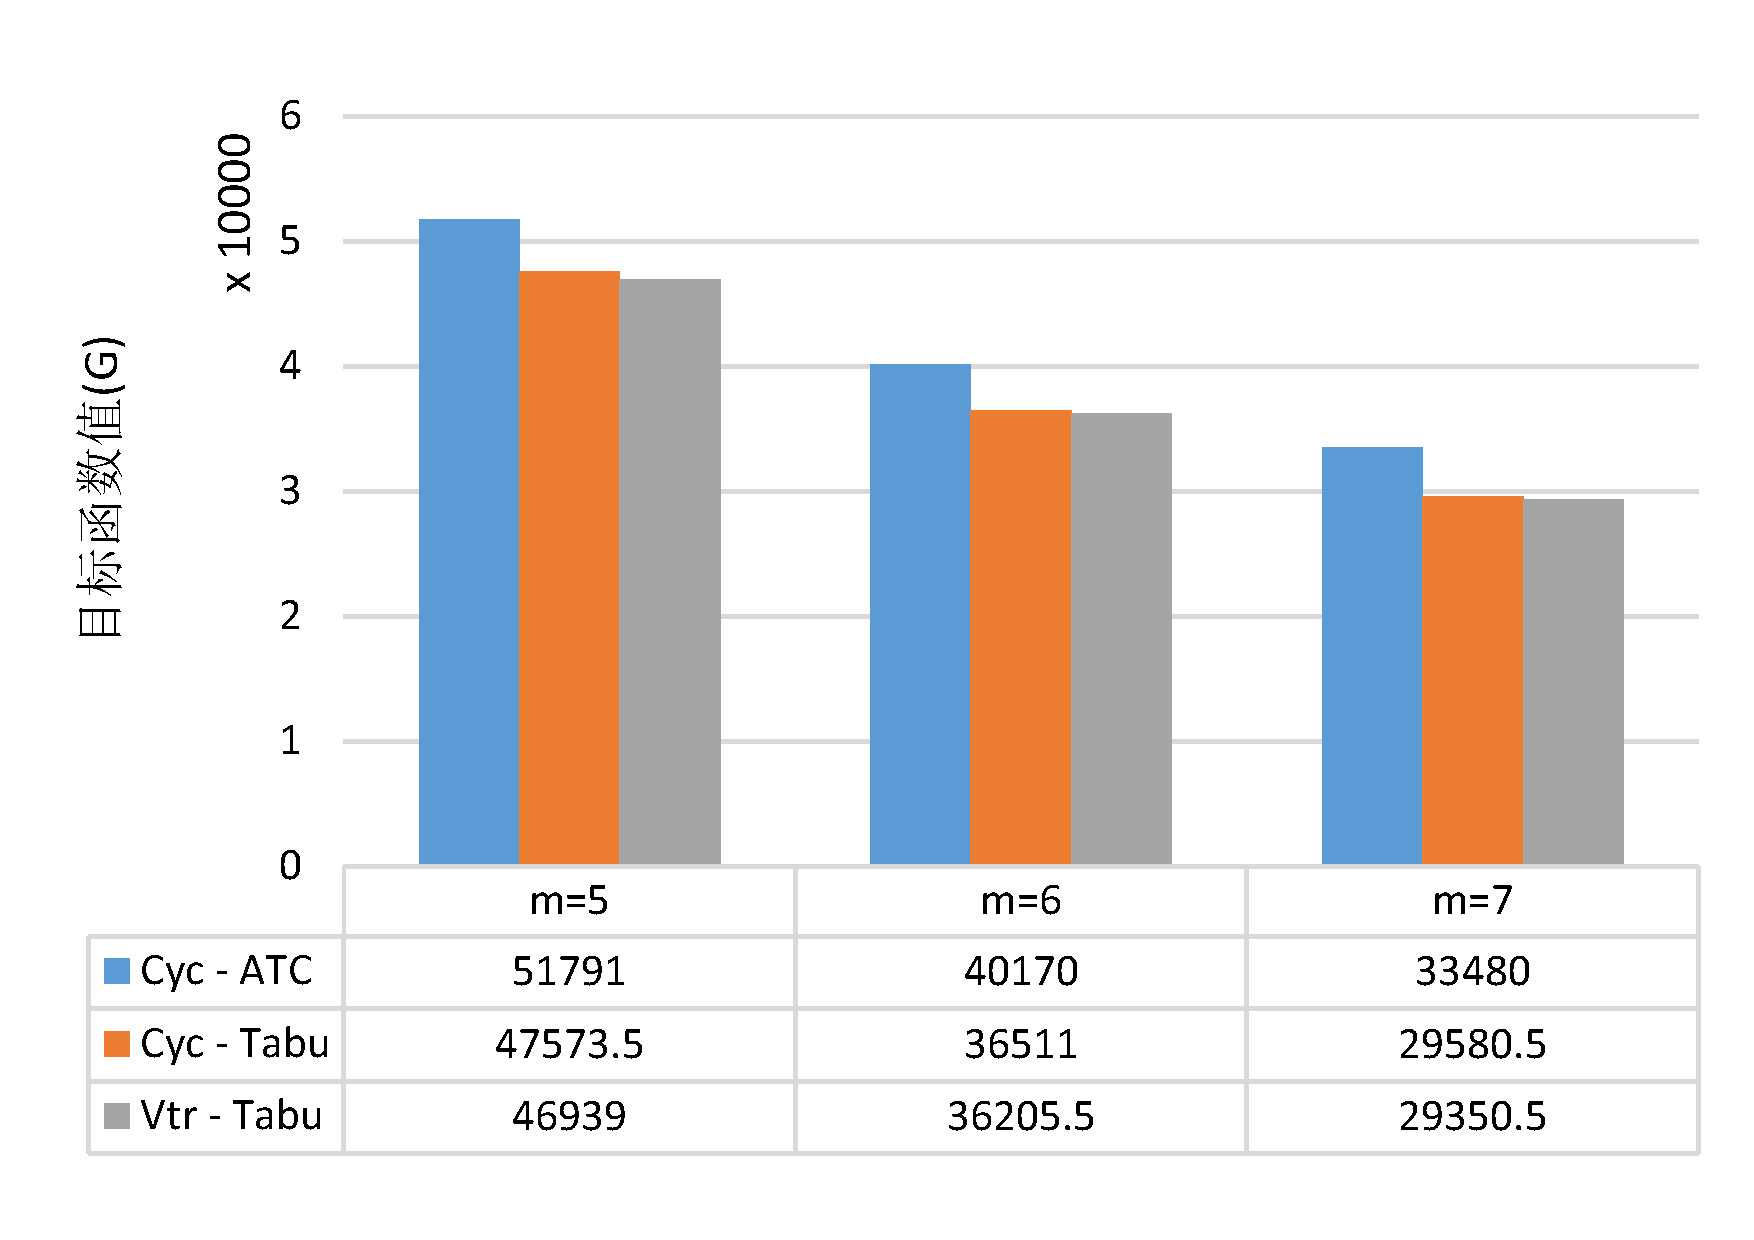
\includegraphics[height = 6cm, angle = -90]{basic_05_70}}\\
\subfloat[$n = 100$]{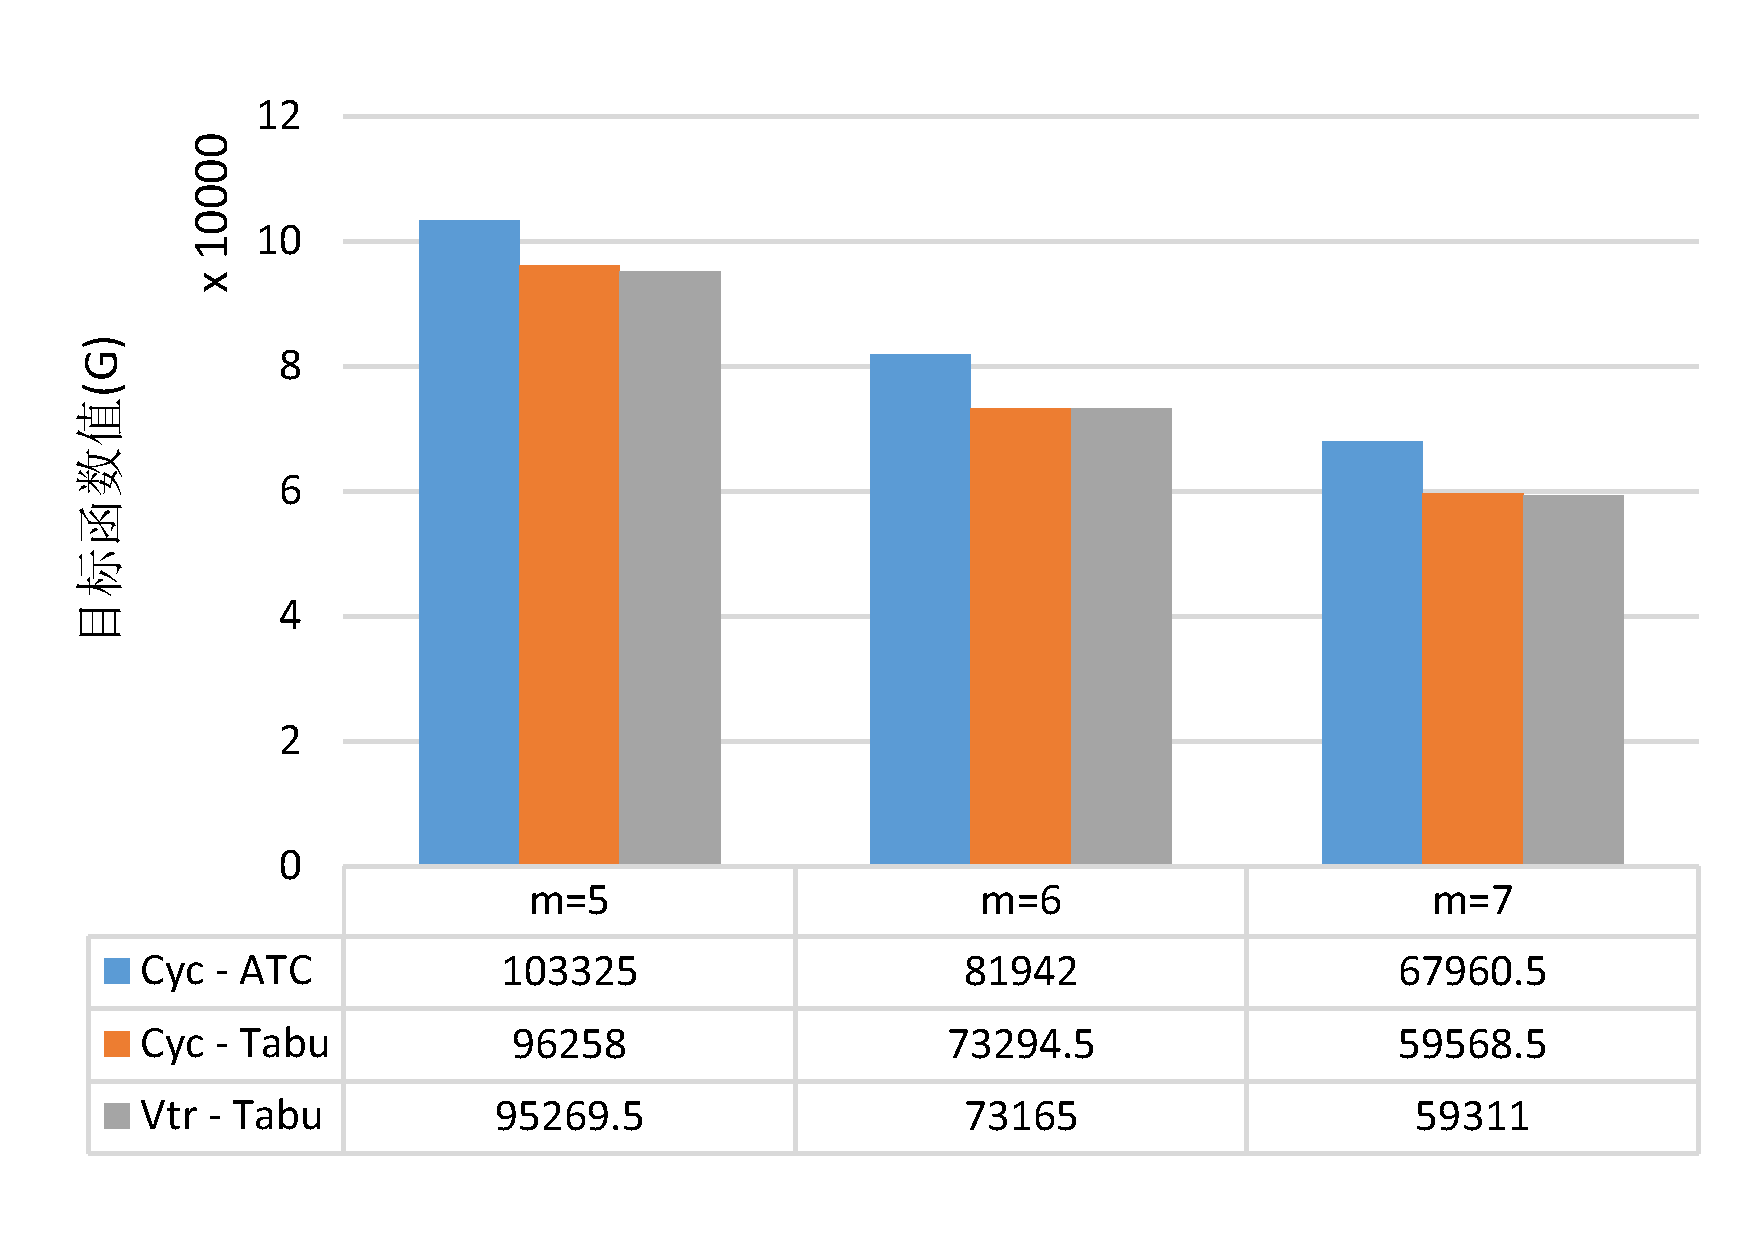
\includegraphics[height = 6cm, angle = -90]{basic_05_100}}
\subfloat[$n = 150$]{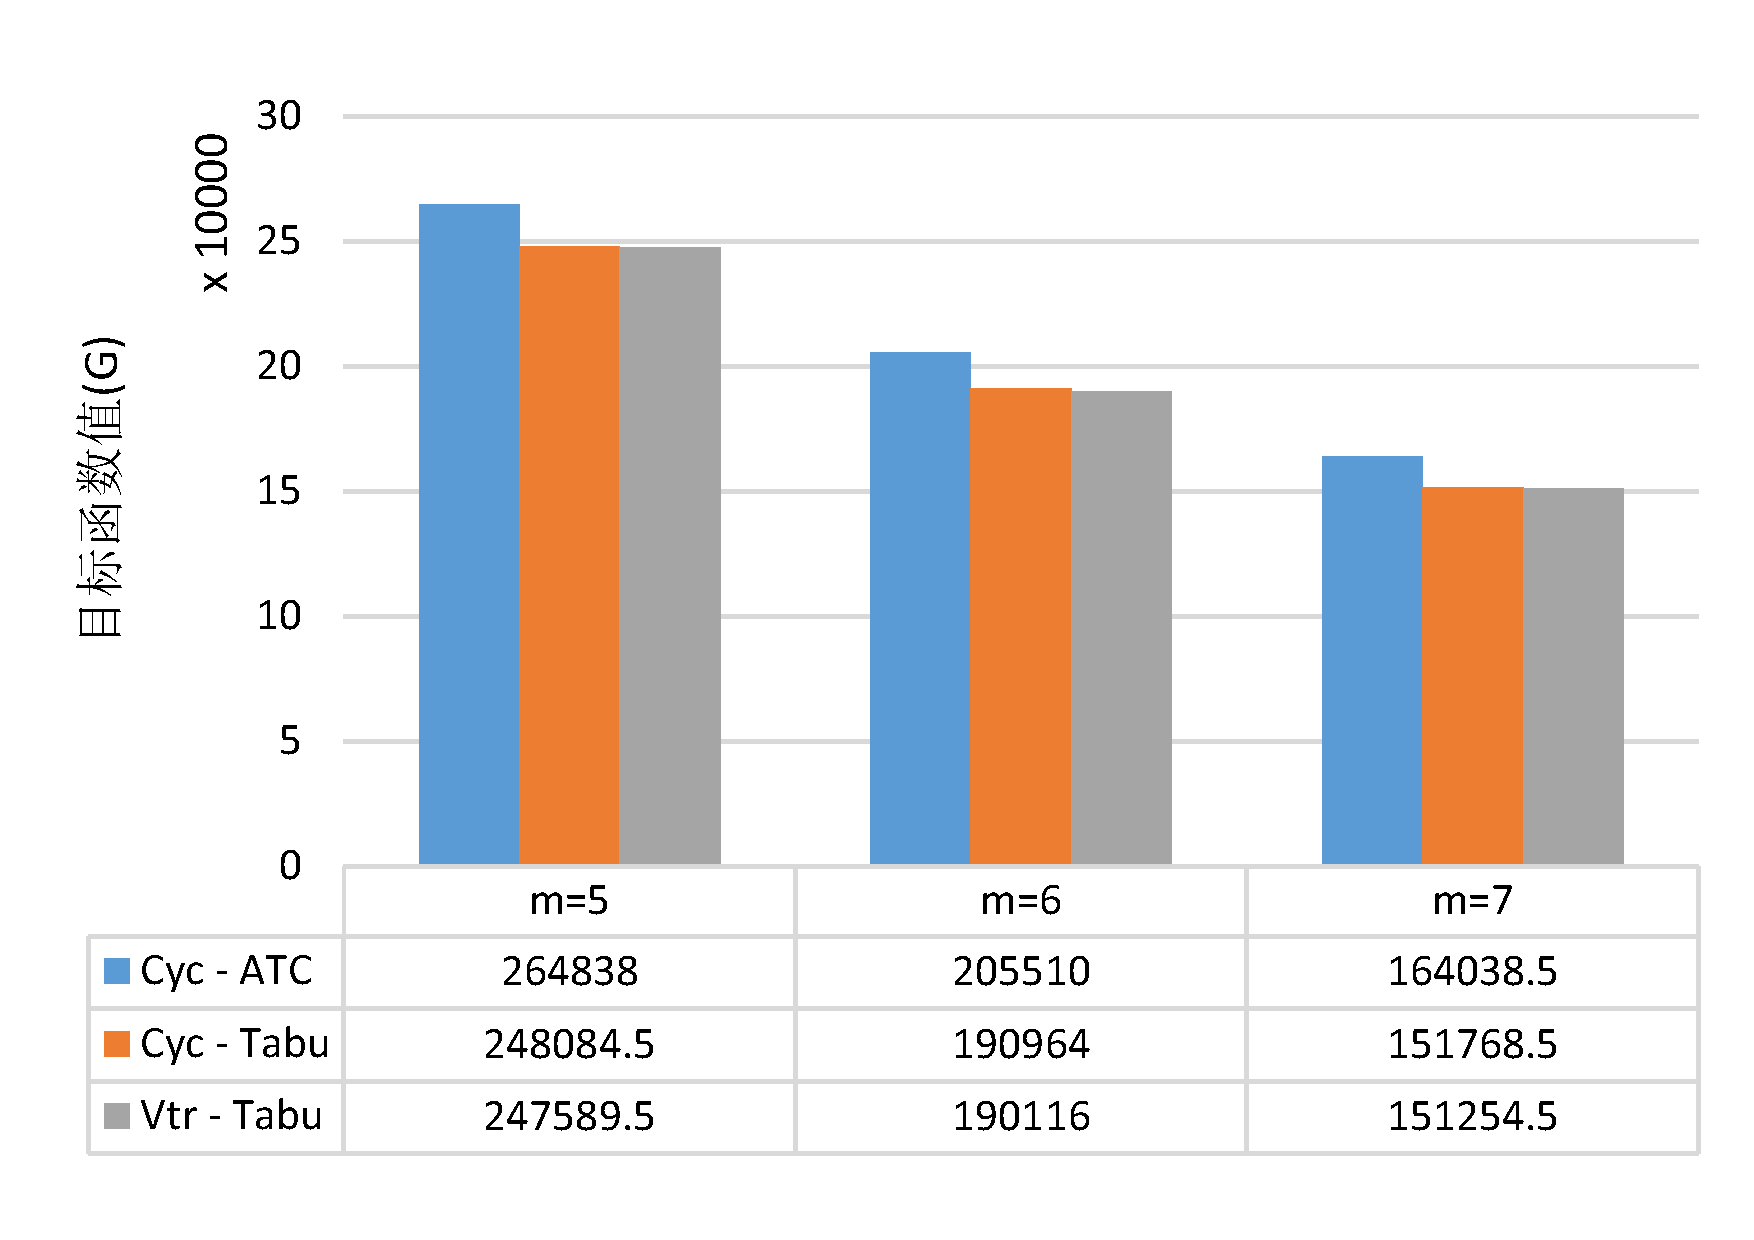
\includegraphics[height = 6cm, angle = -90]{basic_05_150}}
\subfloat[$n = 200$]{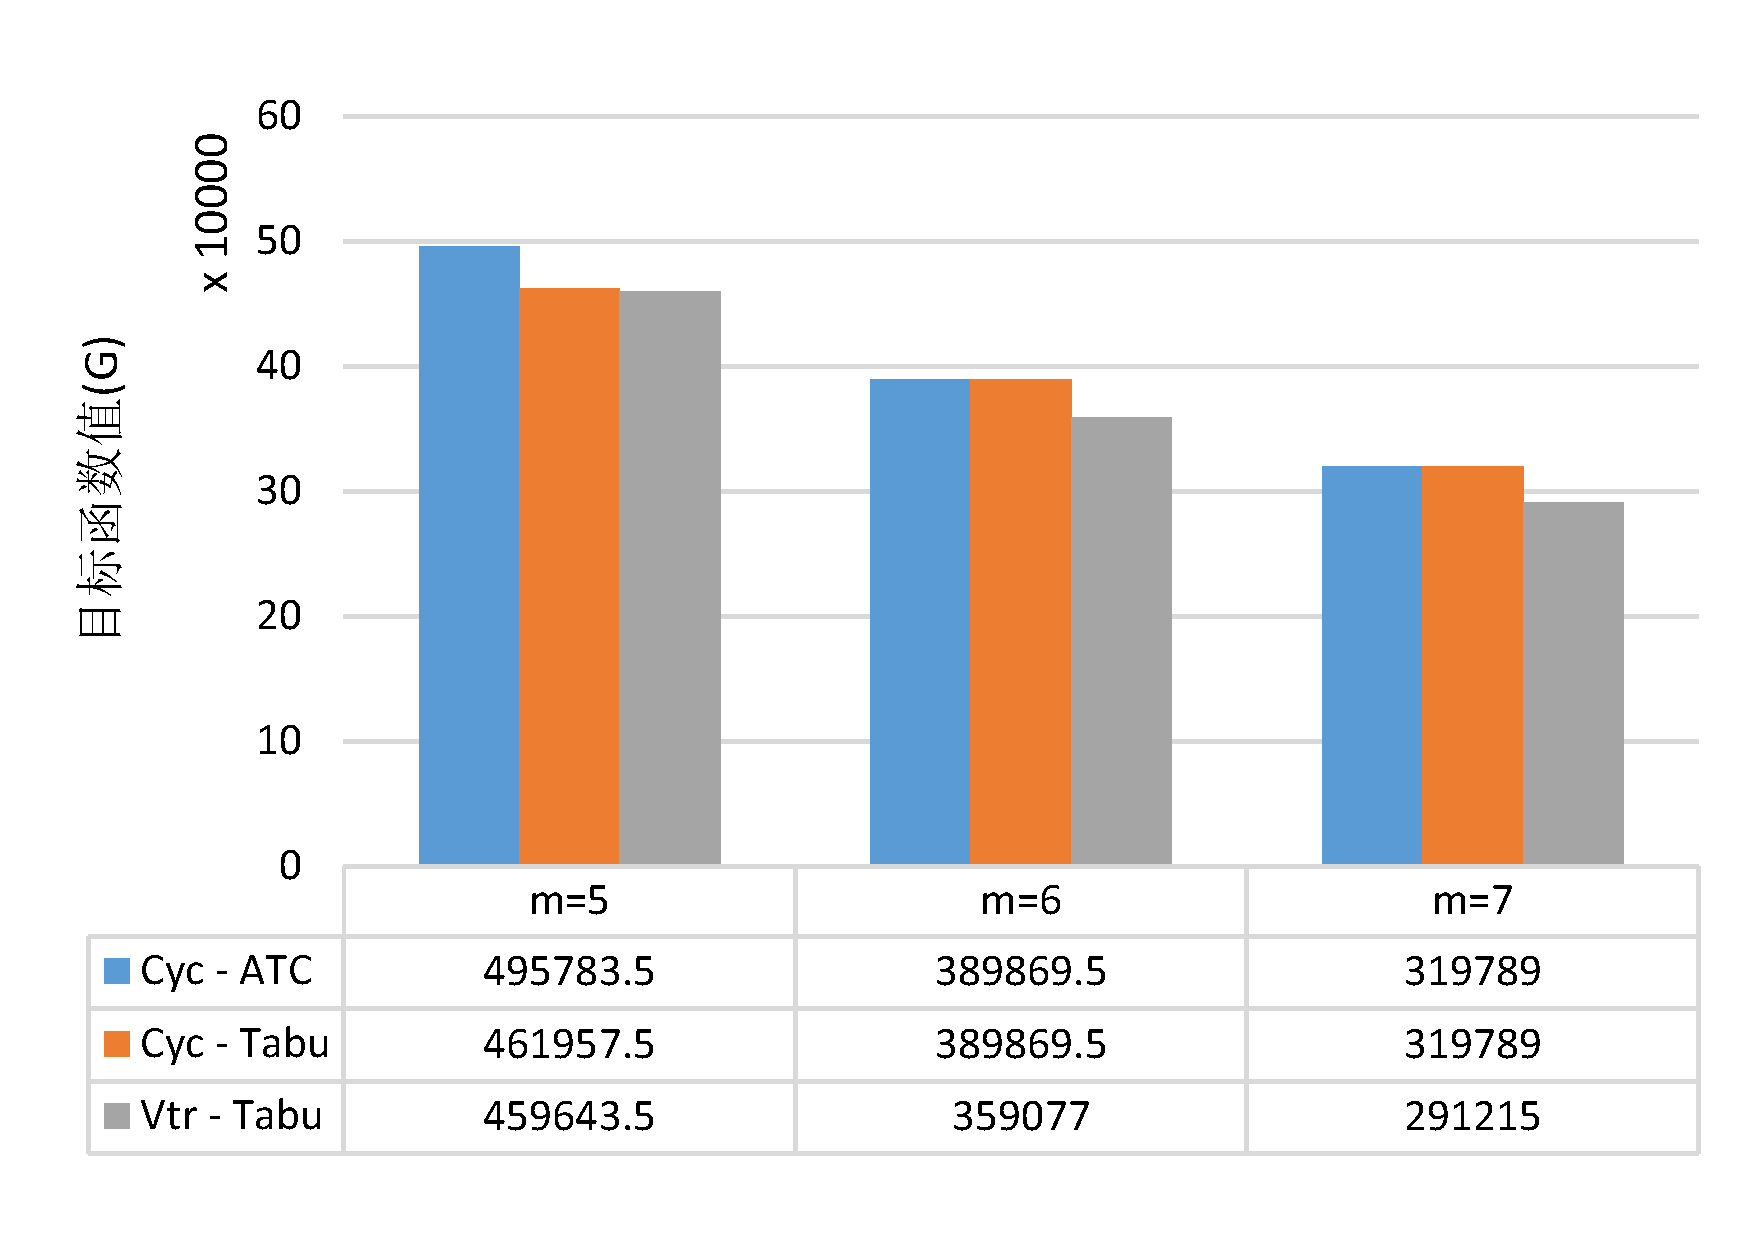
\includegraphics[height = 6cm, angle = -90]{basic_05_200}}
\subfloat[$n = 300$]{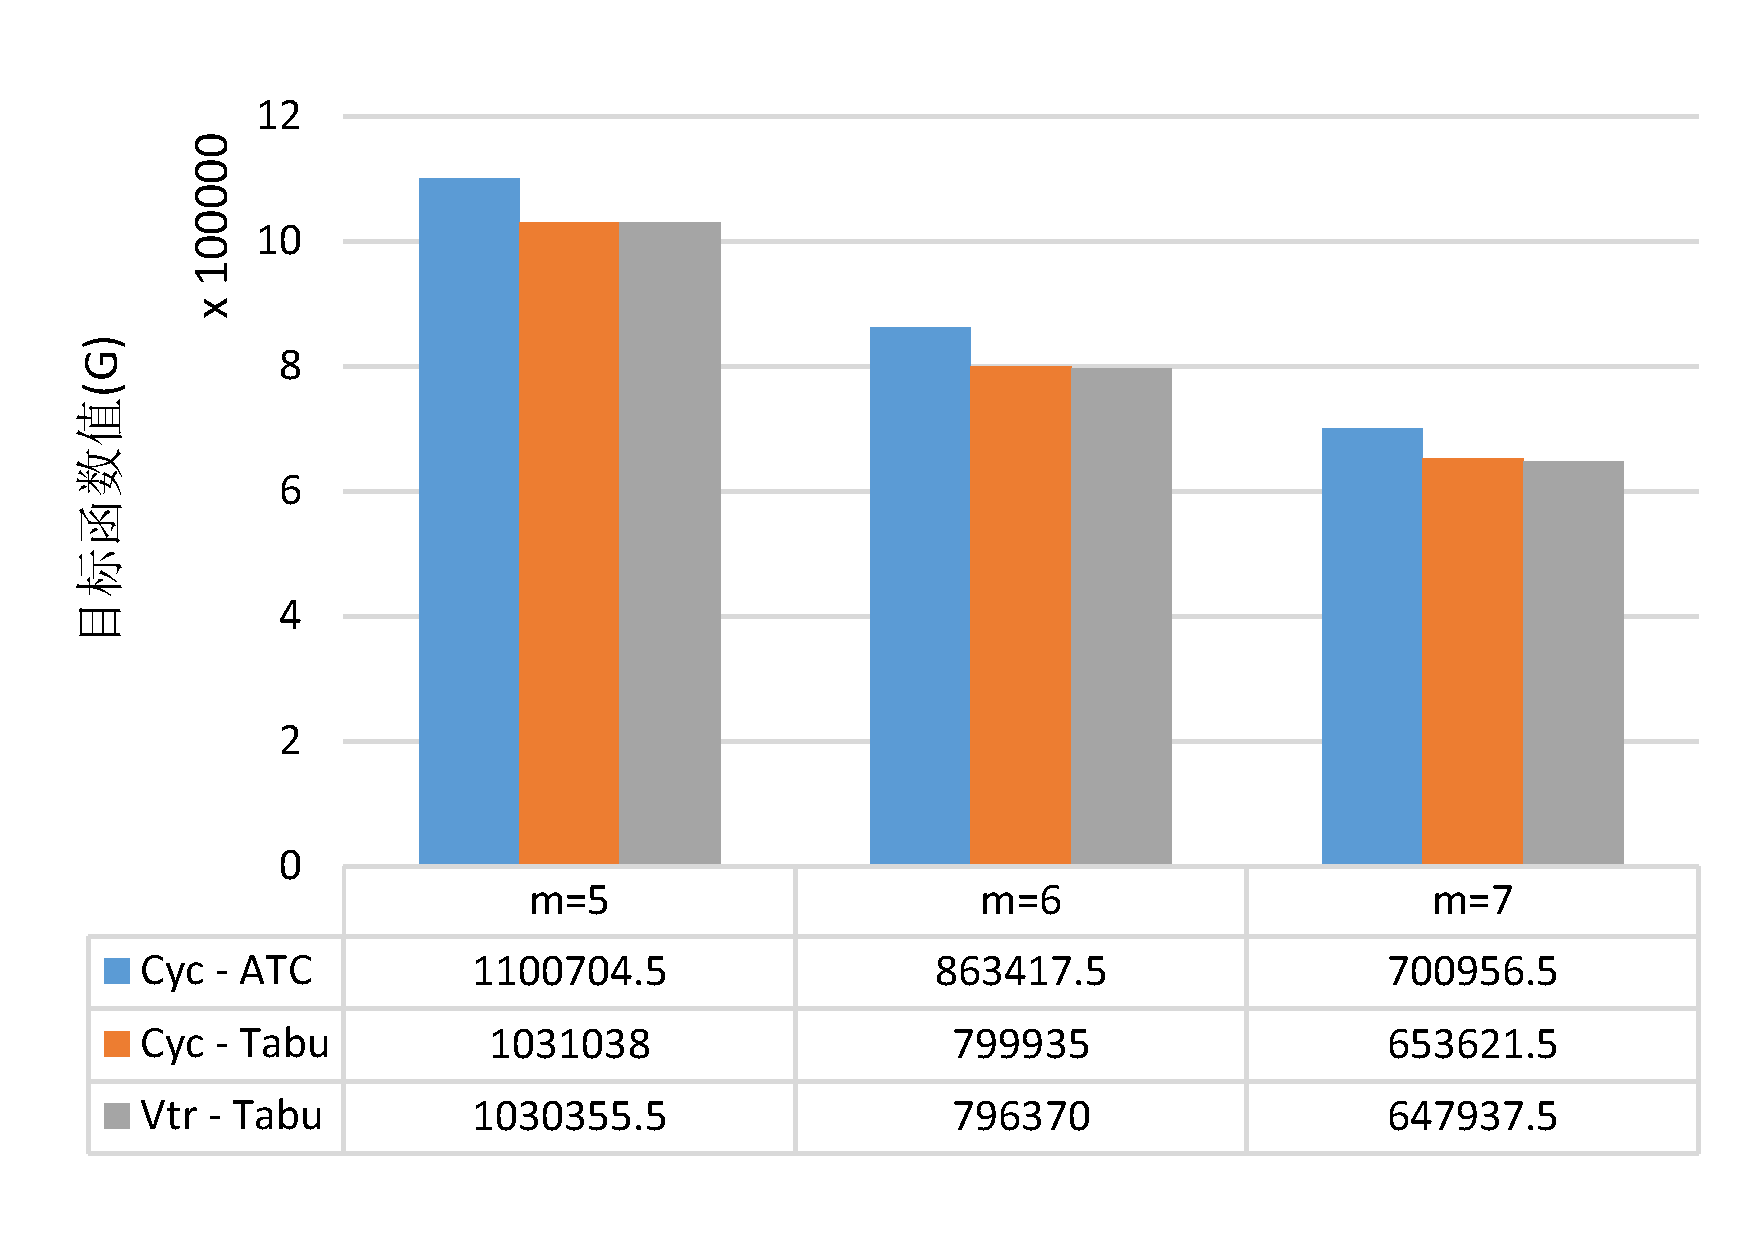
\includegraphics[height = 6cm, angle = -90]{basic_05_300}}\\
\subfloat[$n = 500$]{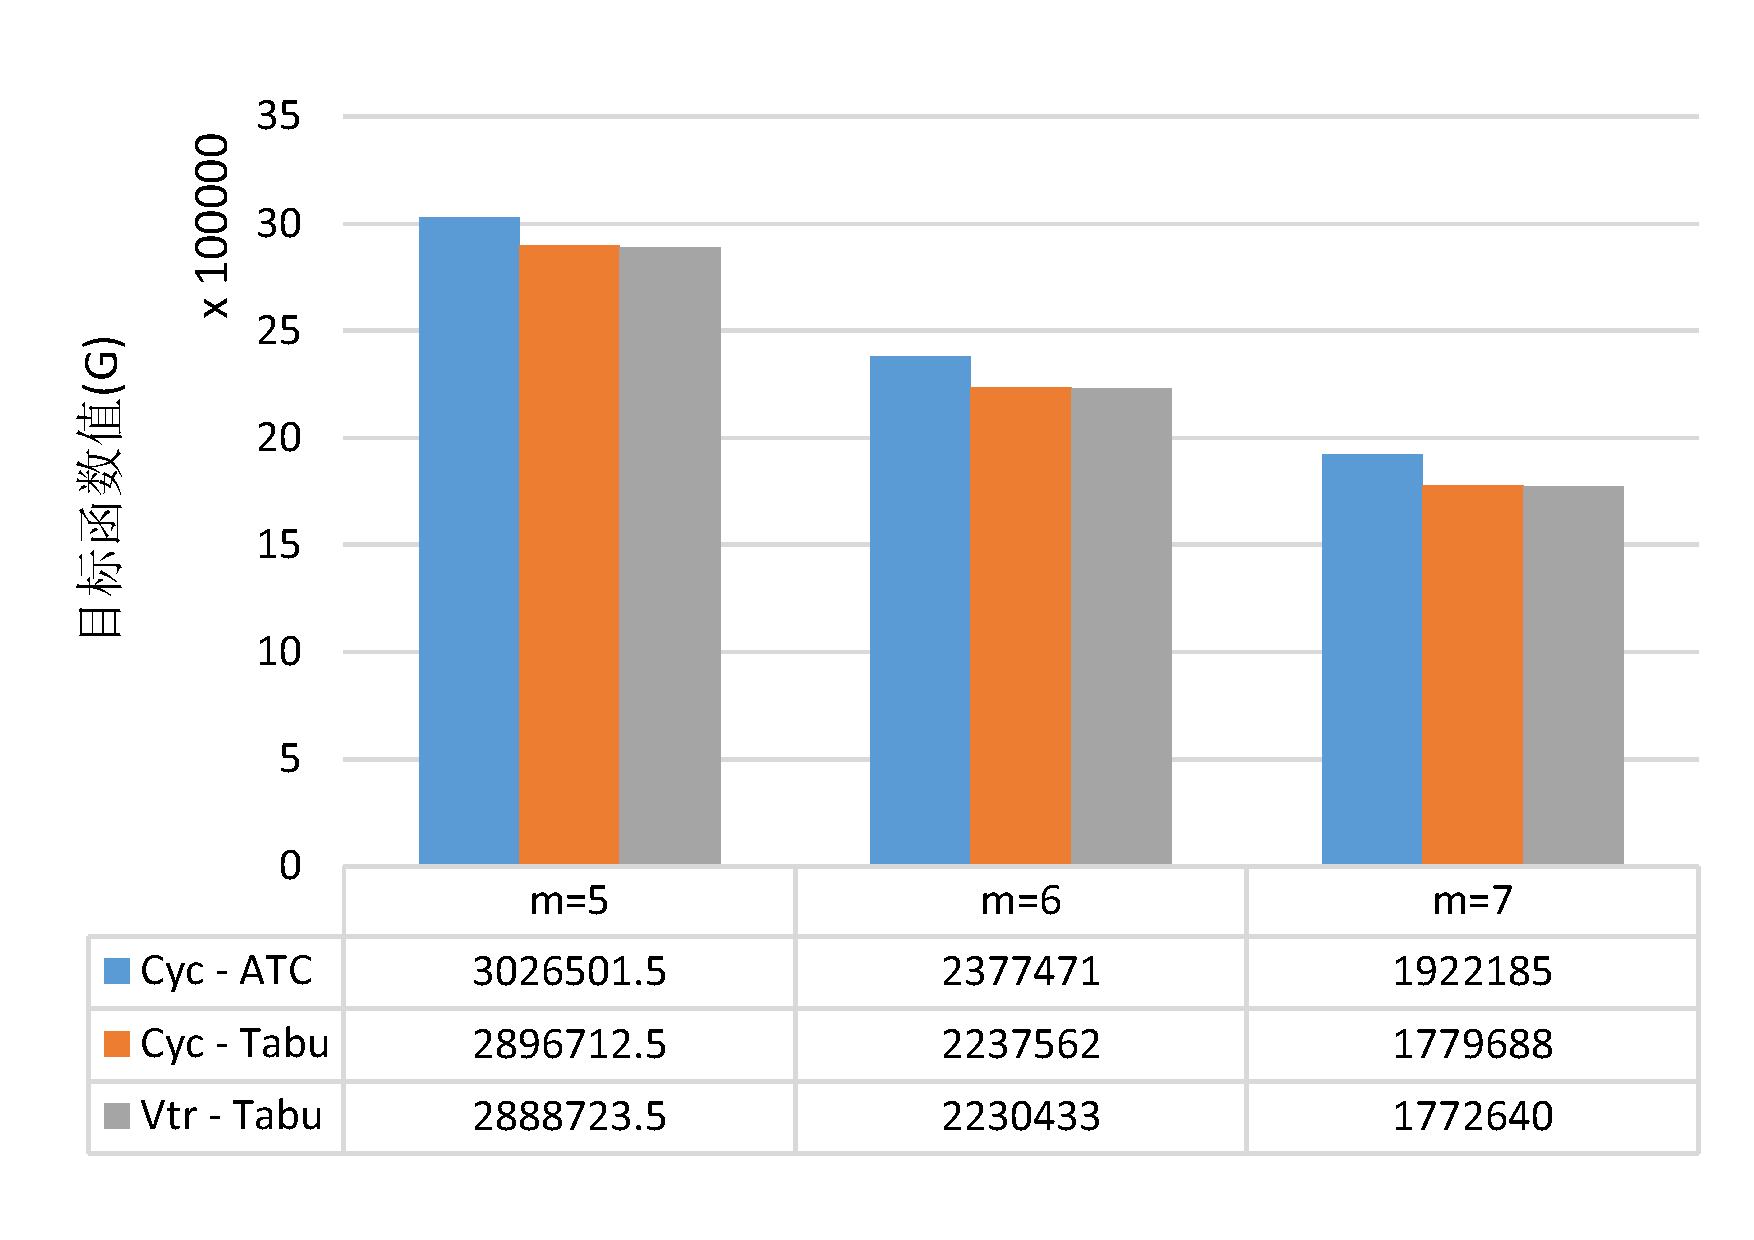
\includegraphics[height = 6cm, angle = -90]{basic_05_500}}
\subfloat[$n = 750$]{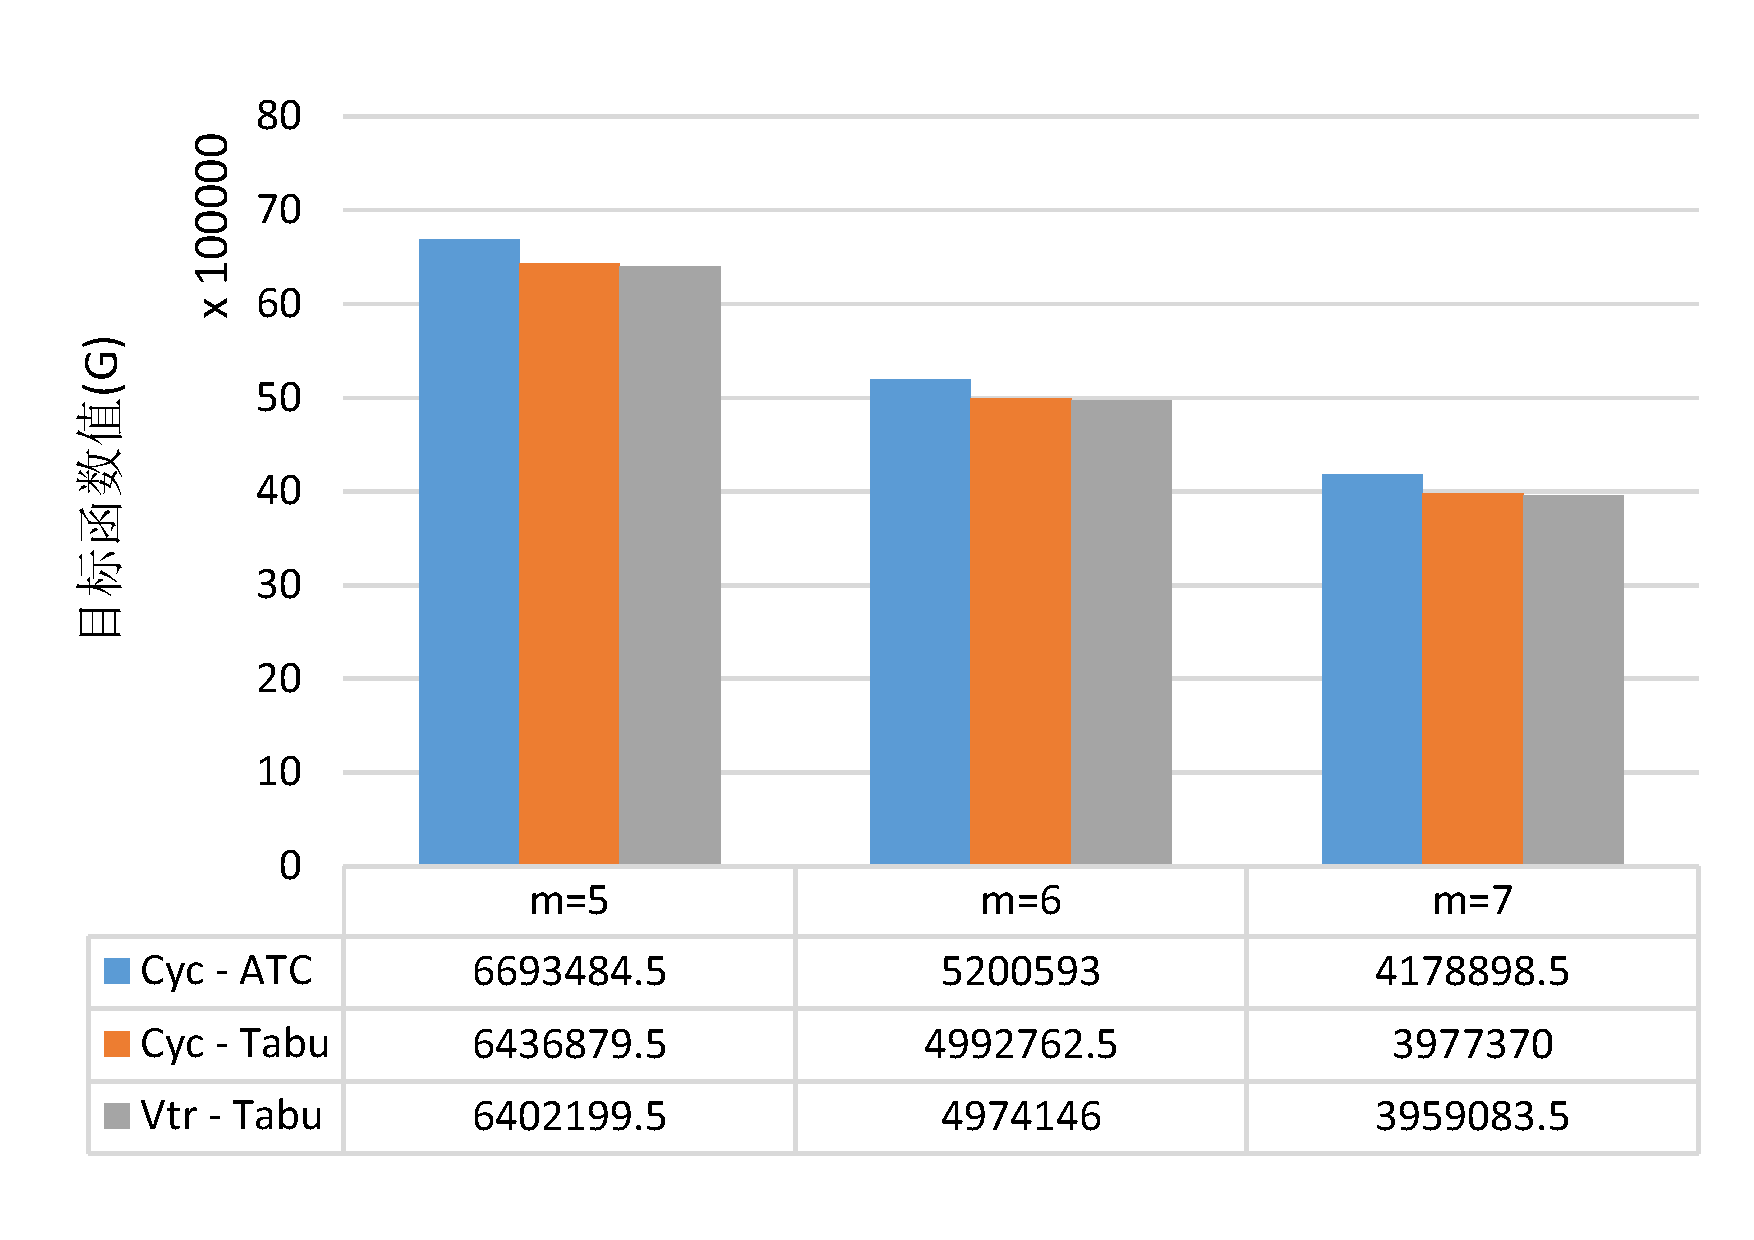
\includegraphics[height = 6cm, angle = -90]{basic_05_750}}
\subfloat[$n = 1000$]{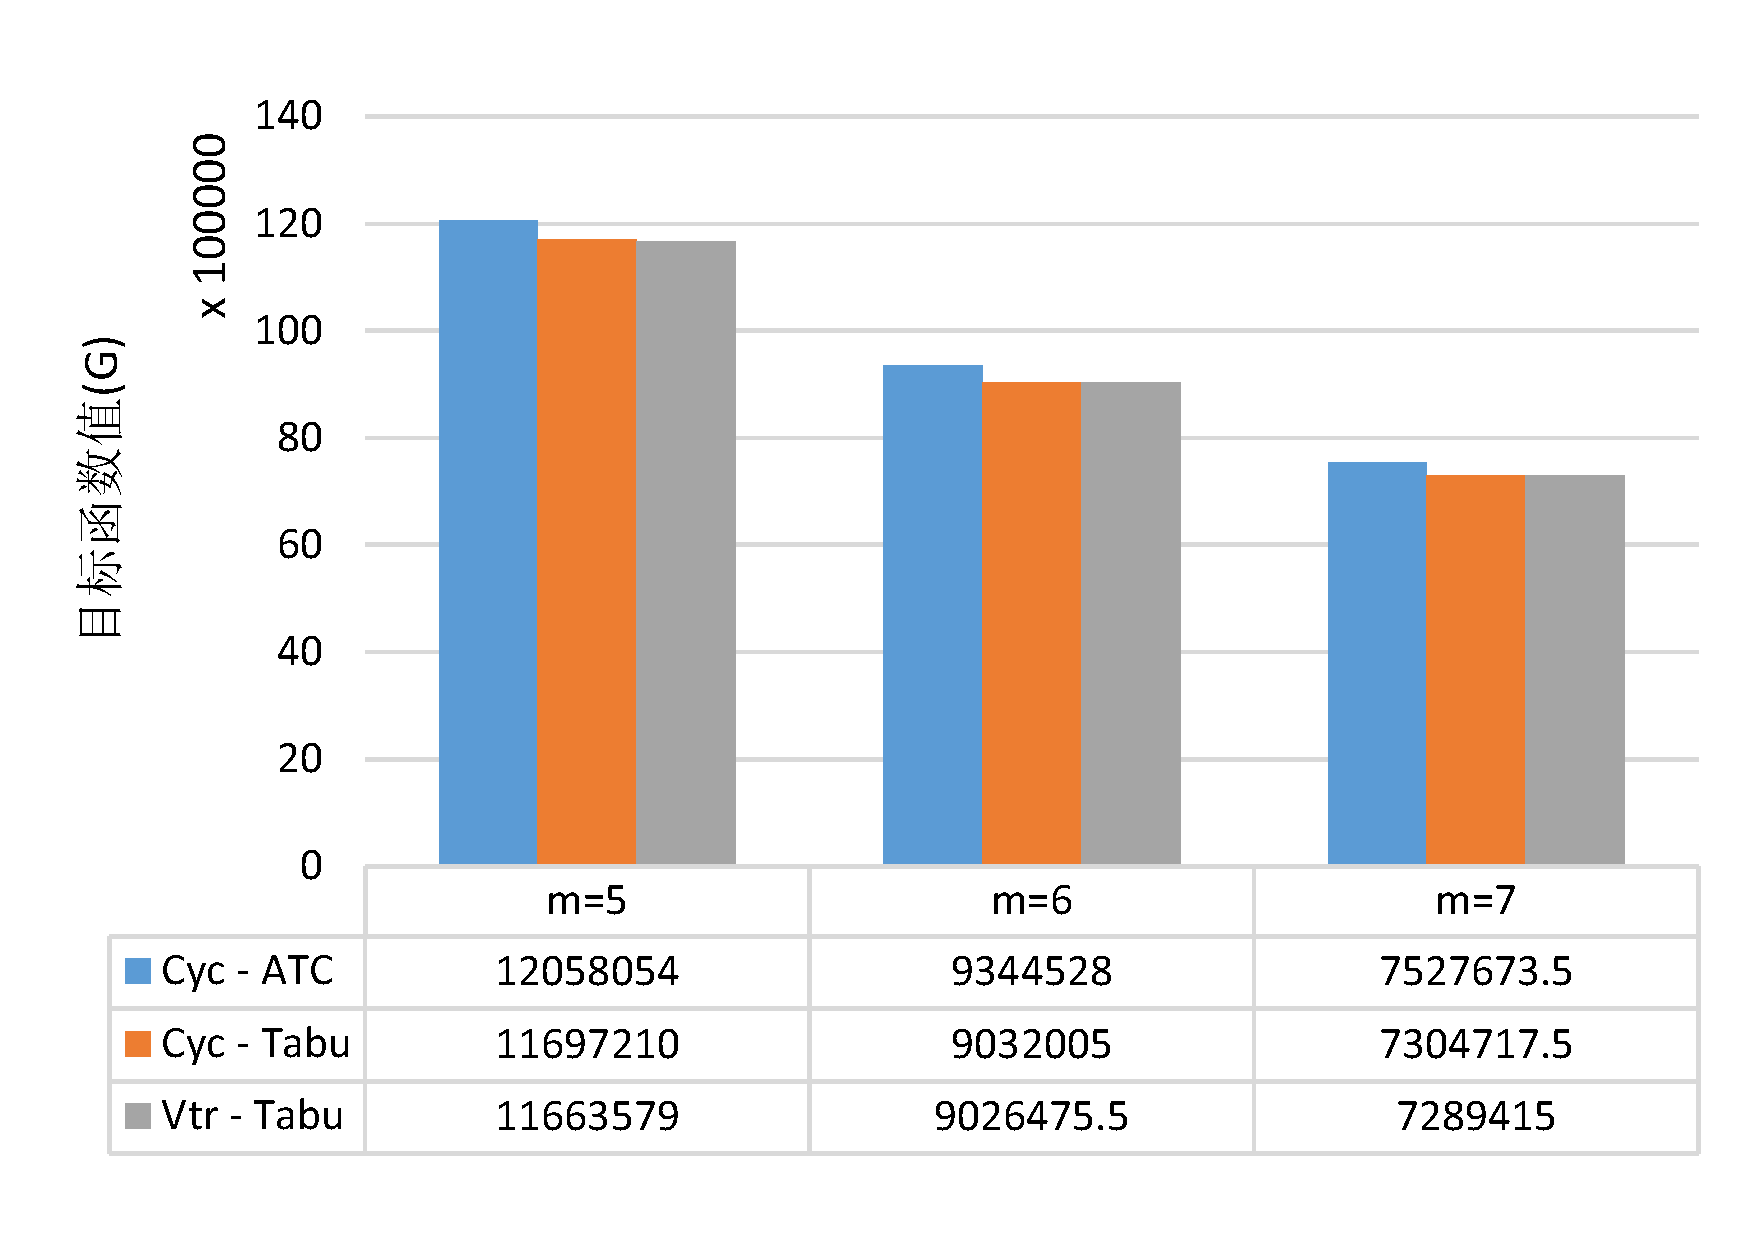
\includegraphics[height = 6cm, angle = -90]{basic_05_1000}}
\caption{\label{fig:result2}模型$1$的Cyc -- ATC、Cyc -- Tabu、Vtr -- Tabu 算法求解目标函数值比较$(\lambda_1 = 0.5)$}
\end{sidewaysfigure}

\begin{sidewaysfigure}
\centering
\subfloat[$n = 20$]{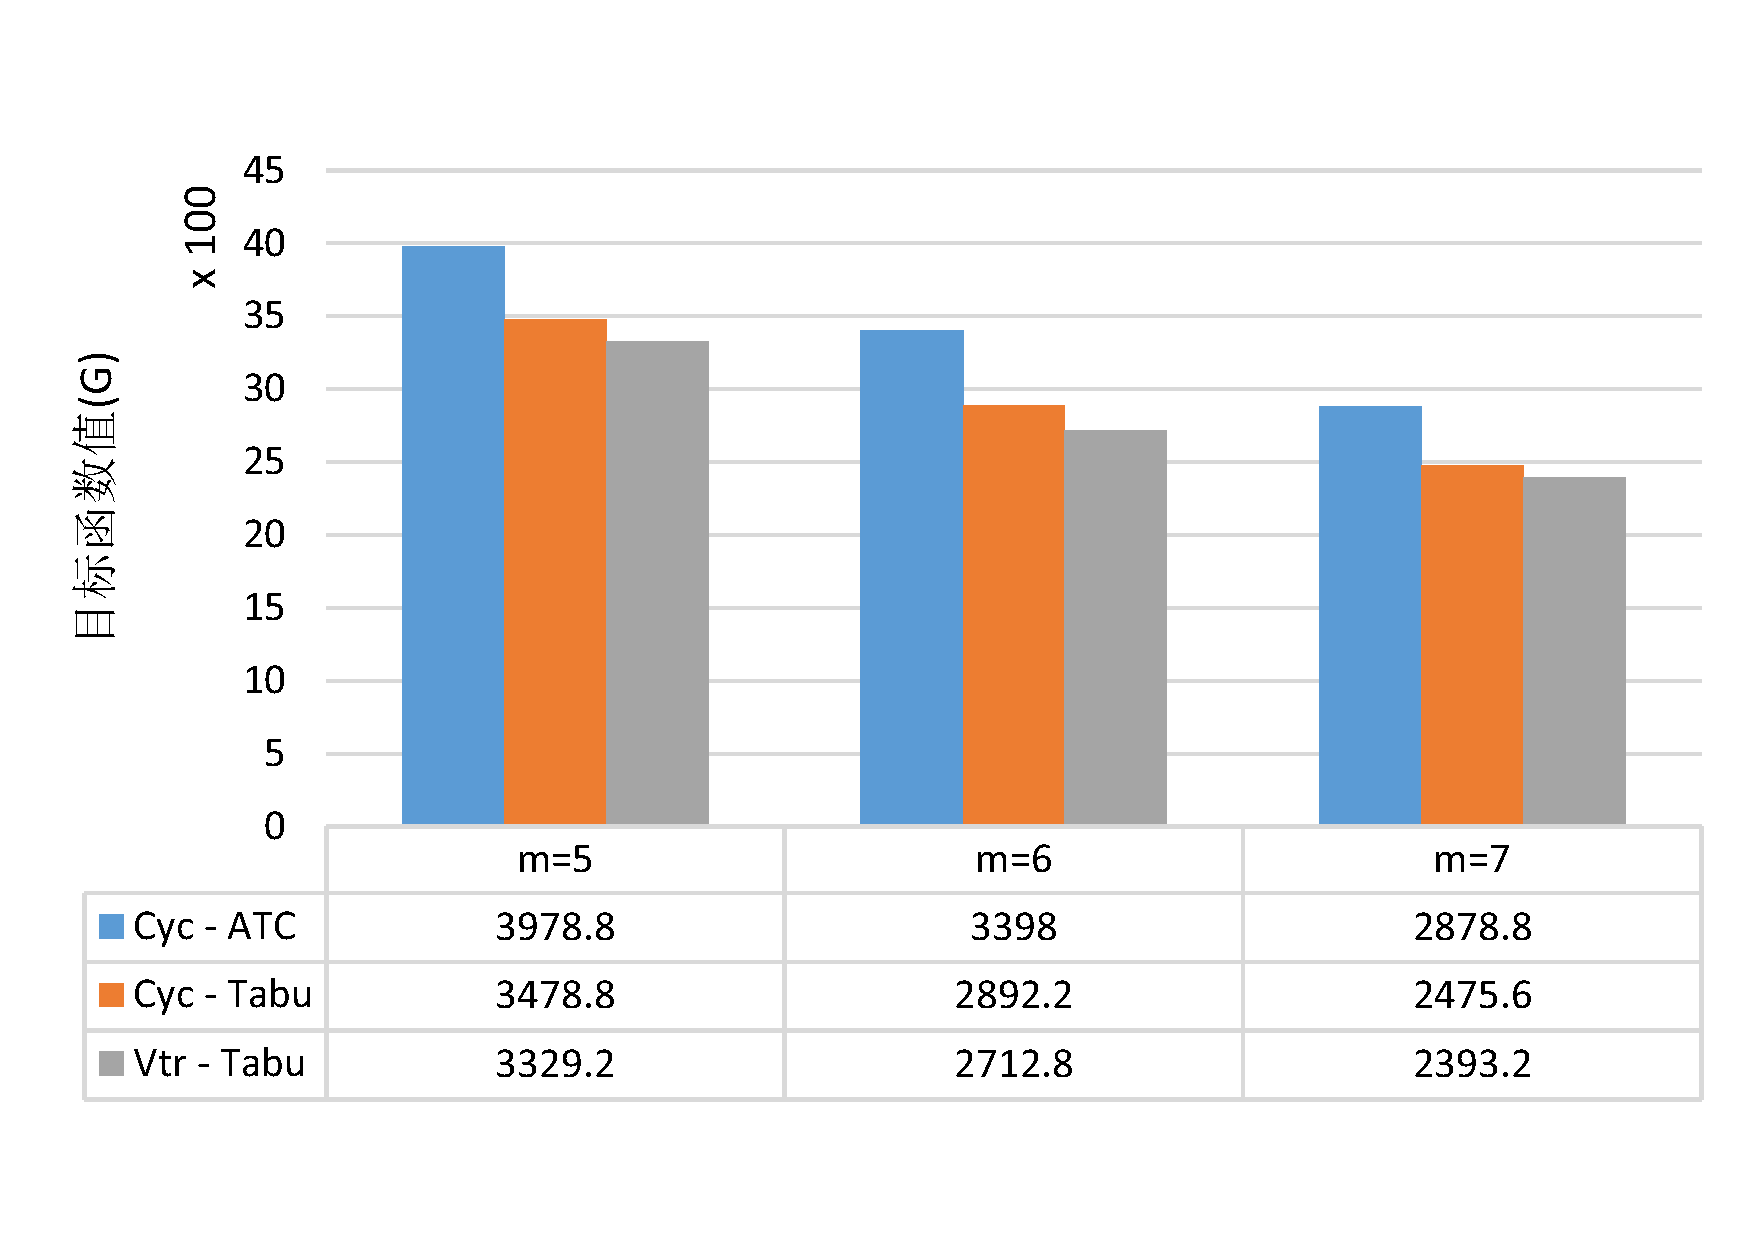
\includegraphics[height = 6cm, angle = -90]{basic_06_20}}
\subfloat[$n = 30$]{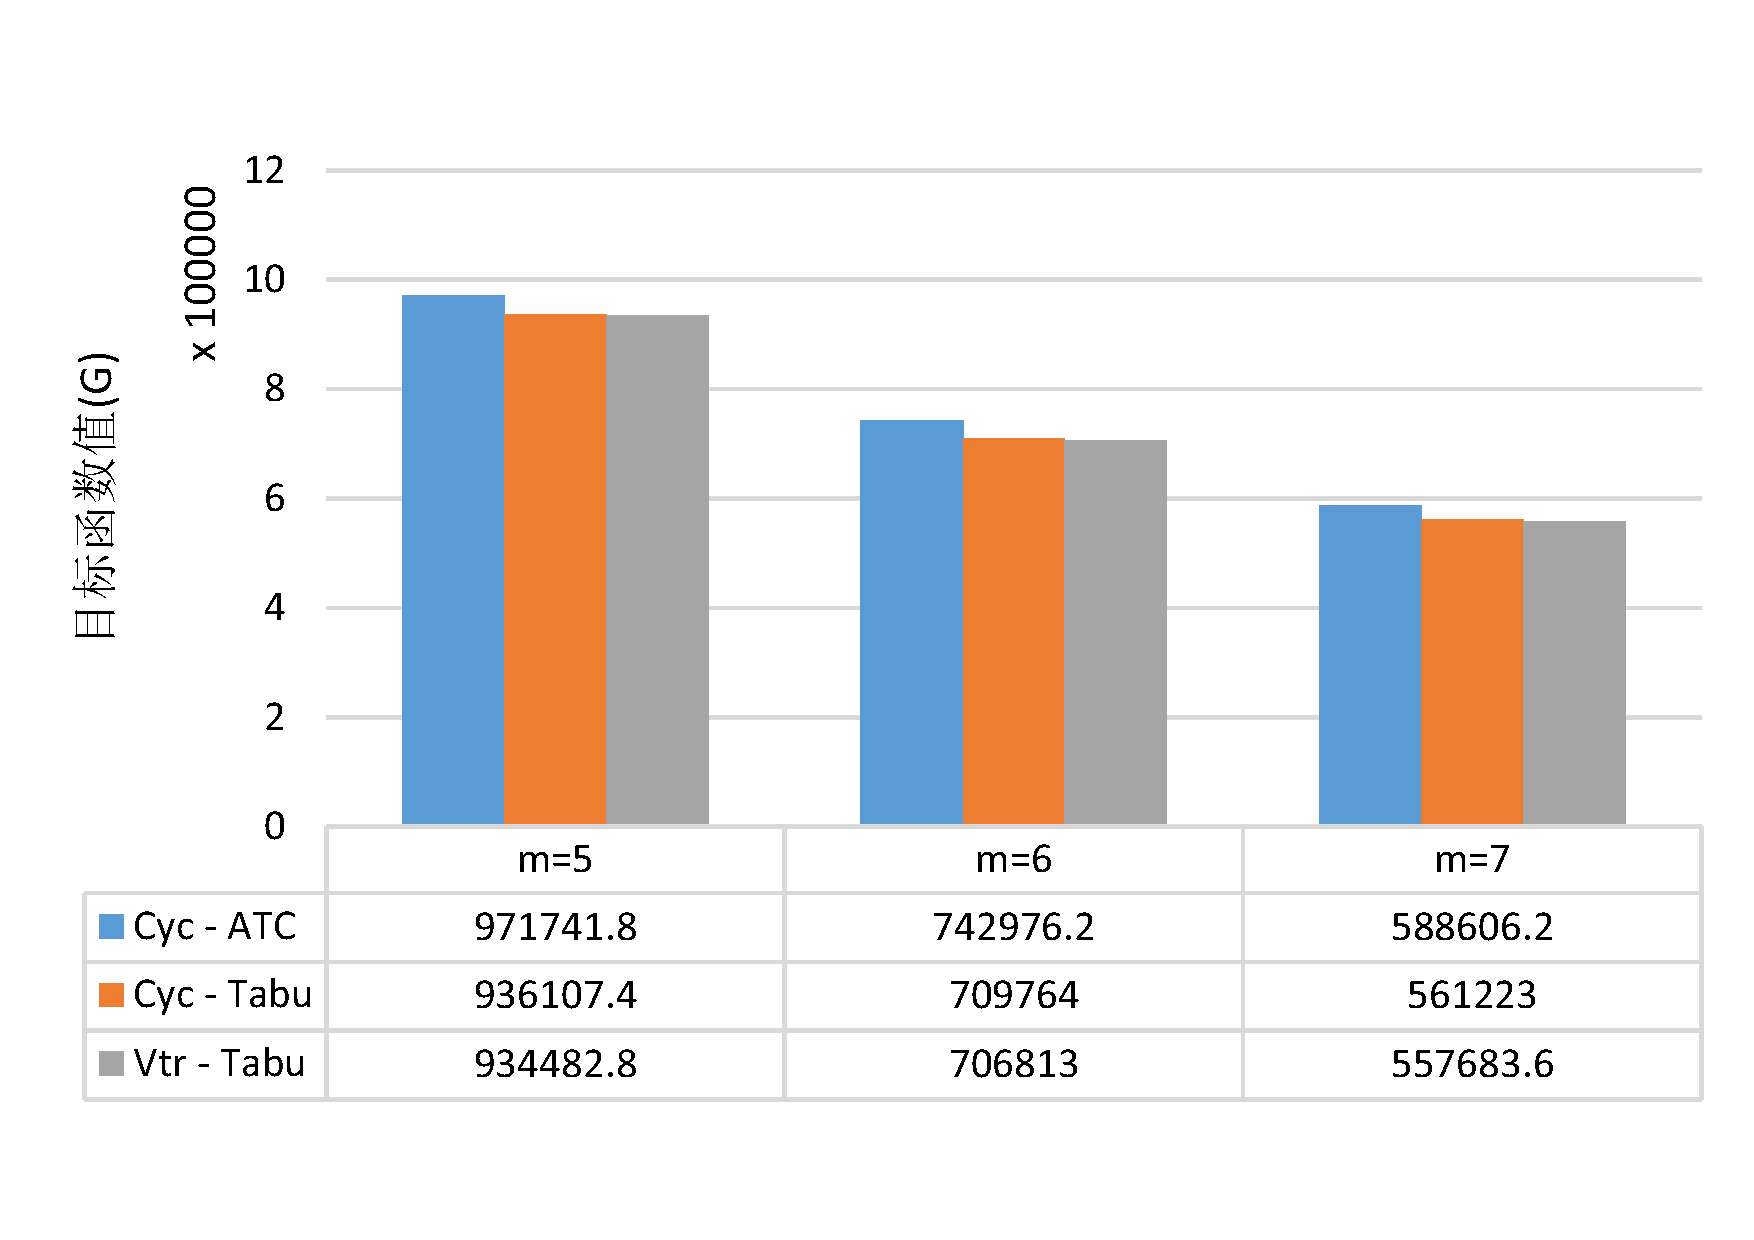
\includegraphics[height = 6cm, angle = -90]{basic_06_300}}
\subfloat[$n = 50$]{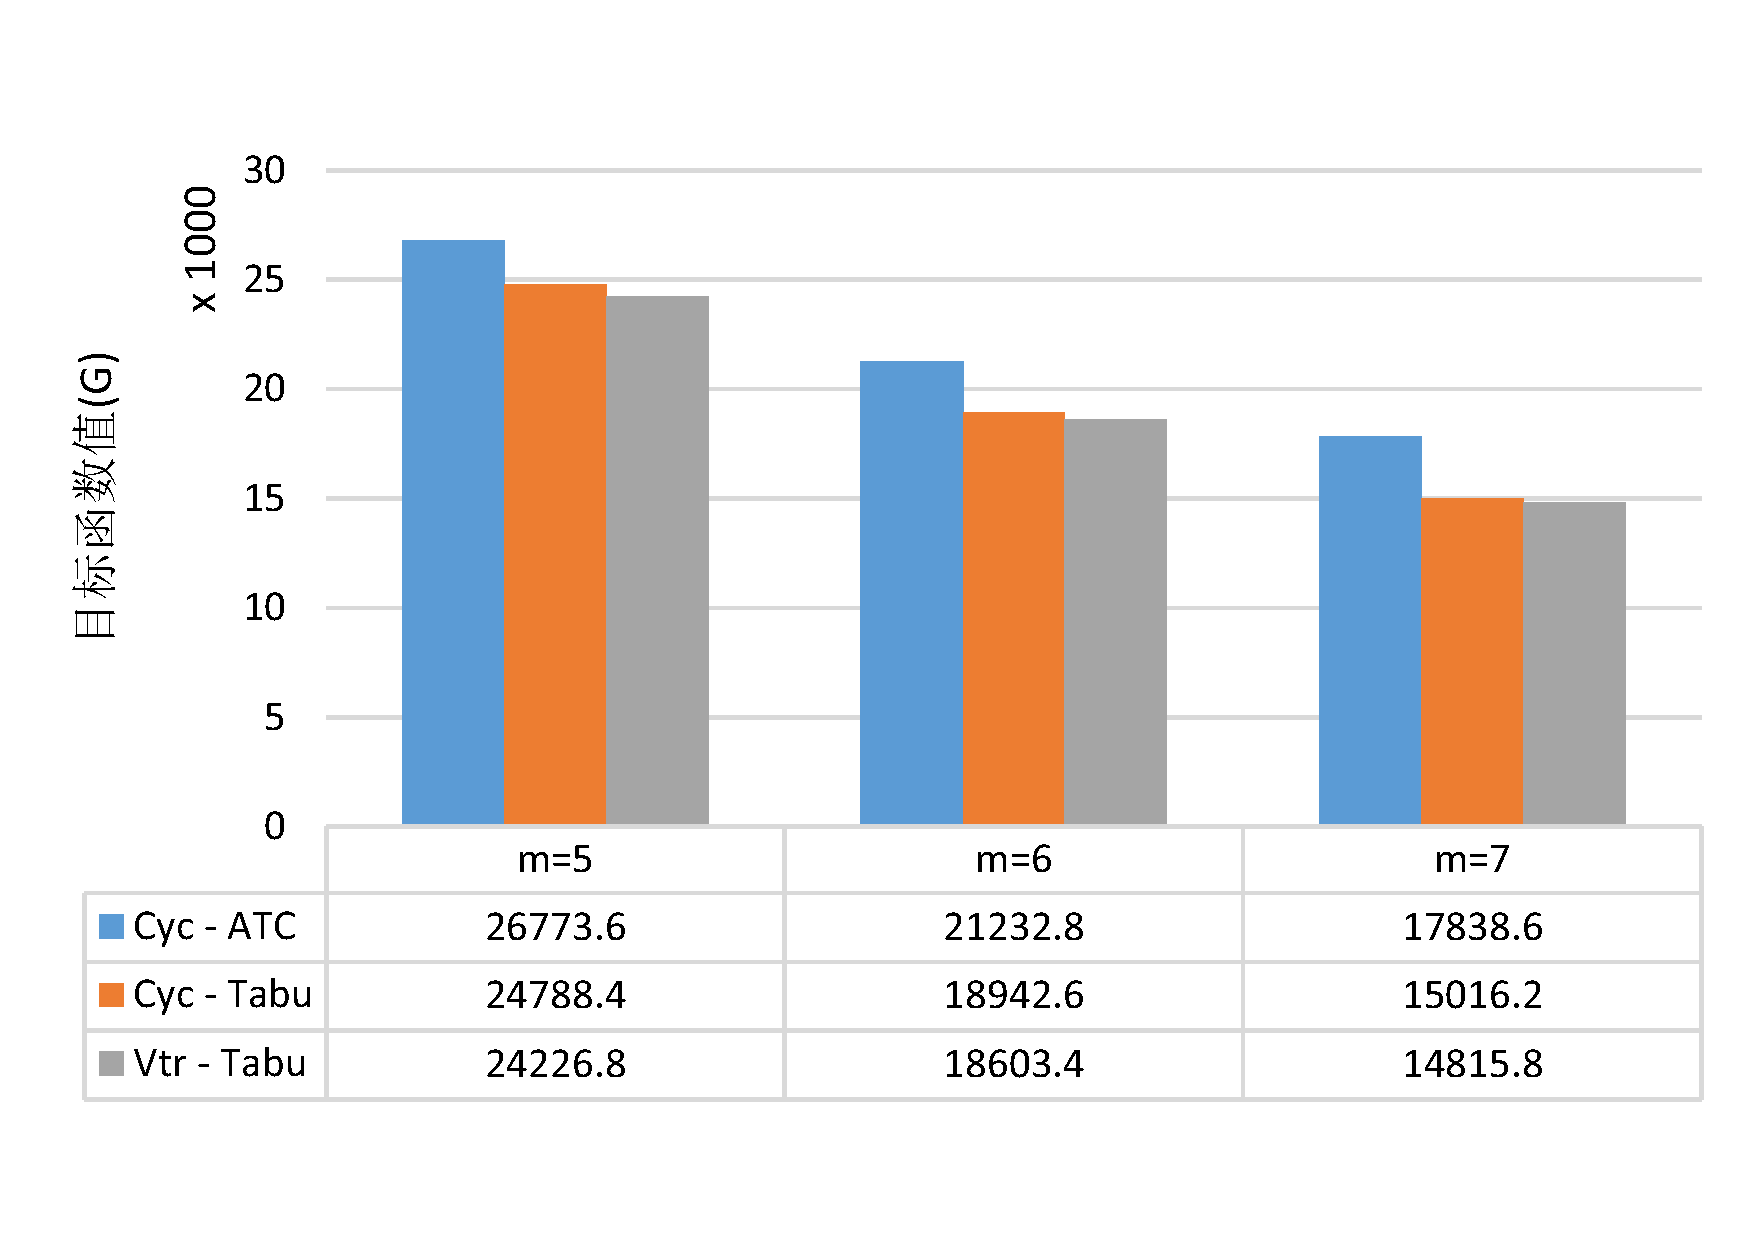
\includegraphics[height = 6cm, angle = -90]{basic_06_50}}
\subfloat[$n = 70$]{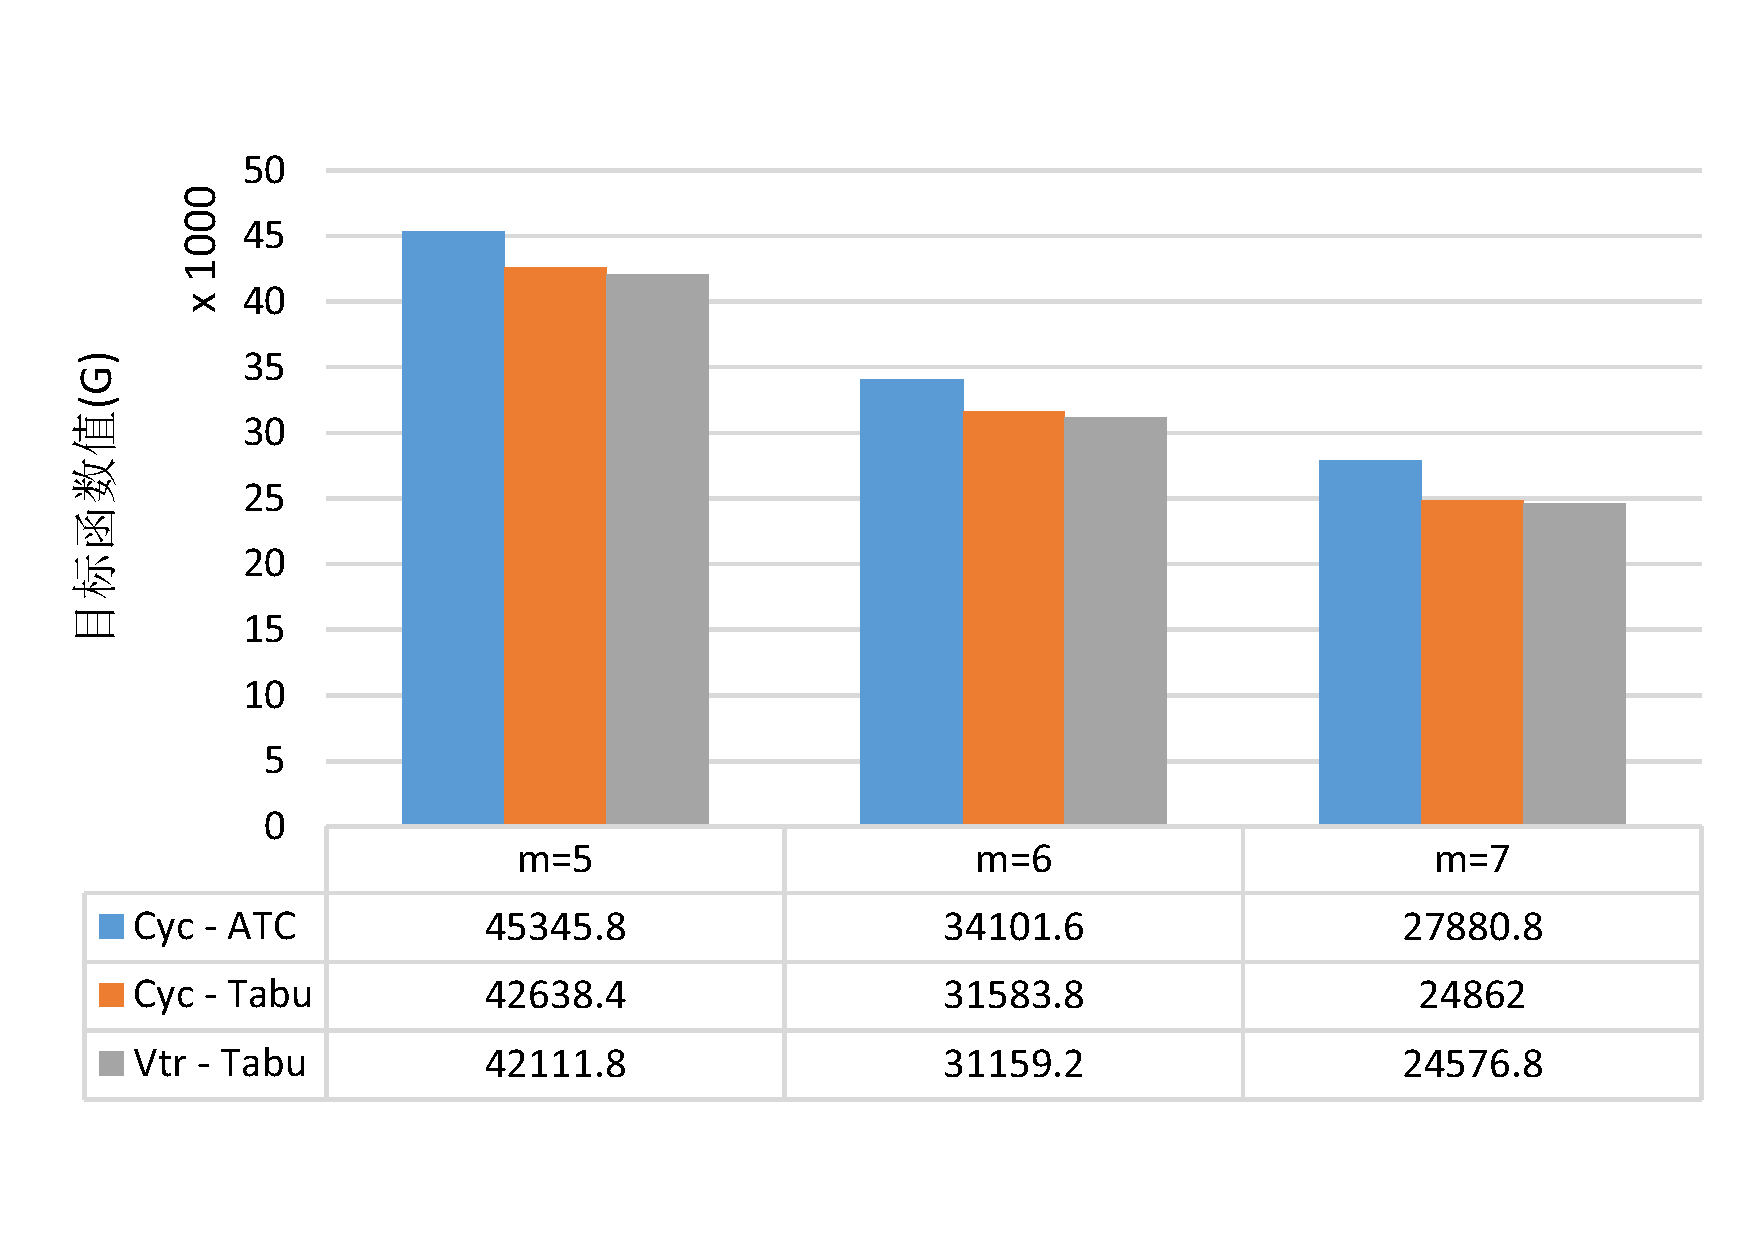
\includegraphics[height = 6cm, angle = -90]{basic_06_70}}\\
\subfloat[$n = 100$]{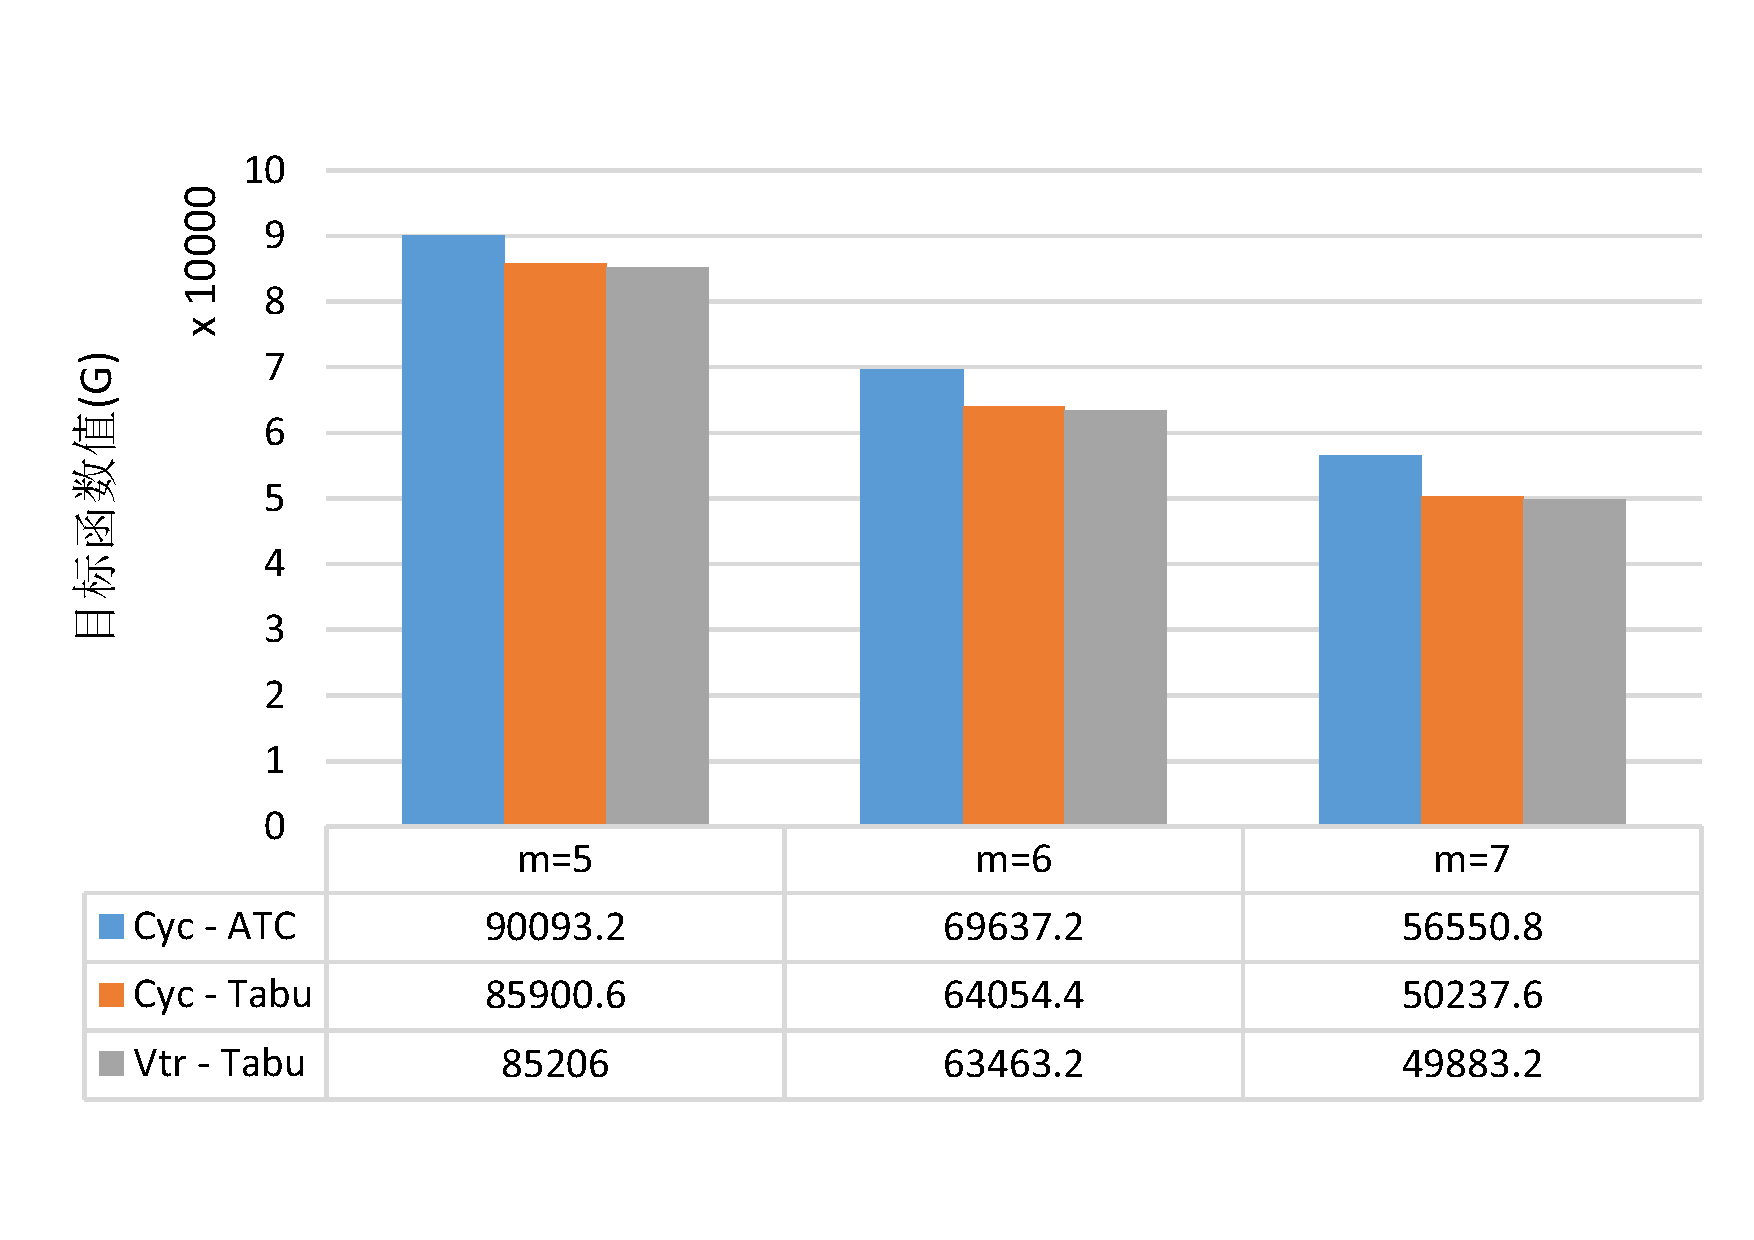
\includegraphics[height = 6cm, angle = -90]{basic_06_100}}
\subfloat[$n = 150$]{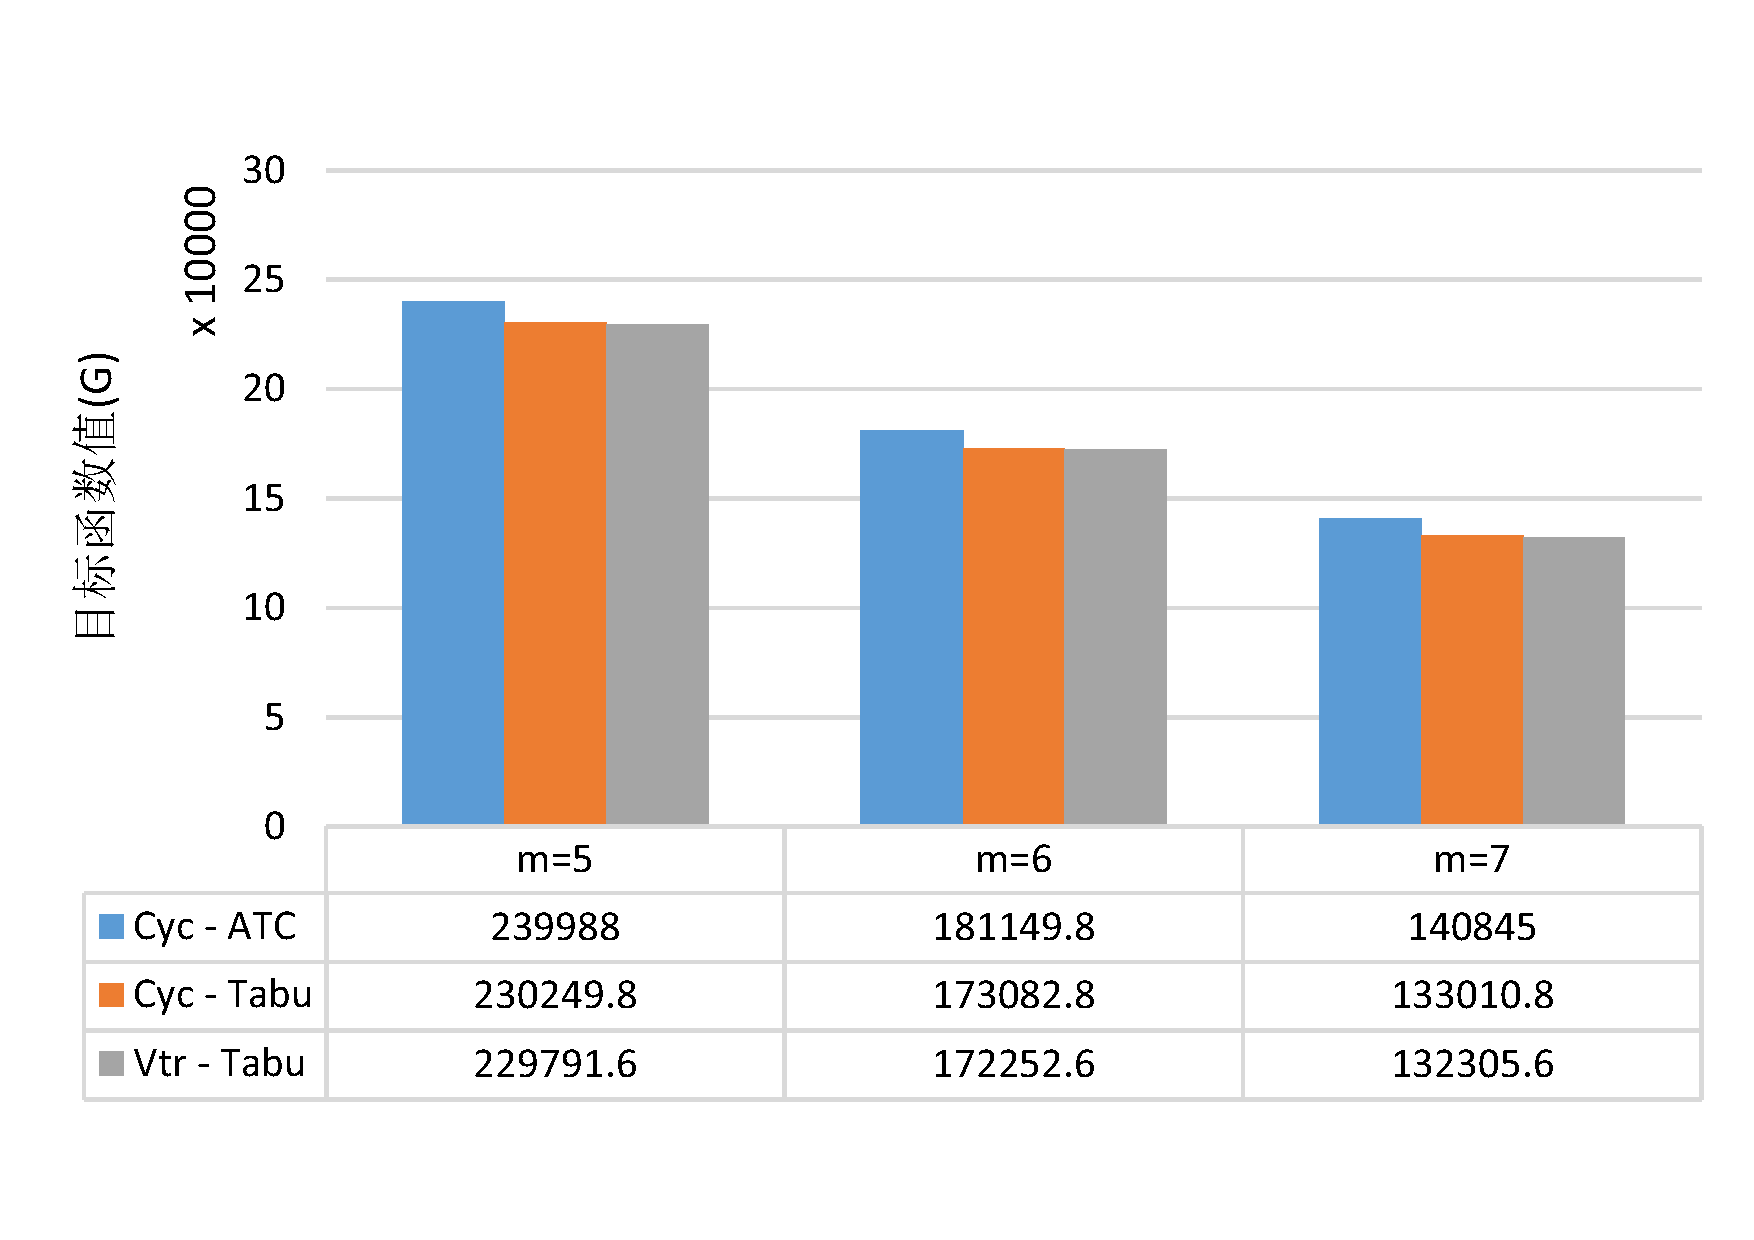
\includegraphics[height = 6cm, angle = -90]{basic_06_150}}
\subfloat[$n = 200$]{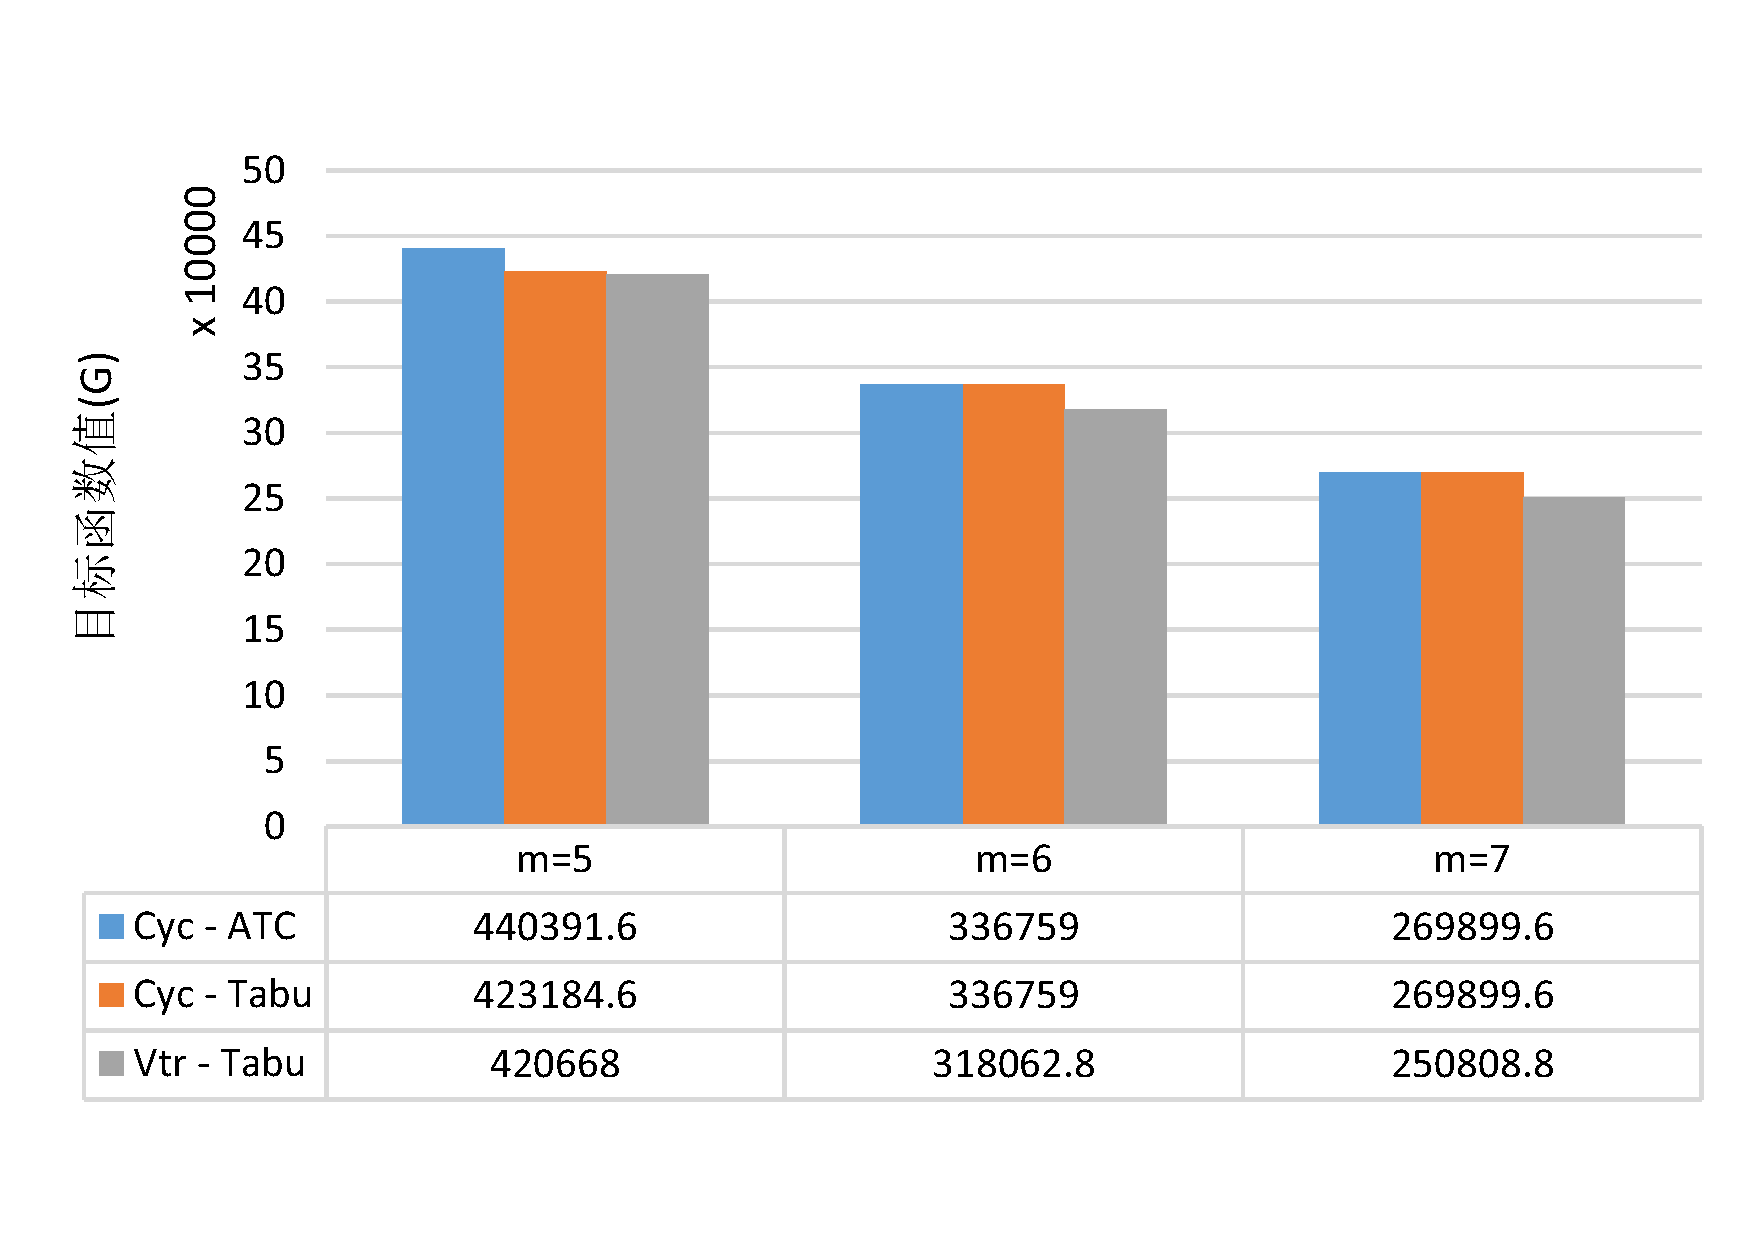
\includegraphics[height = 6cm, angle = -90]{basic_06_200}}
\subfloat[$n = 300$]{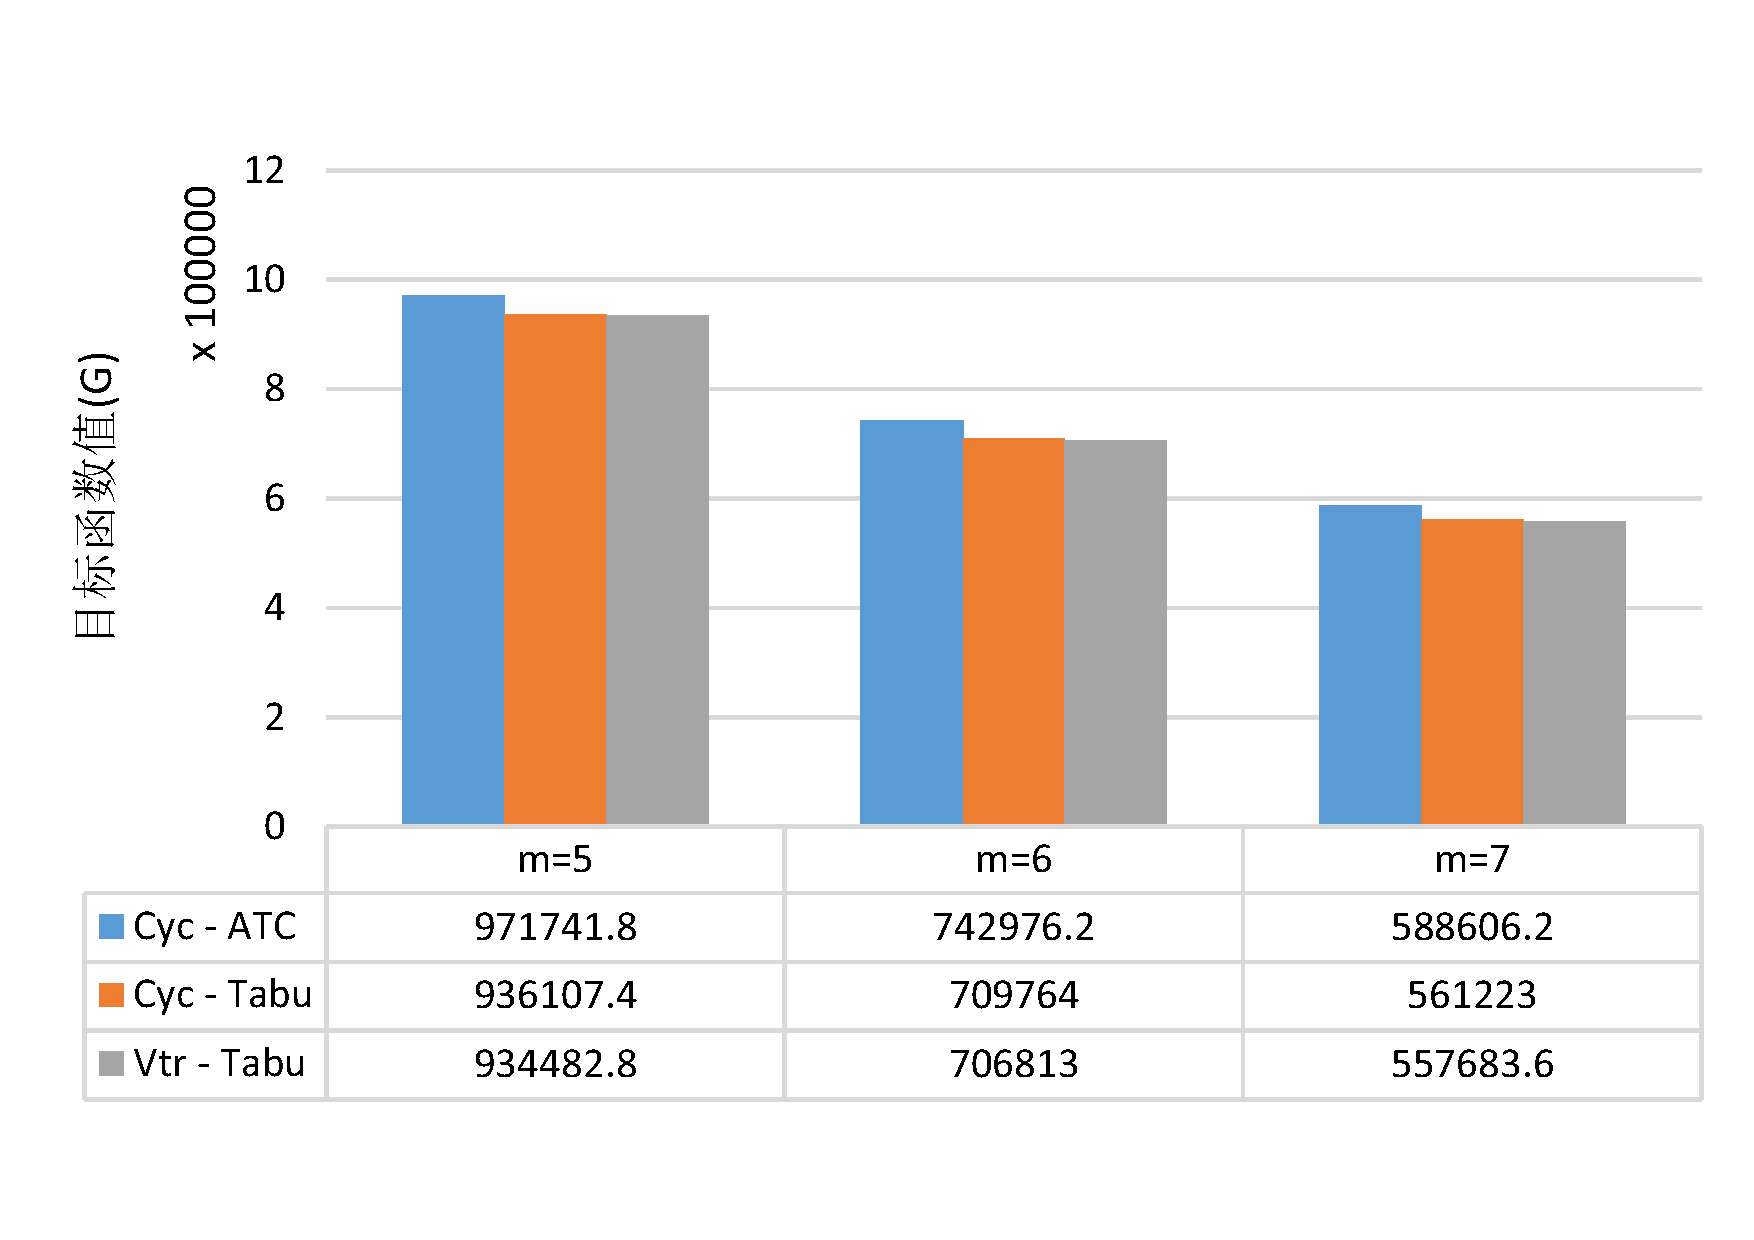
\includegraphics[height = 6cm, angle = -90]{basic_06_300}}\\
\subfloat[$n = 500$]{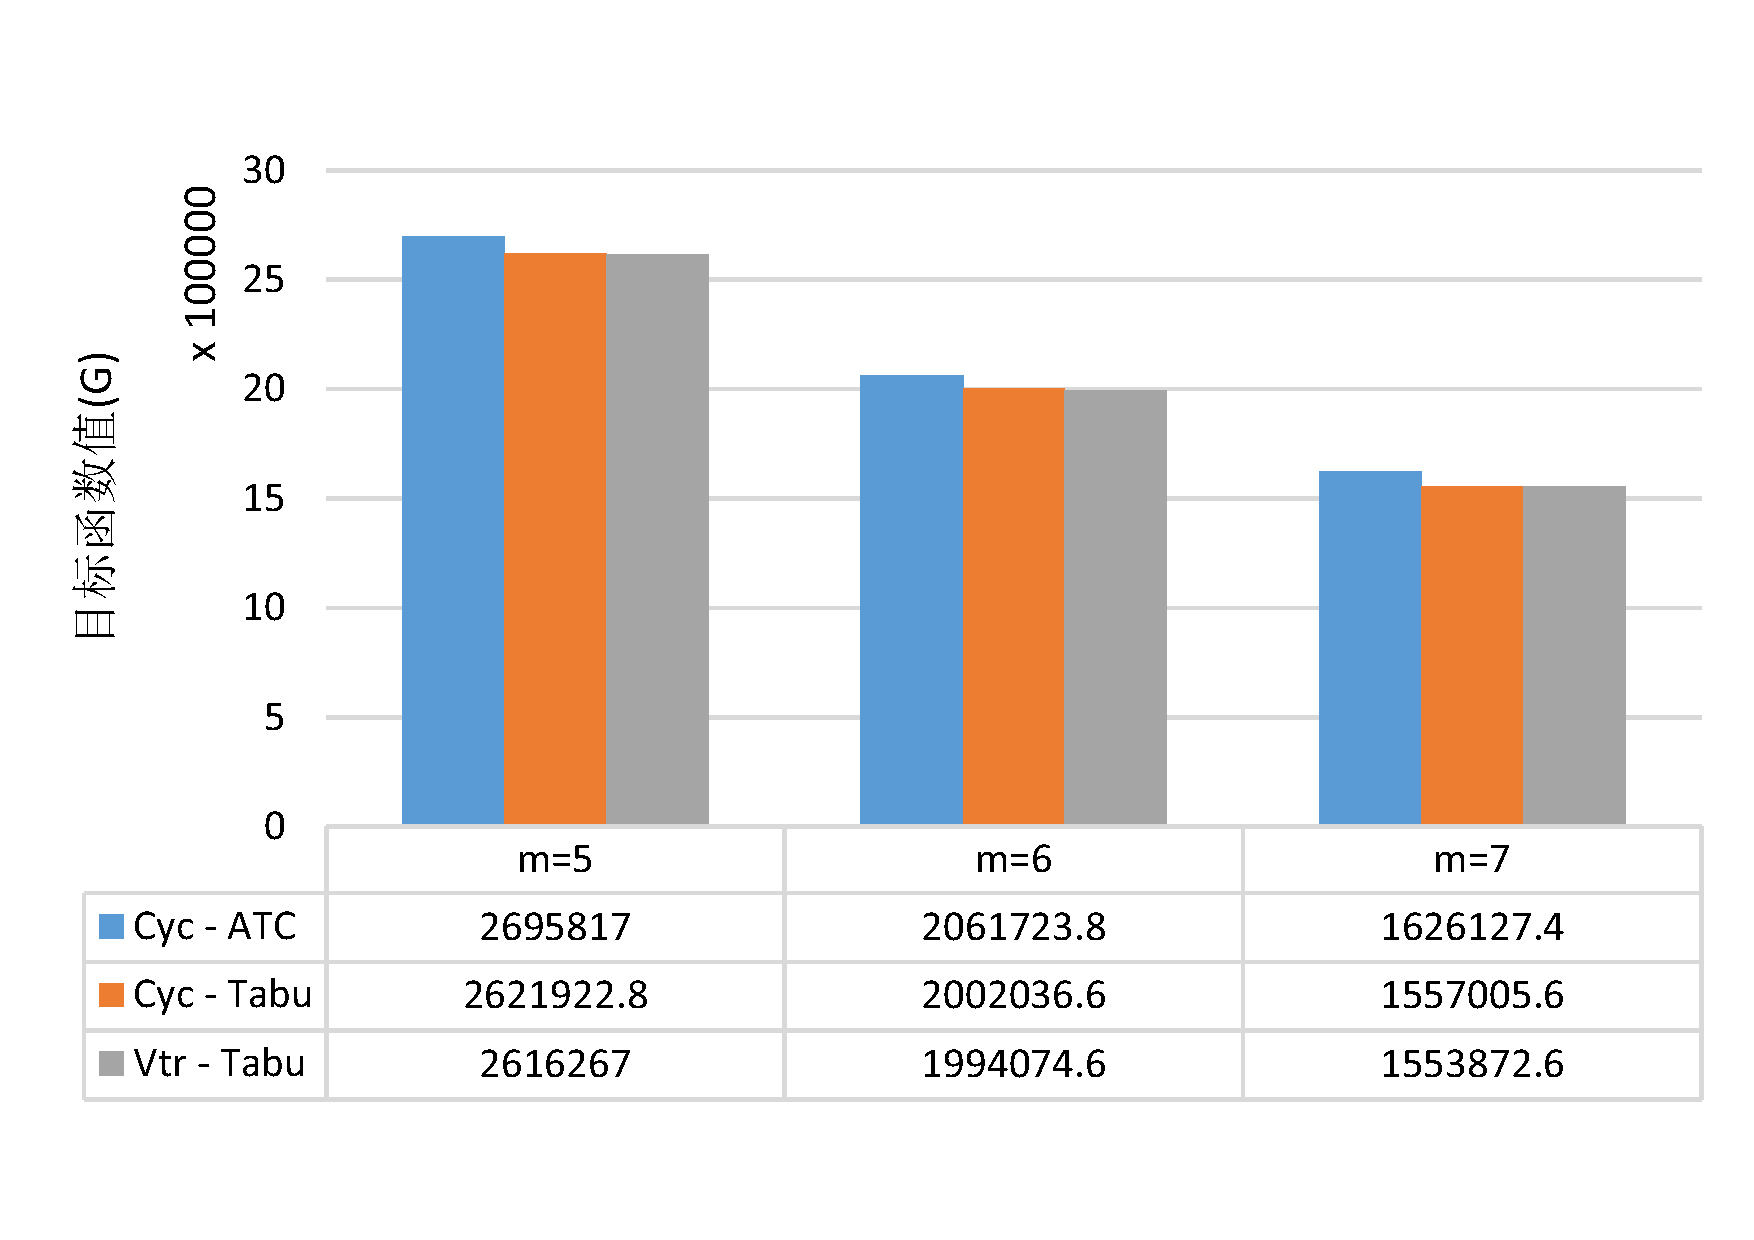
\includegraphics[height = 6cm, angle = -90]{basic_06_500}}
\subfloat[$n = 750$]{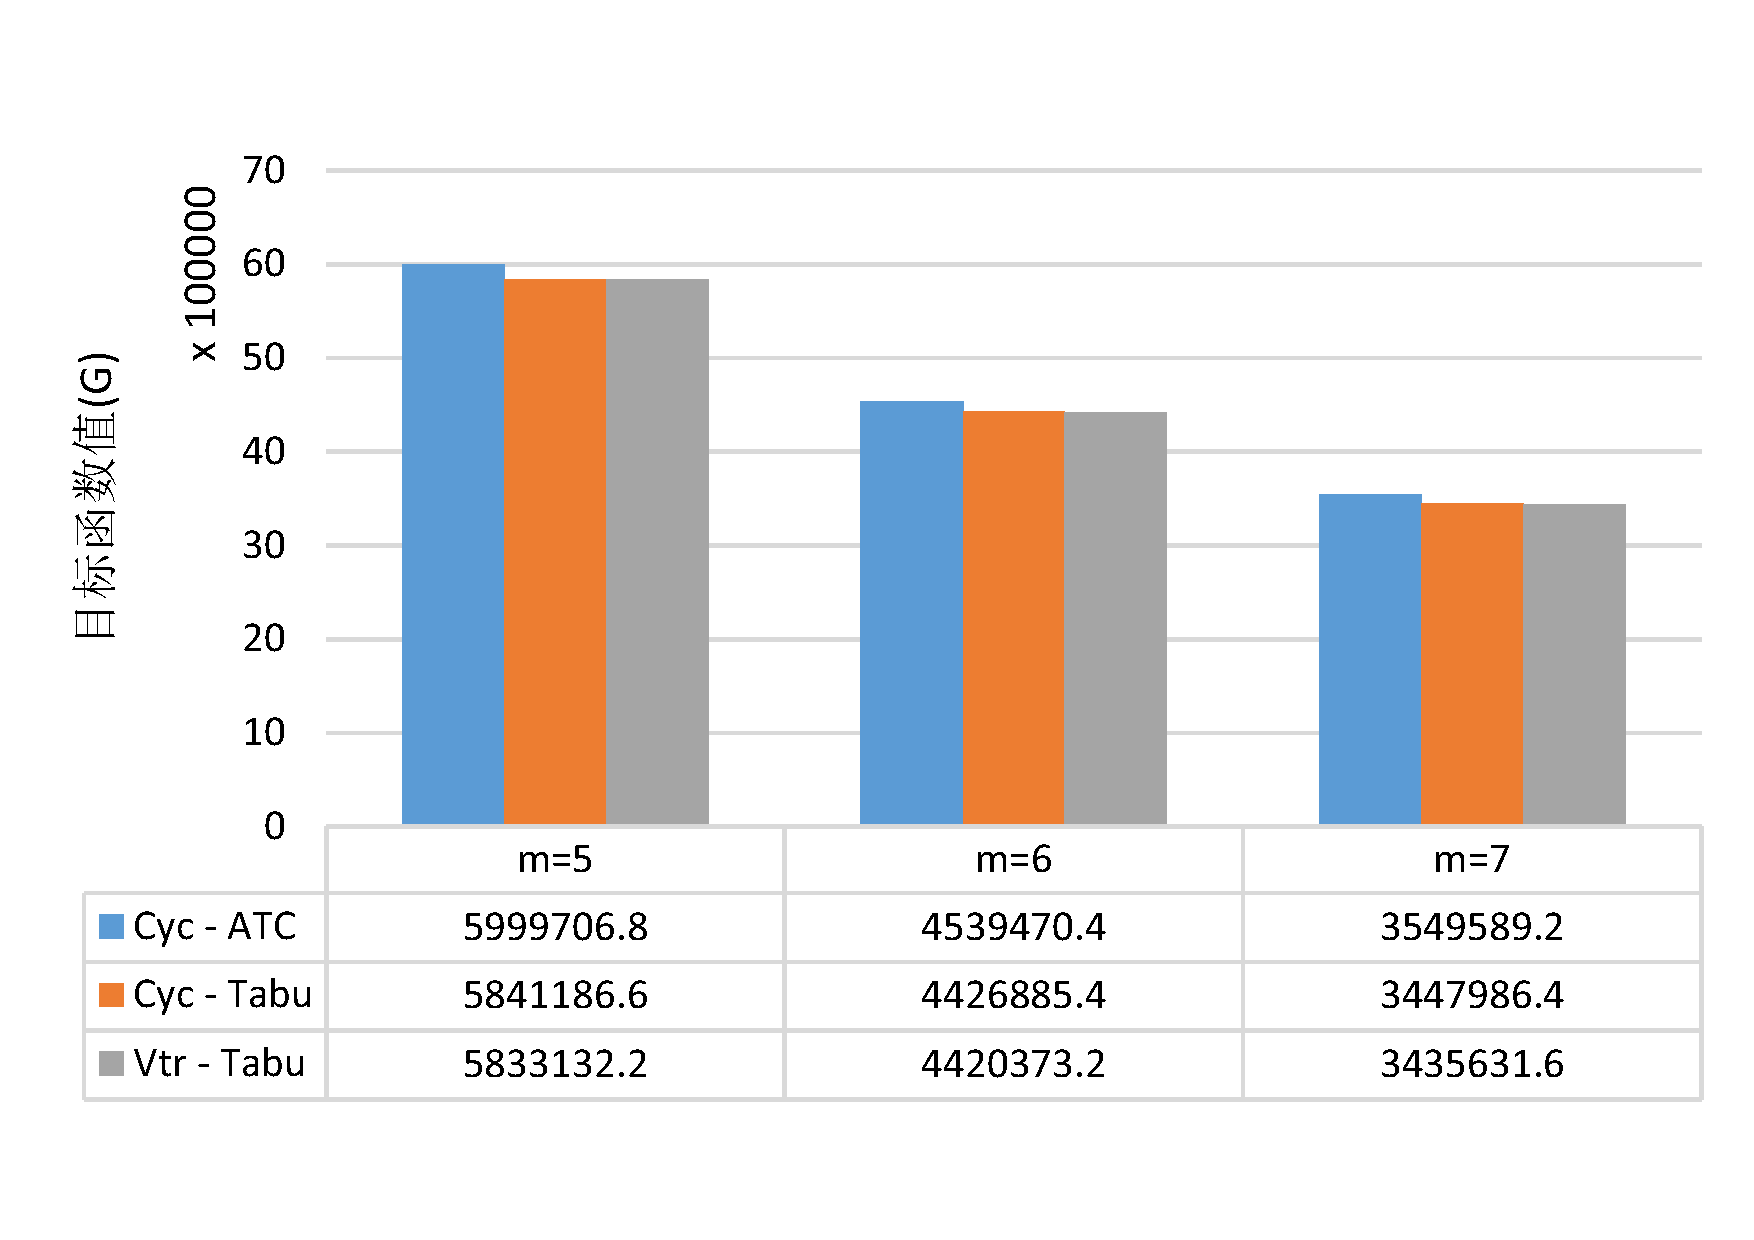
\includegraphics[height = 6cm, angle = -90]{basic_06_750}}
\subfloat[$n = 1000$]{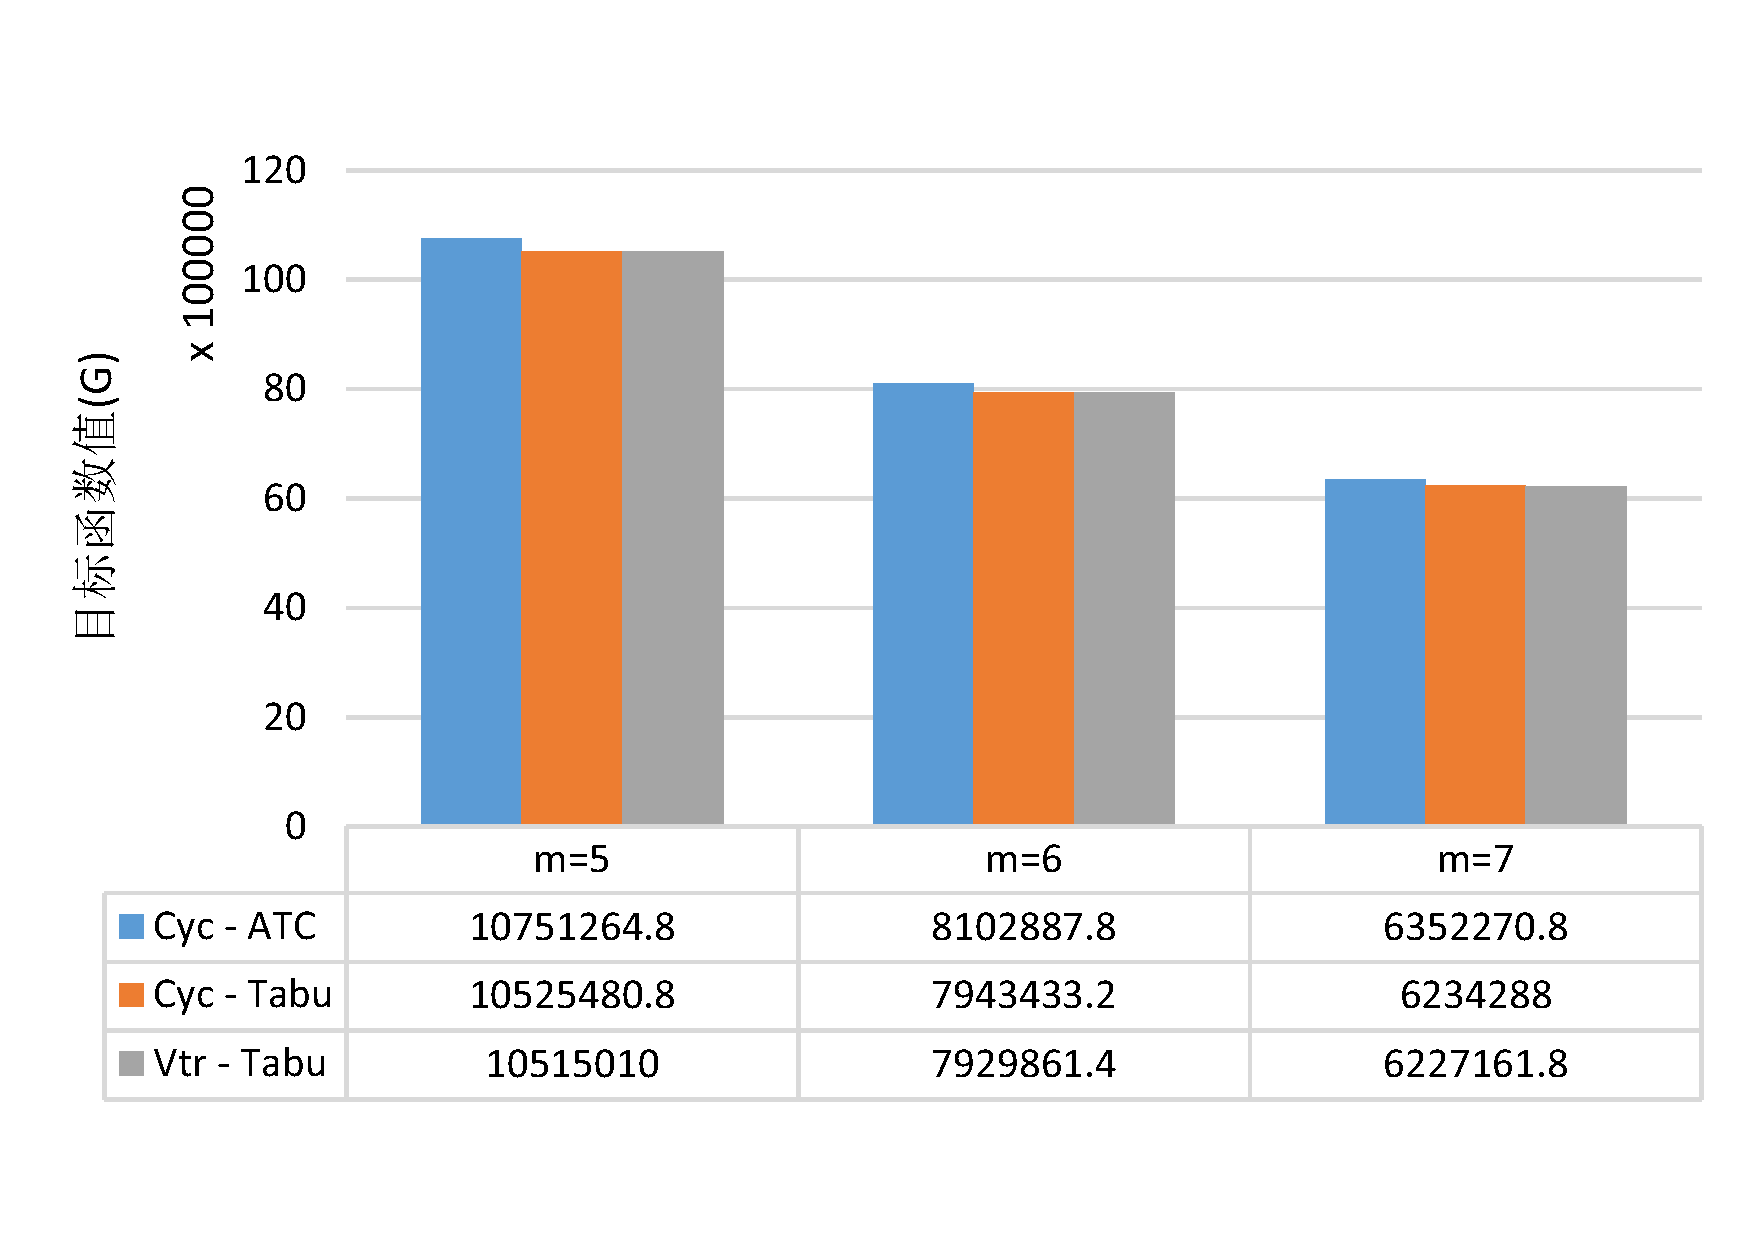
\includegraphics[height = 6cm, angle = -90]{basic_06_1000}}
\caption{\label{fig:result3}模型$1$的Cyc -- ATC、Cyc -- Tabu、Vtr -- Tabu 算法求解目标函数值比较$(\lambda_1 = 0.6)$}
\end{sidewaysfigure}

\begin{sidewaysfigure}
\centering
\subfloat[$n = 20$]{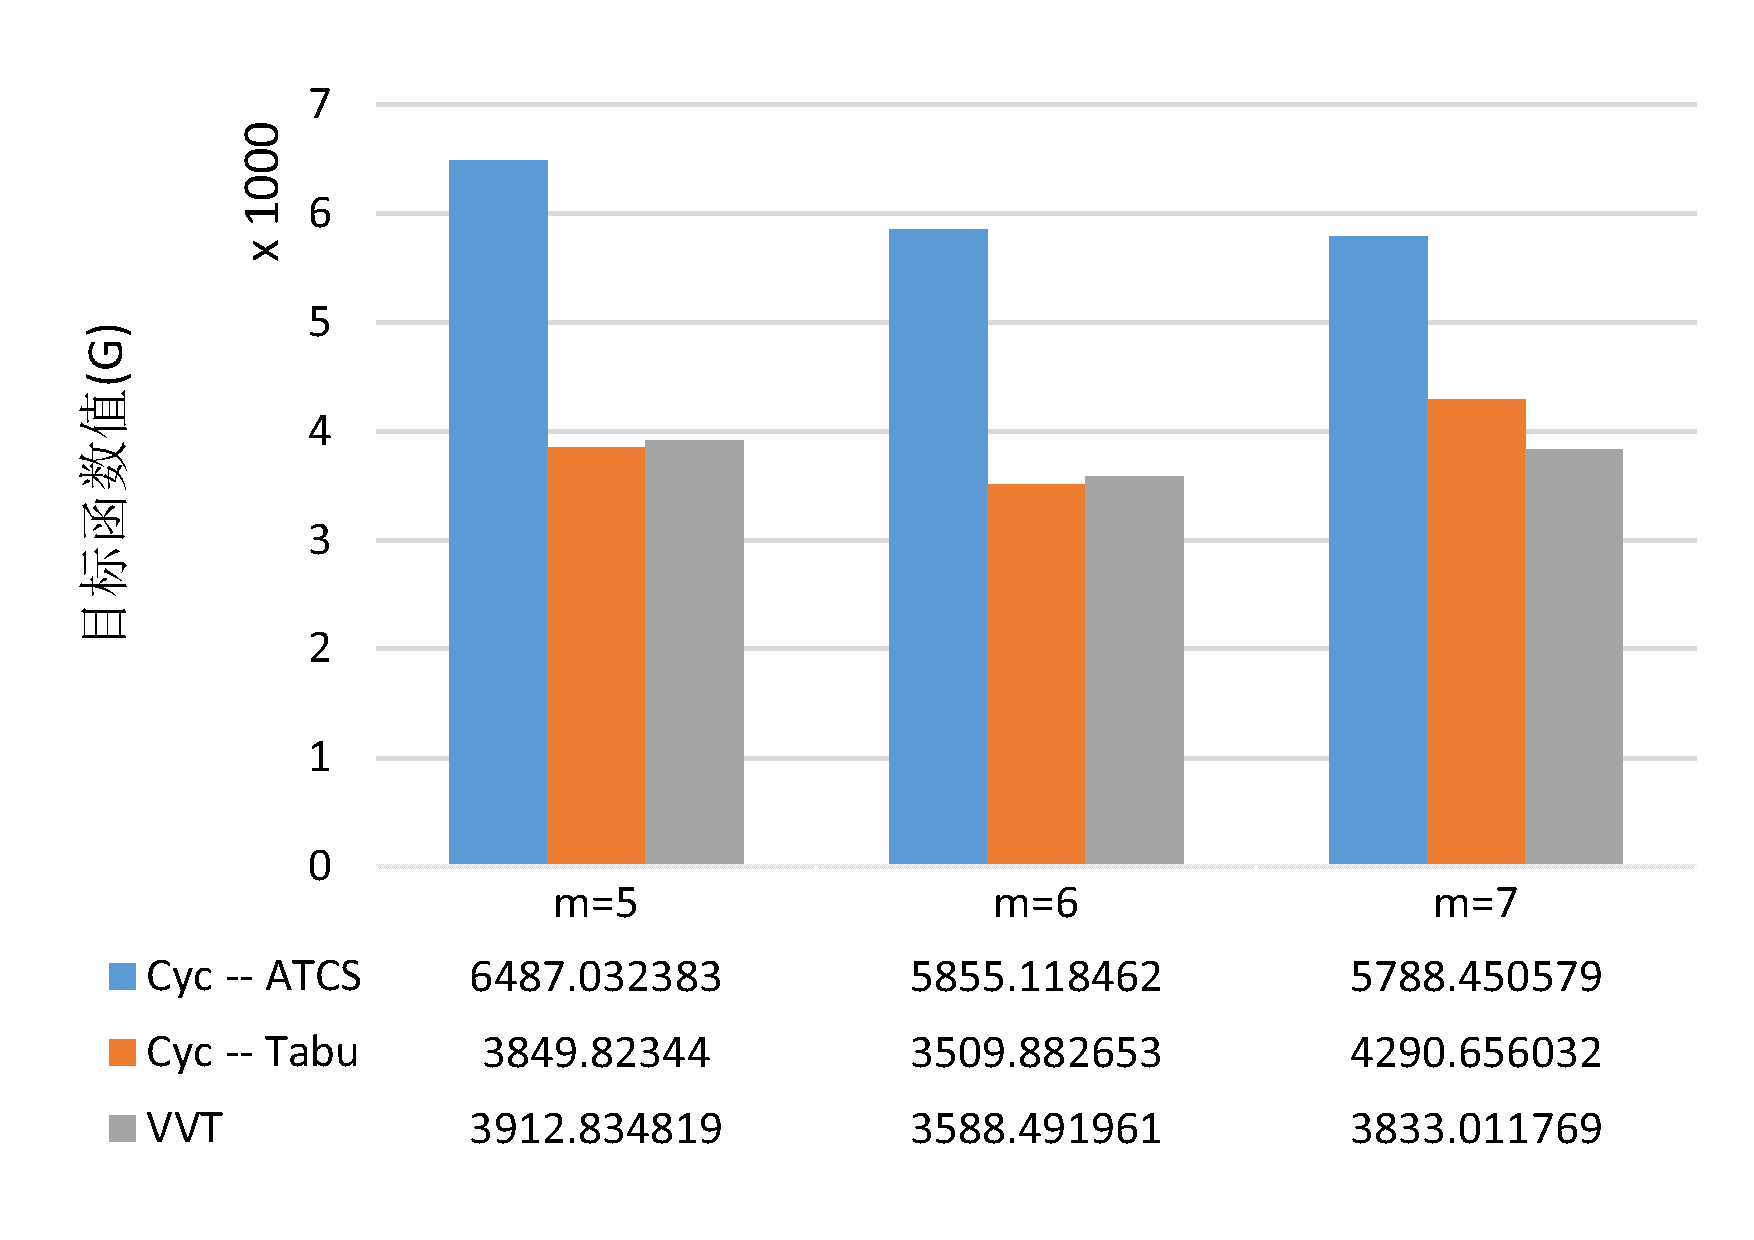
\includegraphics[height = 6cm, angle = -90]{continue_04_20}}
\subfloat[$n = 30$]{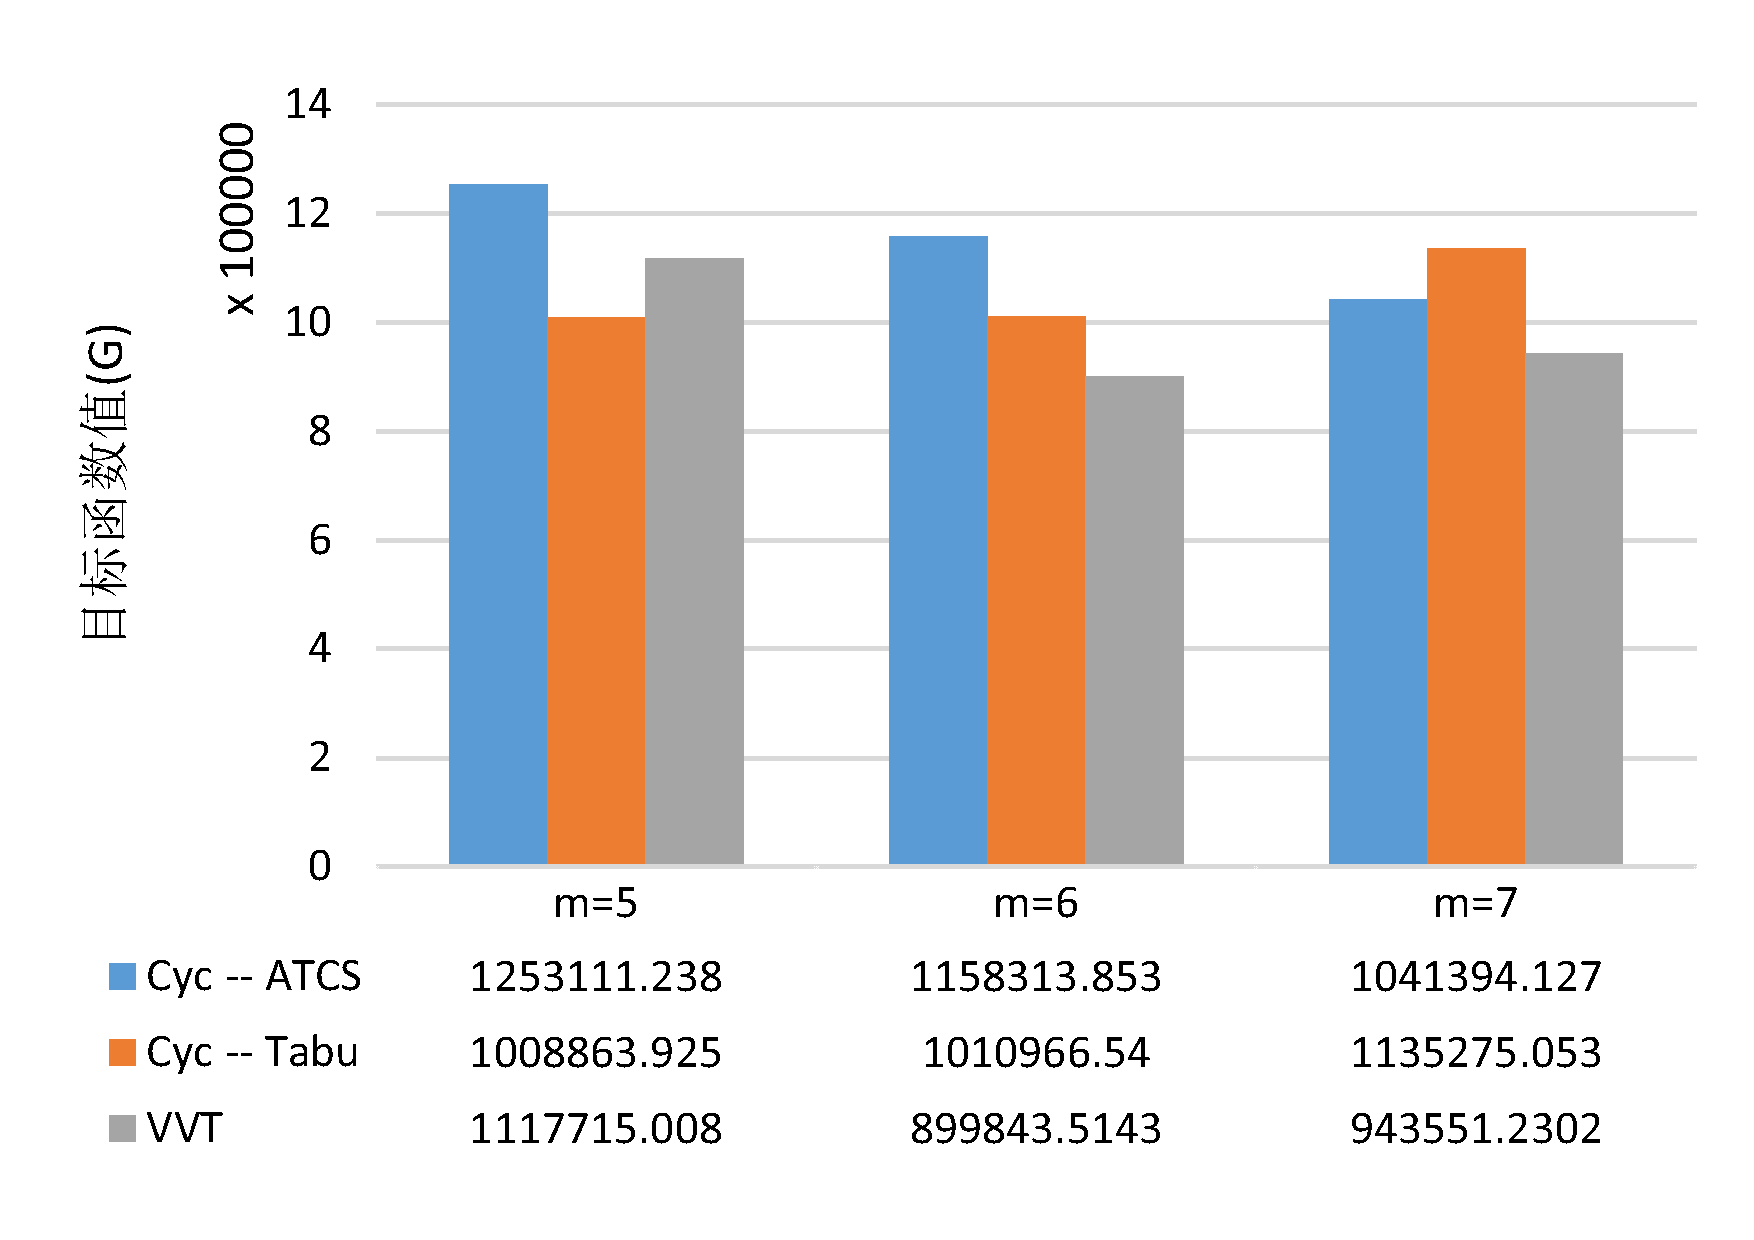
\includegraphics[height = 6cm, angle = -90]{continue_04_300}}
\subfloat[$n = 50$]{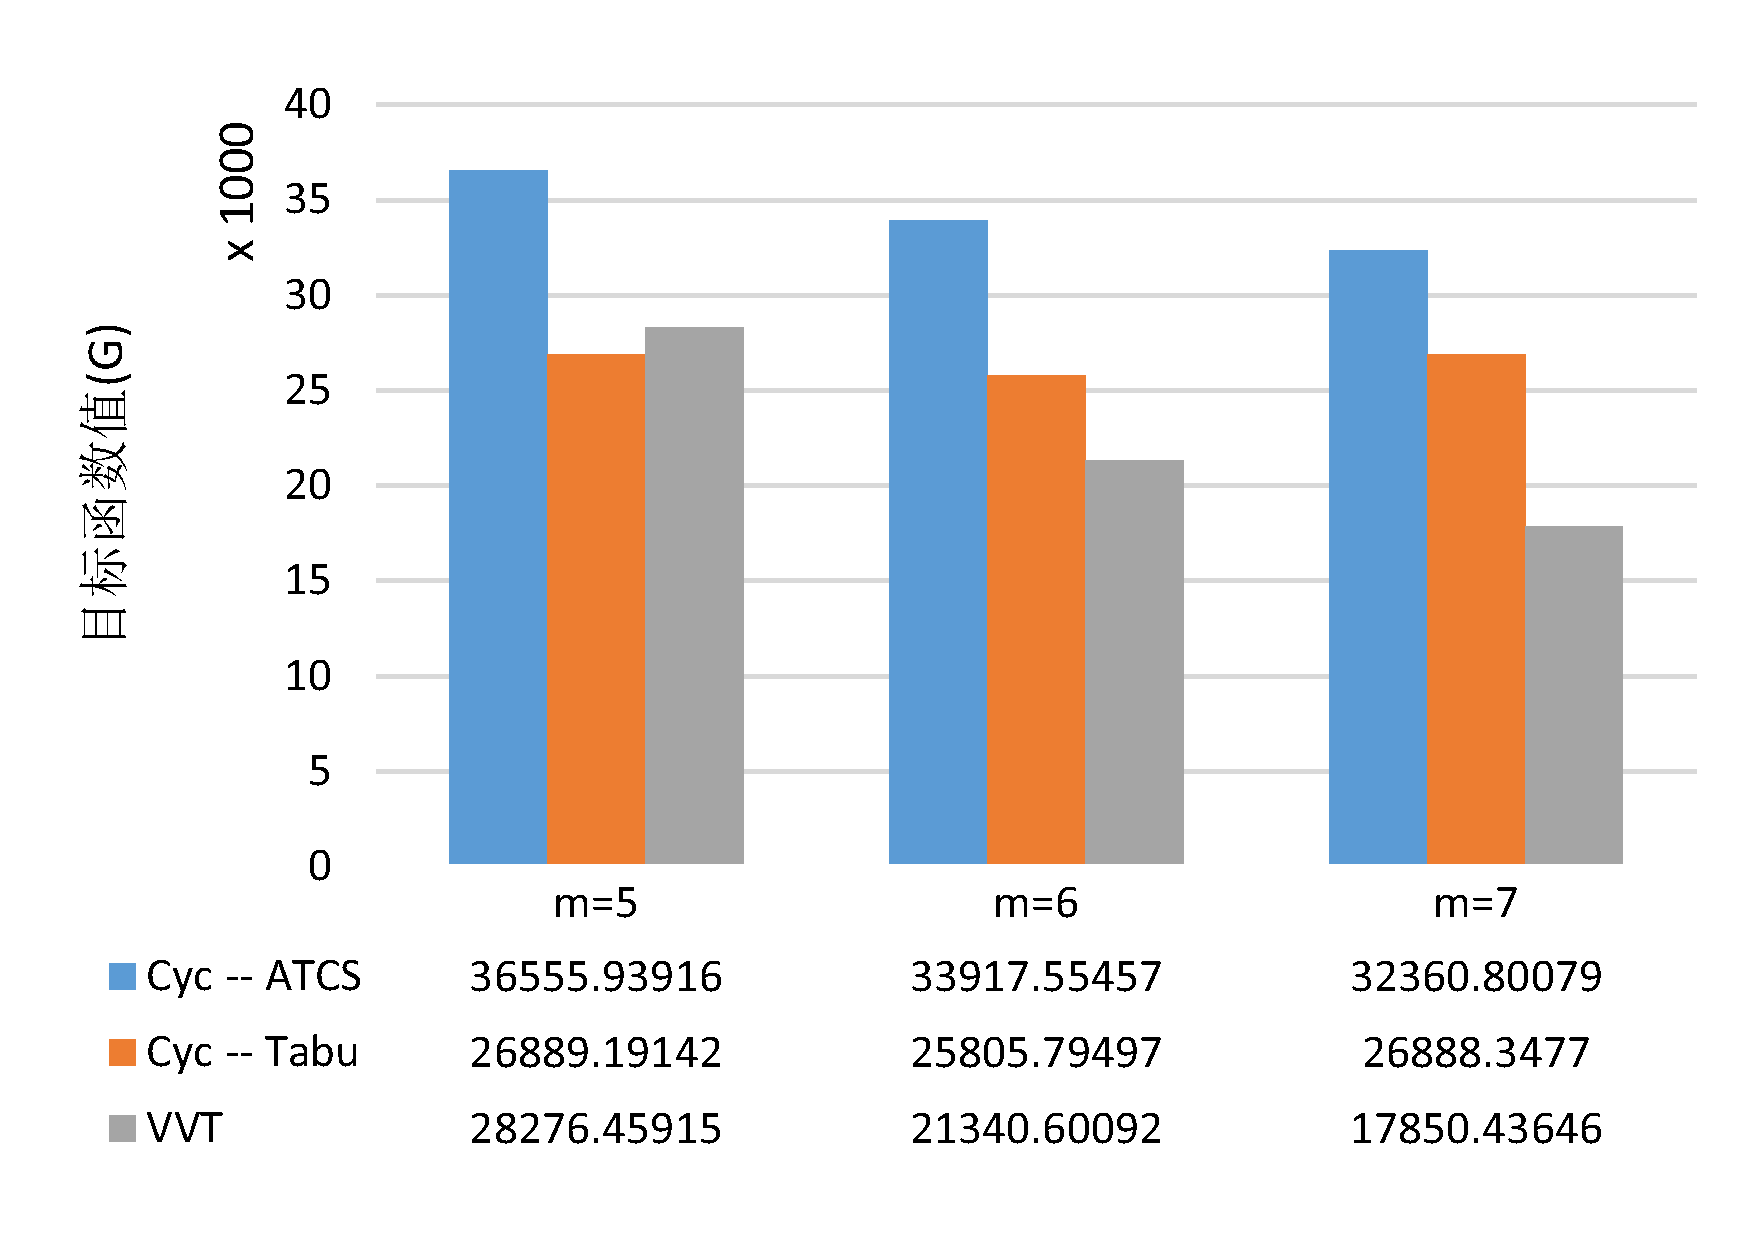
\includegraphics[height = 6cm, angle = -90]{continue_04_50}}
\subfloat[$n = 70$]{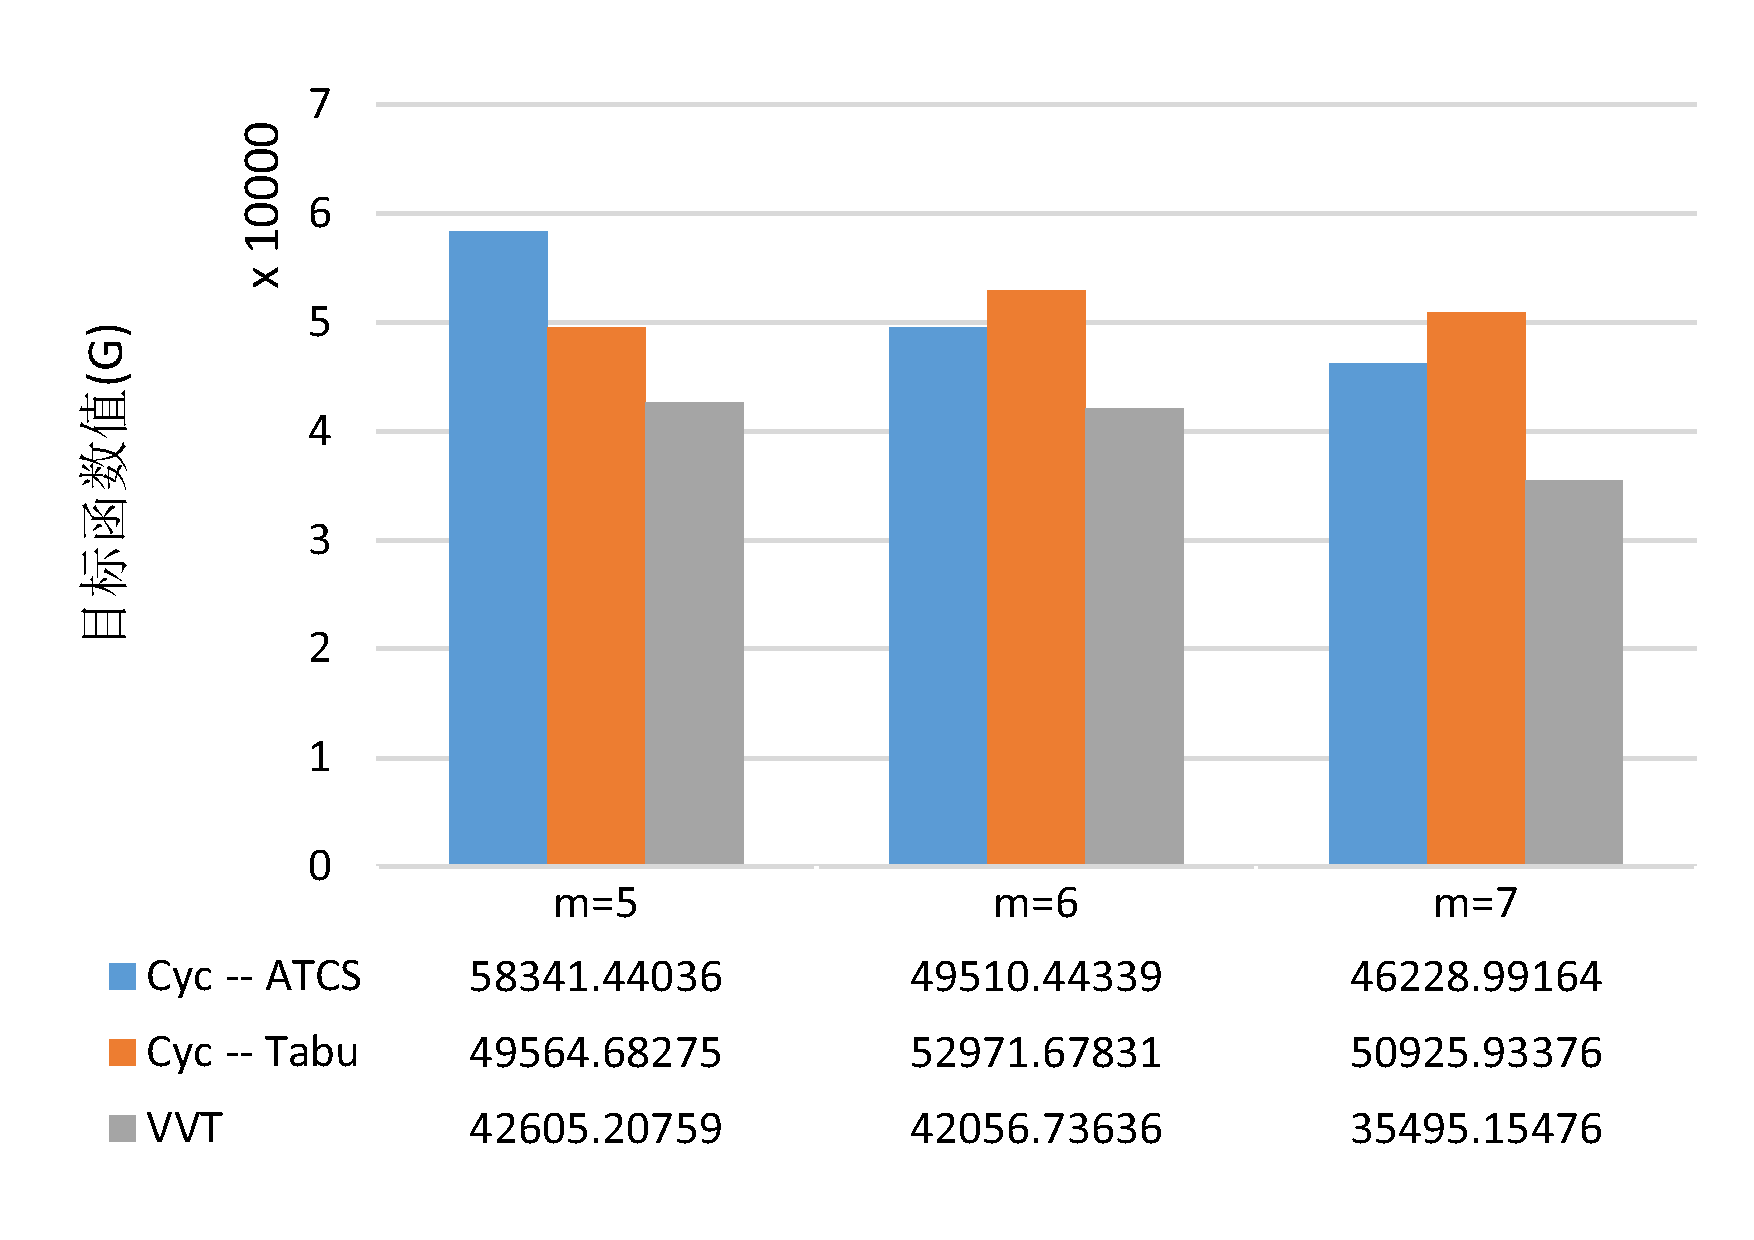
\includegraphics[height = 6cm, angle = -90]{continue_04_70}}\\
\subfloat[$n = 100$]{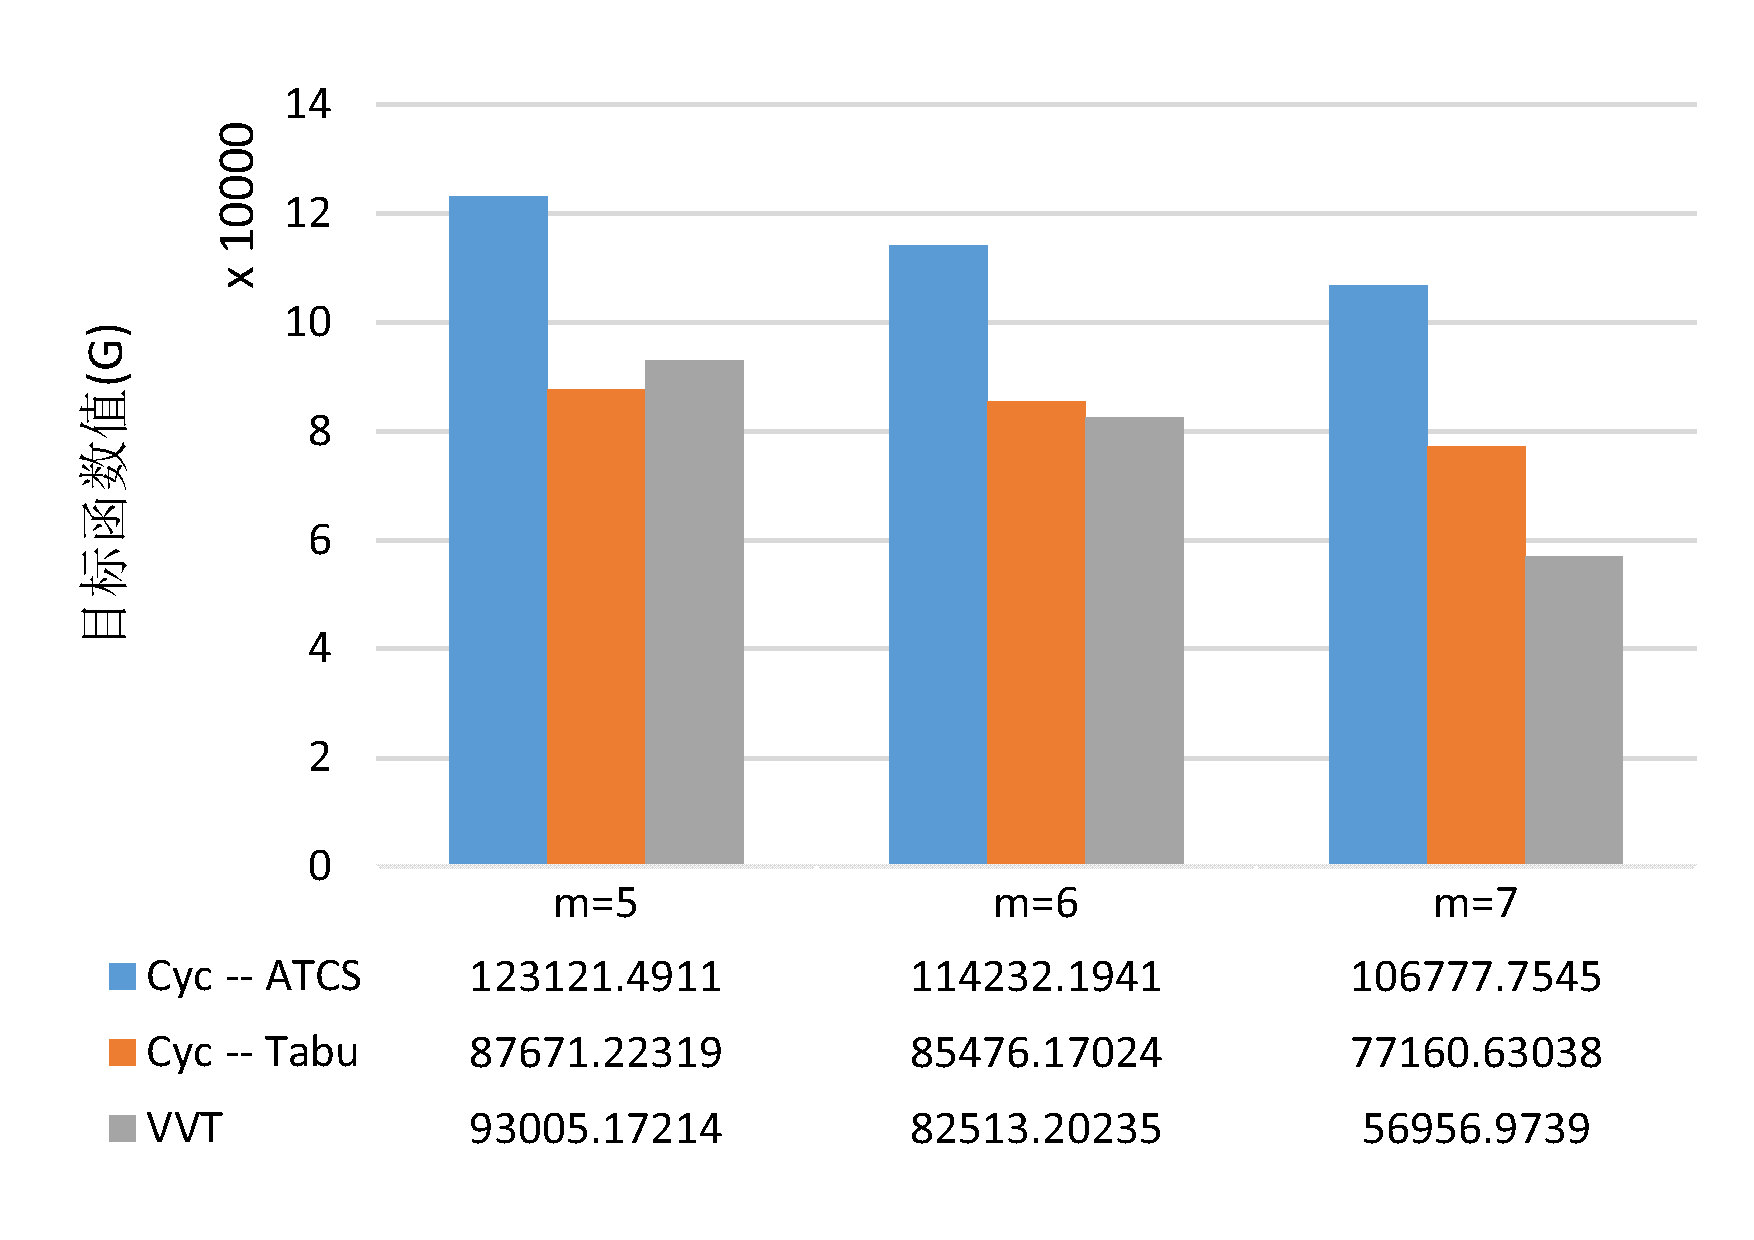
\includegraphics[height = 6cm, angle = -90]{continue_04_100}}
\subfloat[$n = 150$]{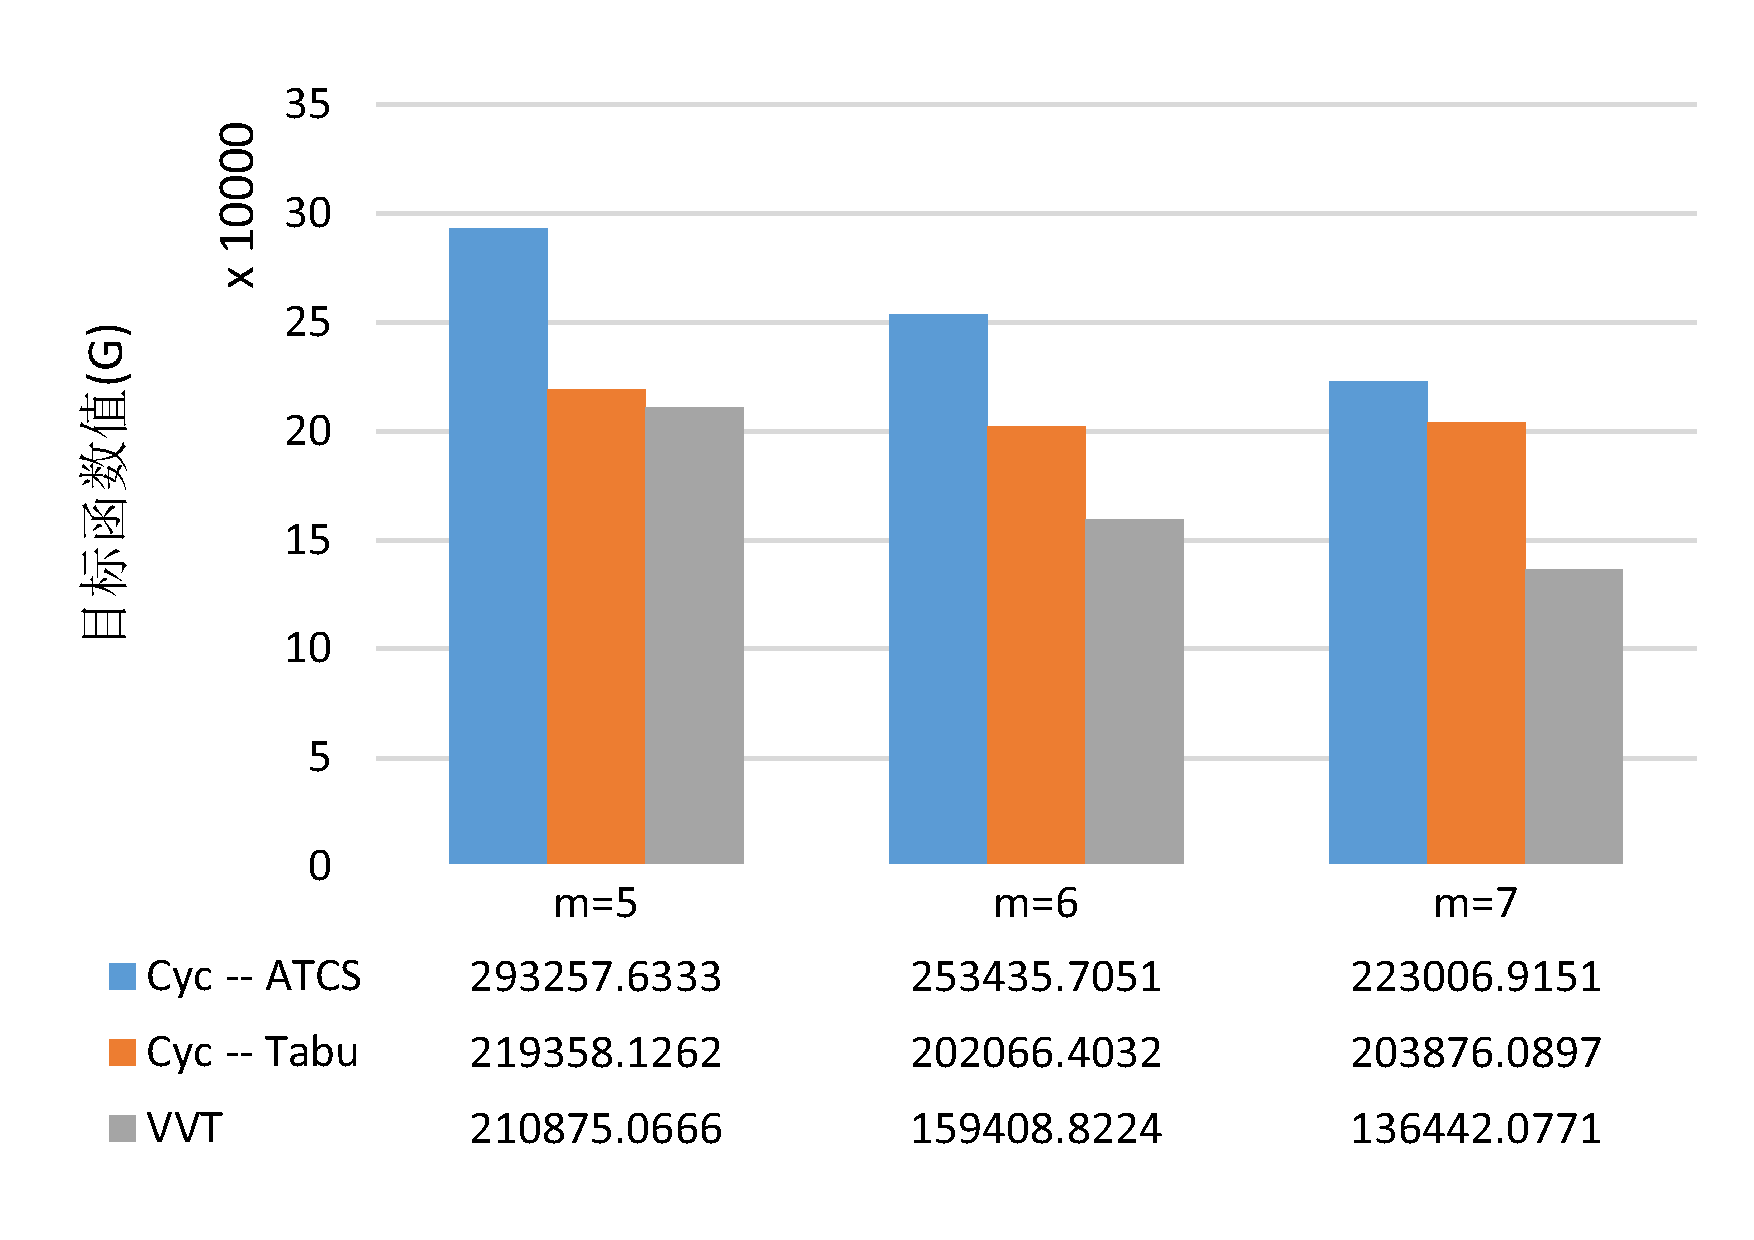
\includegraphics[height = 6cm, angle = -90]{continue_04_150}}
\subfloat[$n = 200$]{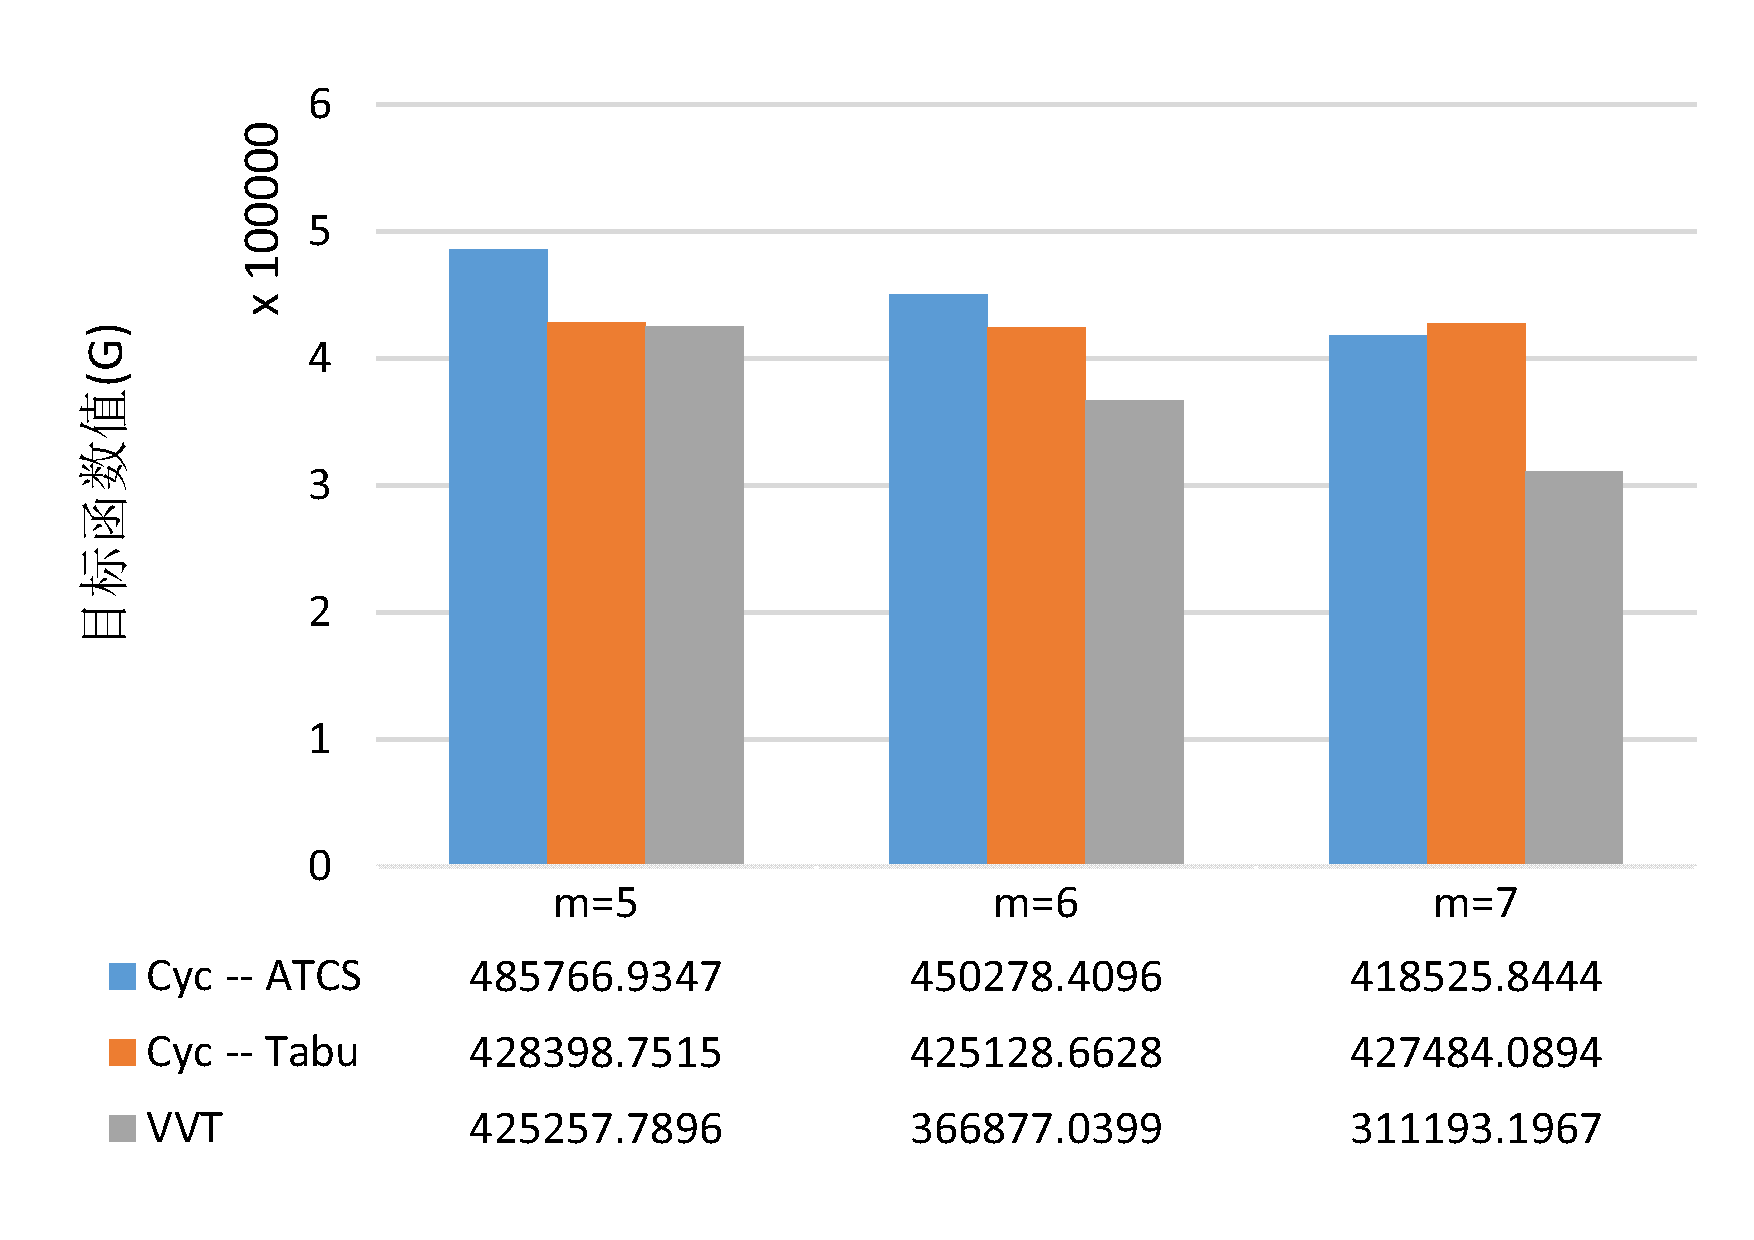
\includegraphics[height = 6cm, angle = -90]{continue_04_200}}
\subfloat[$n = 300$]{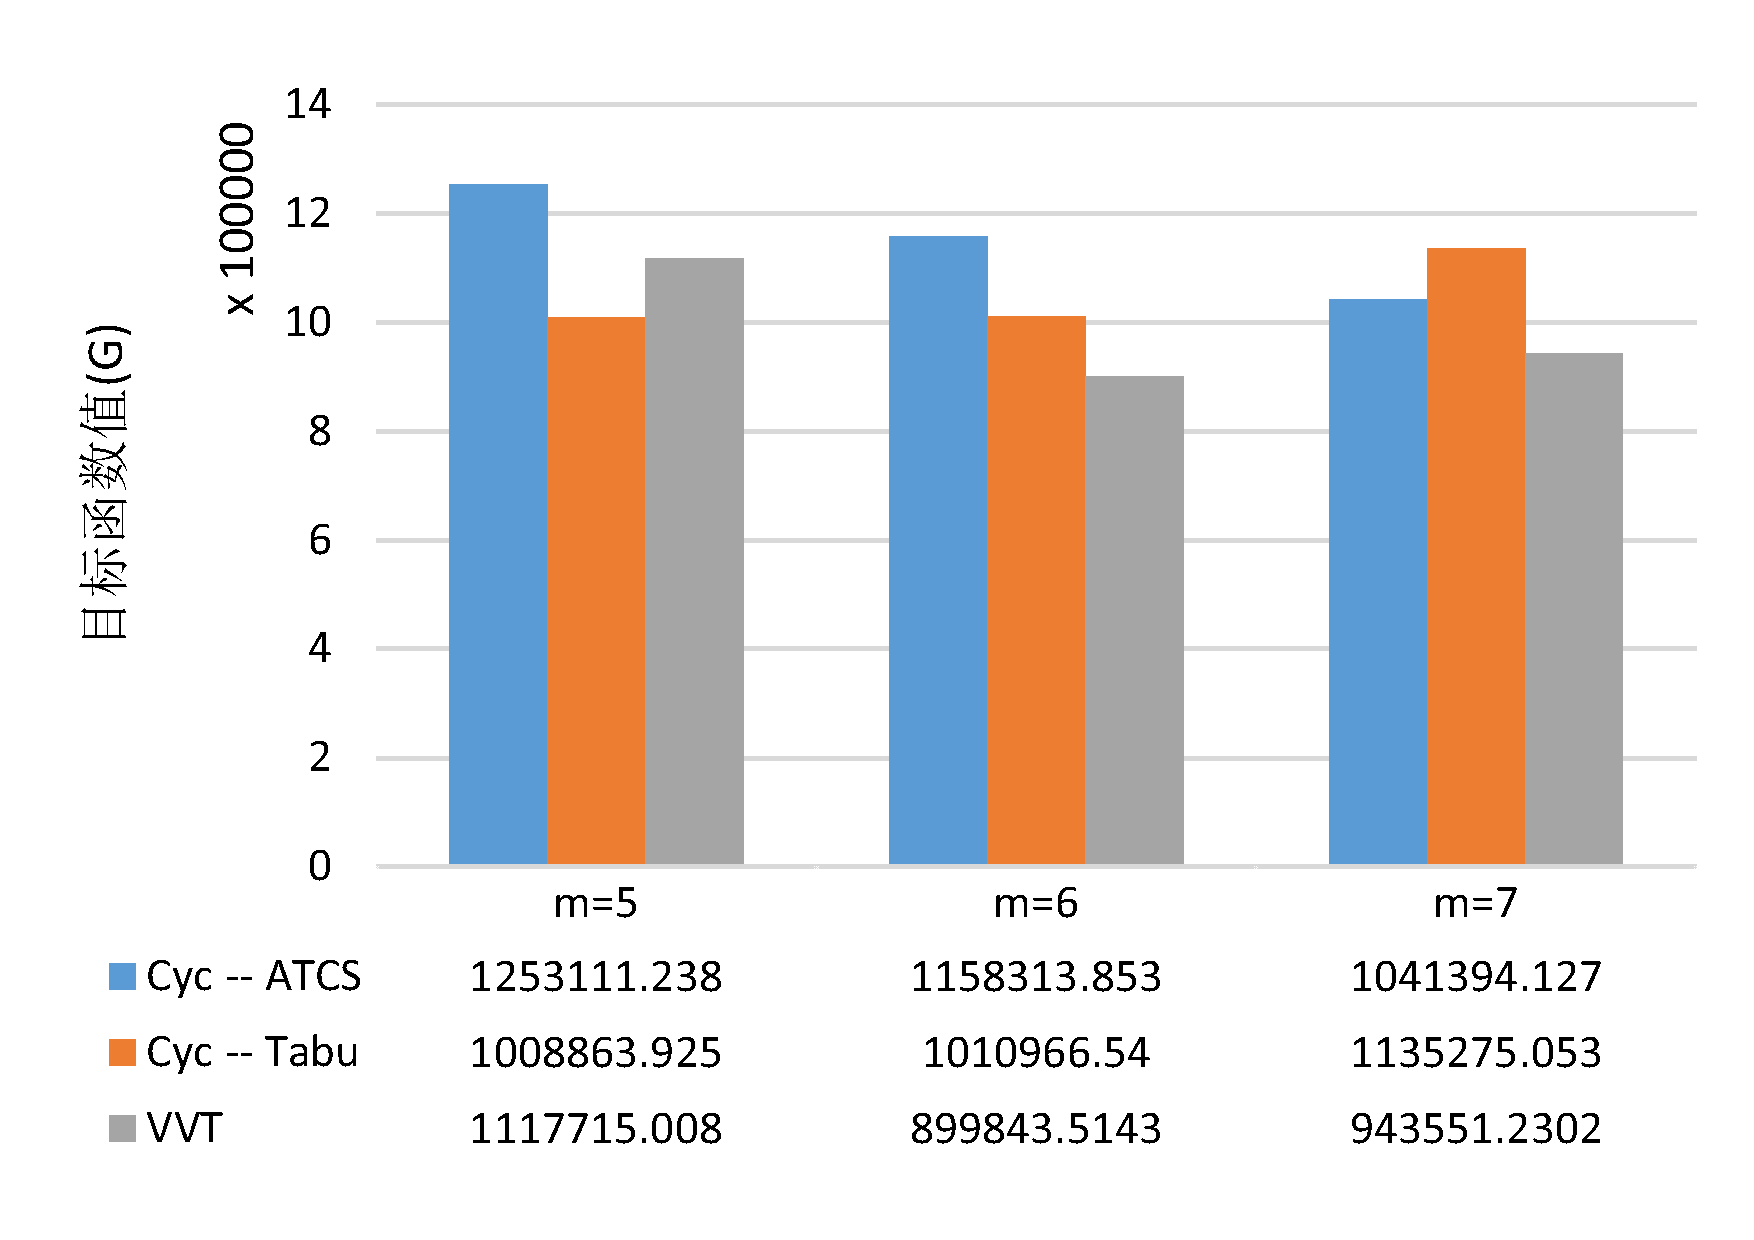
\includegraphics[height = 6cm, angle = -90]{continue_04_300}}\\
\subfloat[$n = 500$]{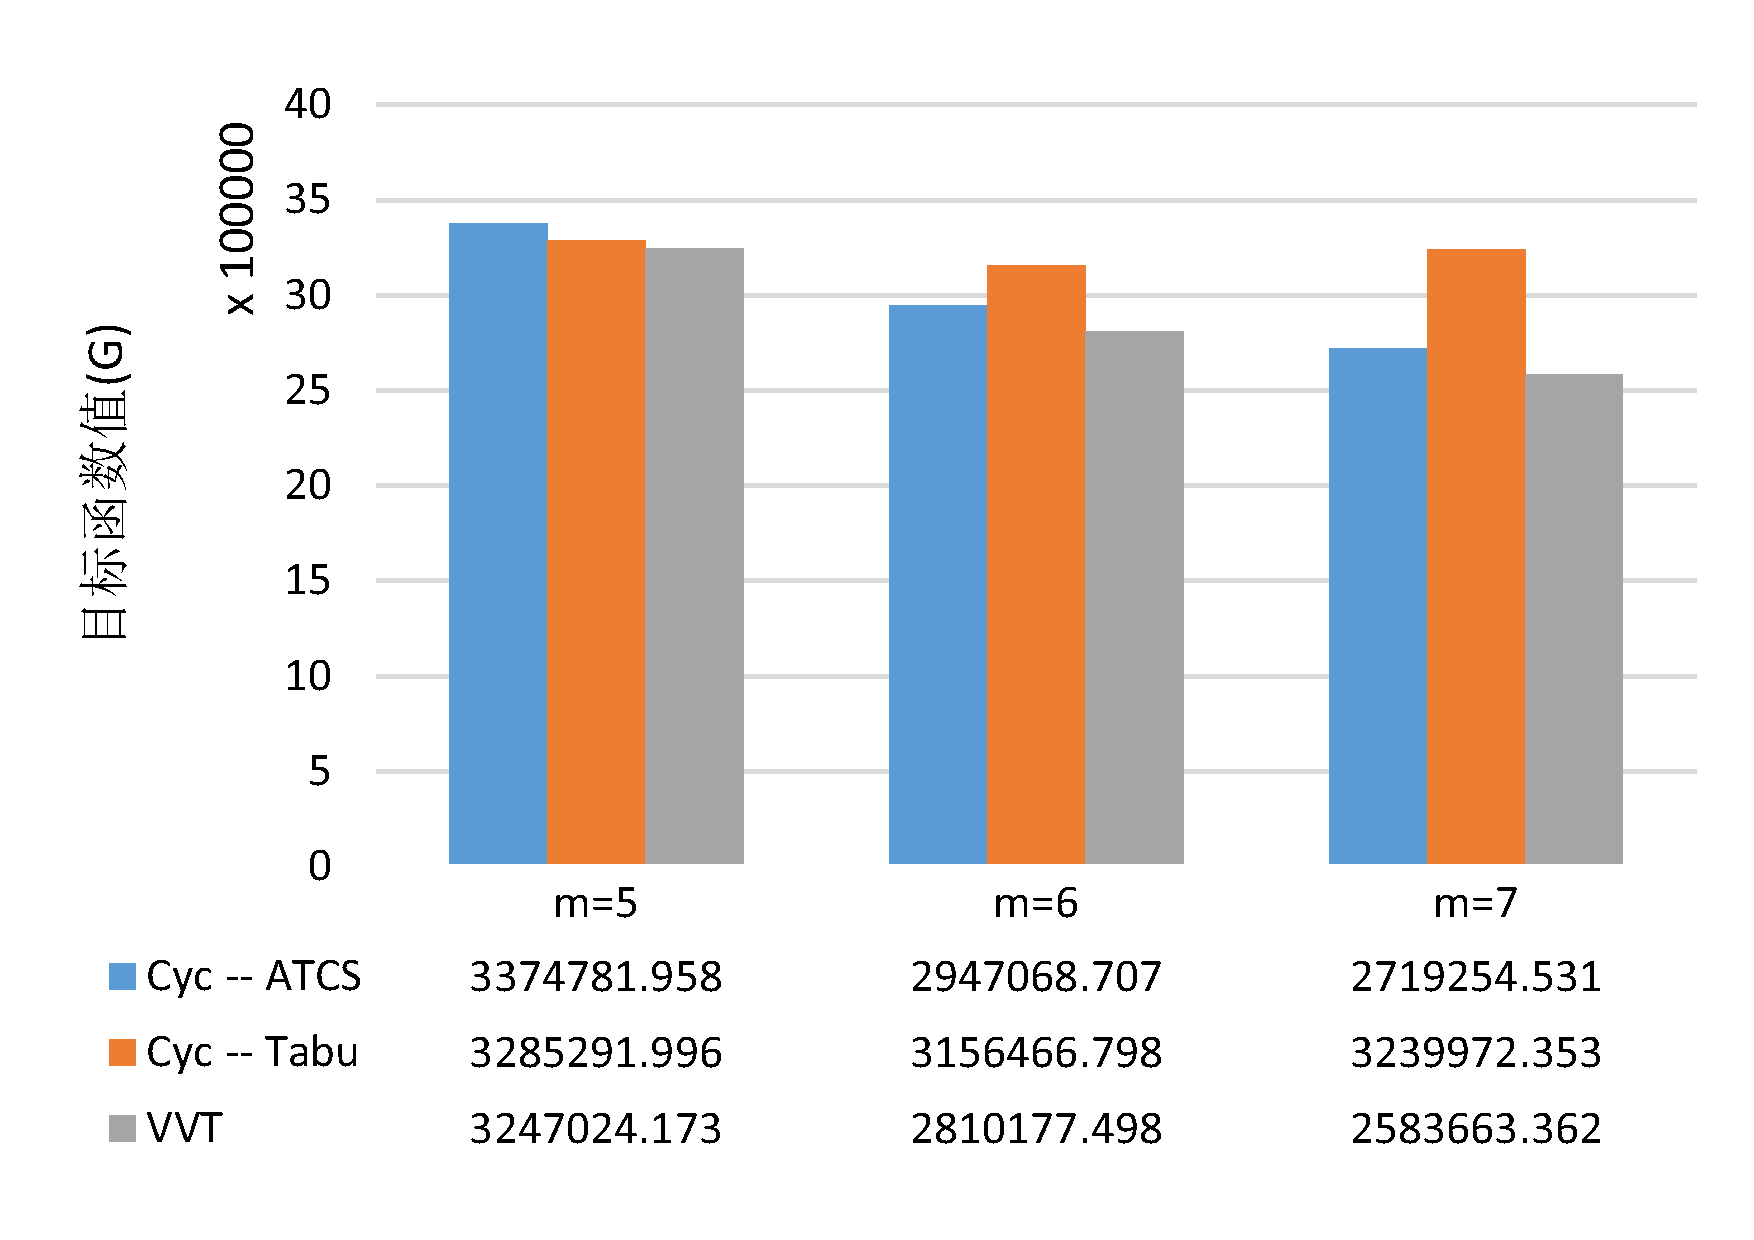
\includegraphics[height = 6cm, angle = -90]{continue_04_500}}
\subfloat[$n = 750$]{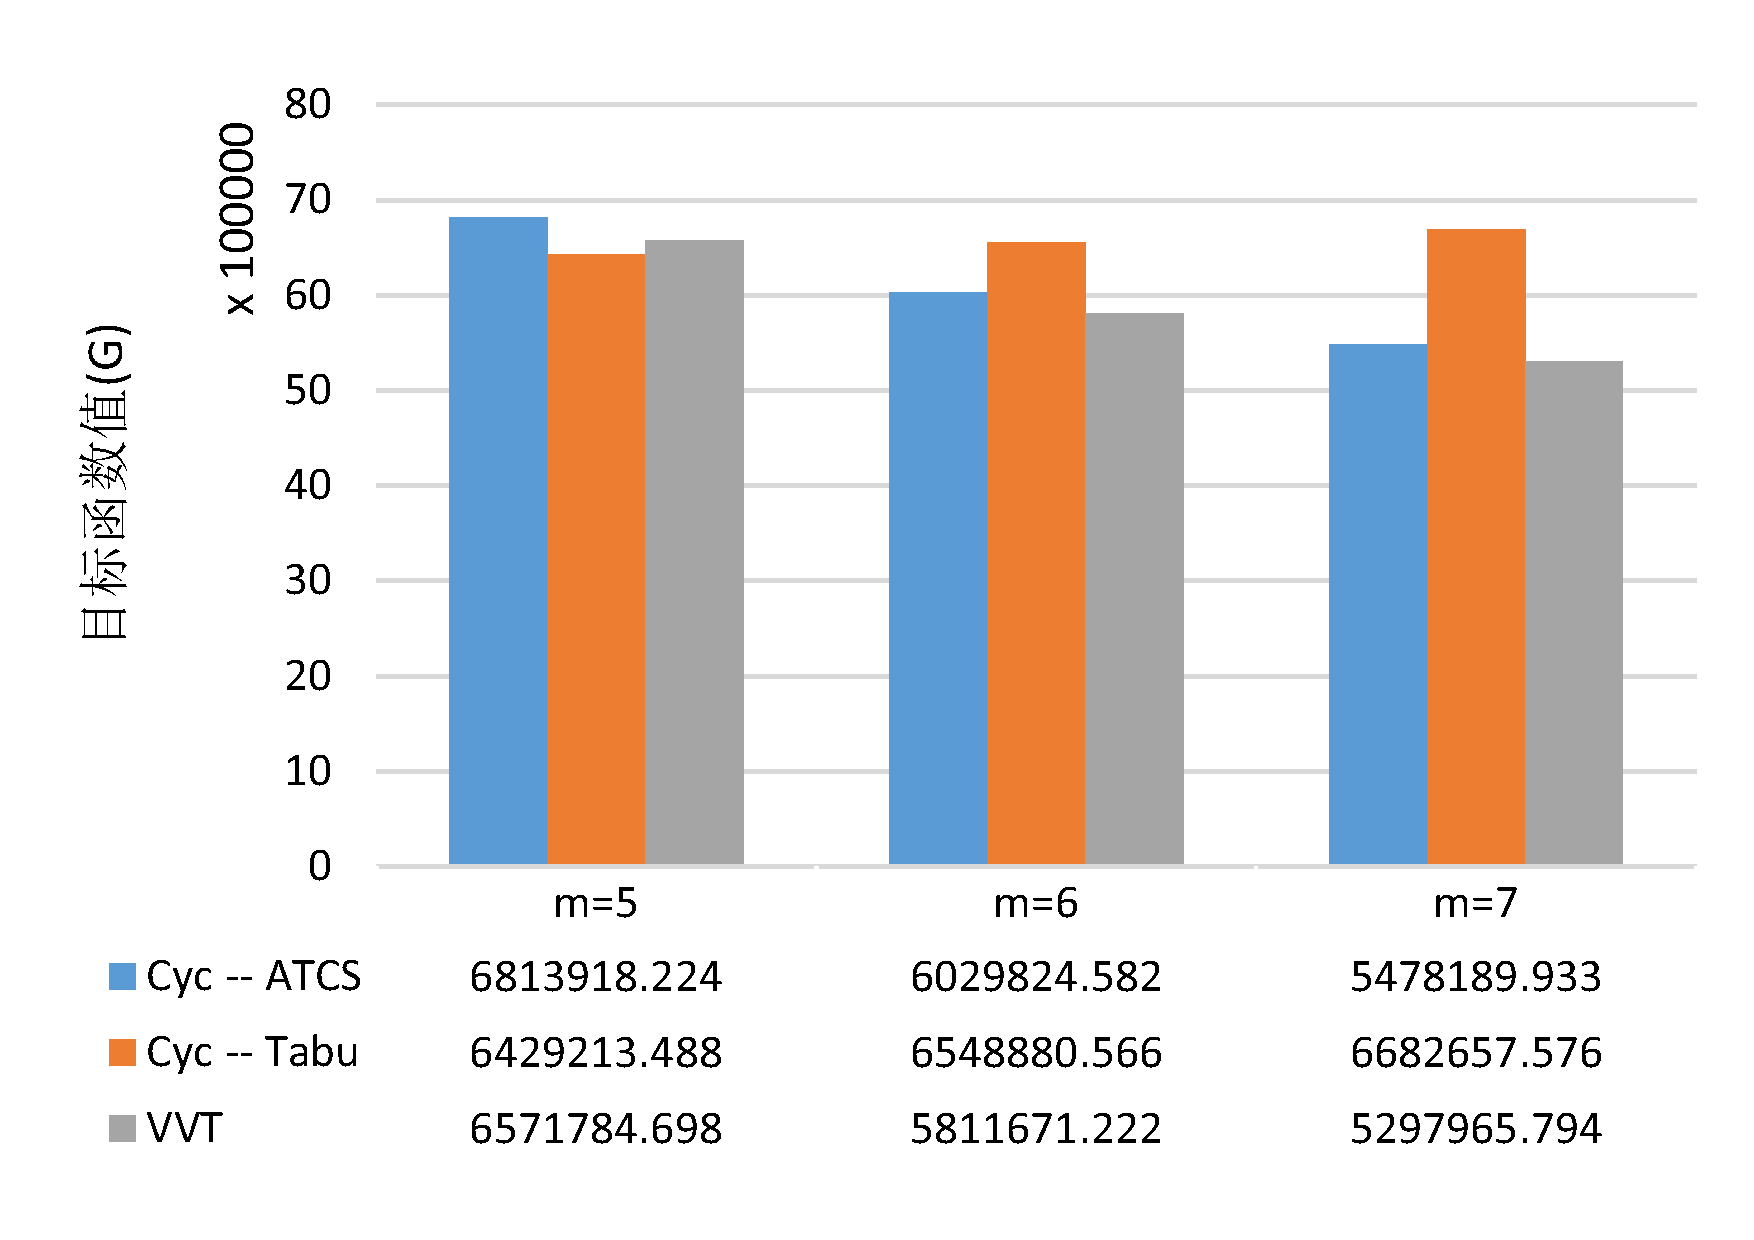
\includegraphics[height = 6cm, angle = -90]{continue_04_750}}
\subfloat[$n = 1000$]{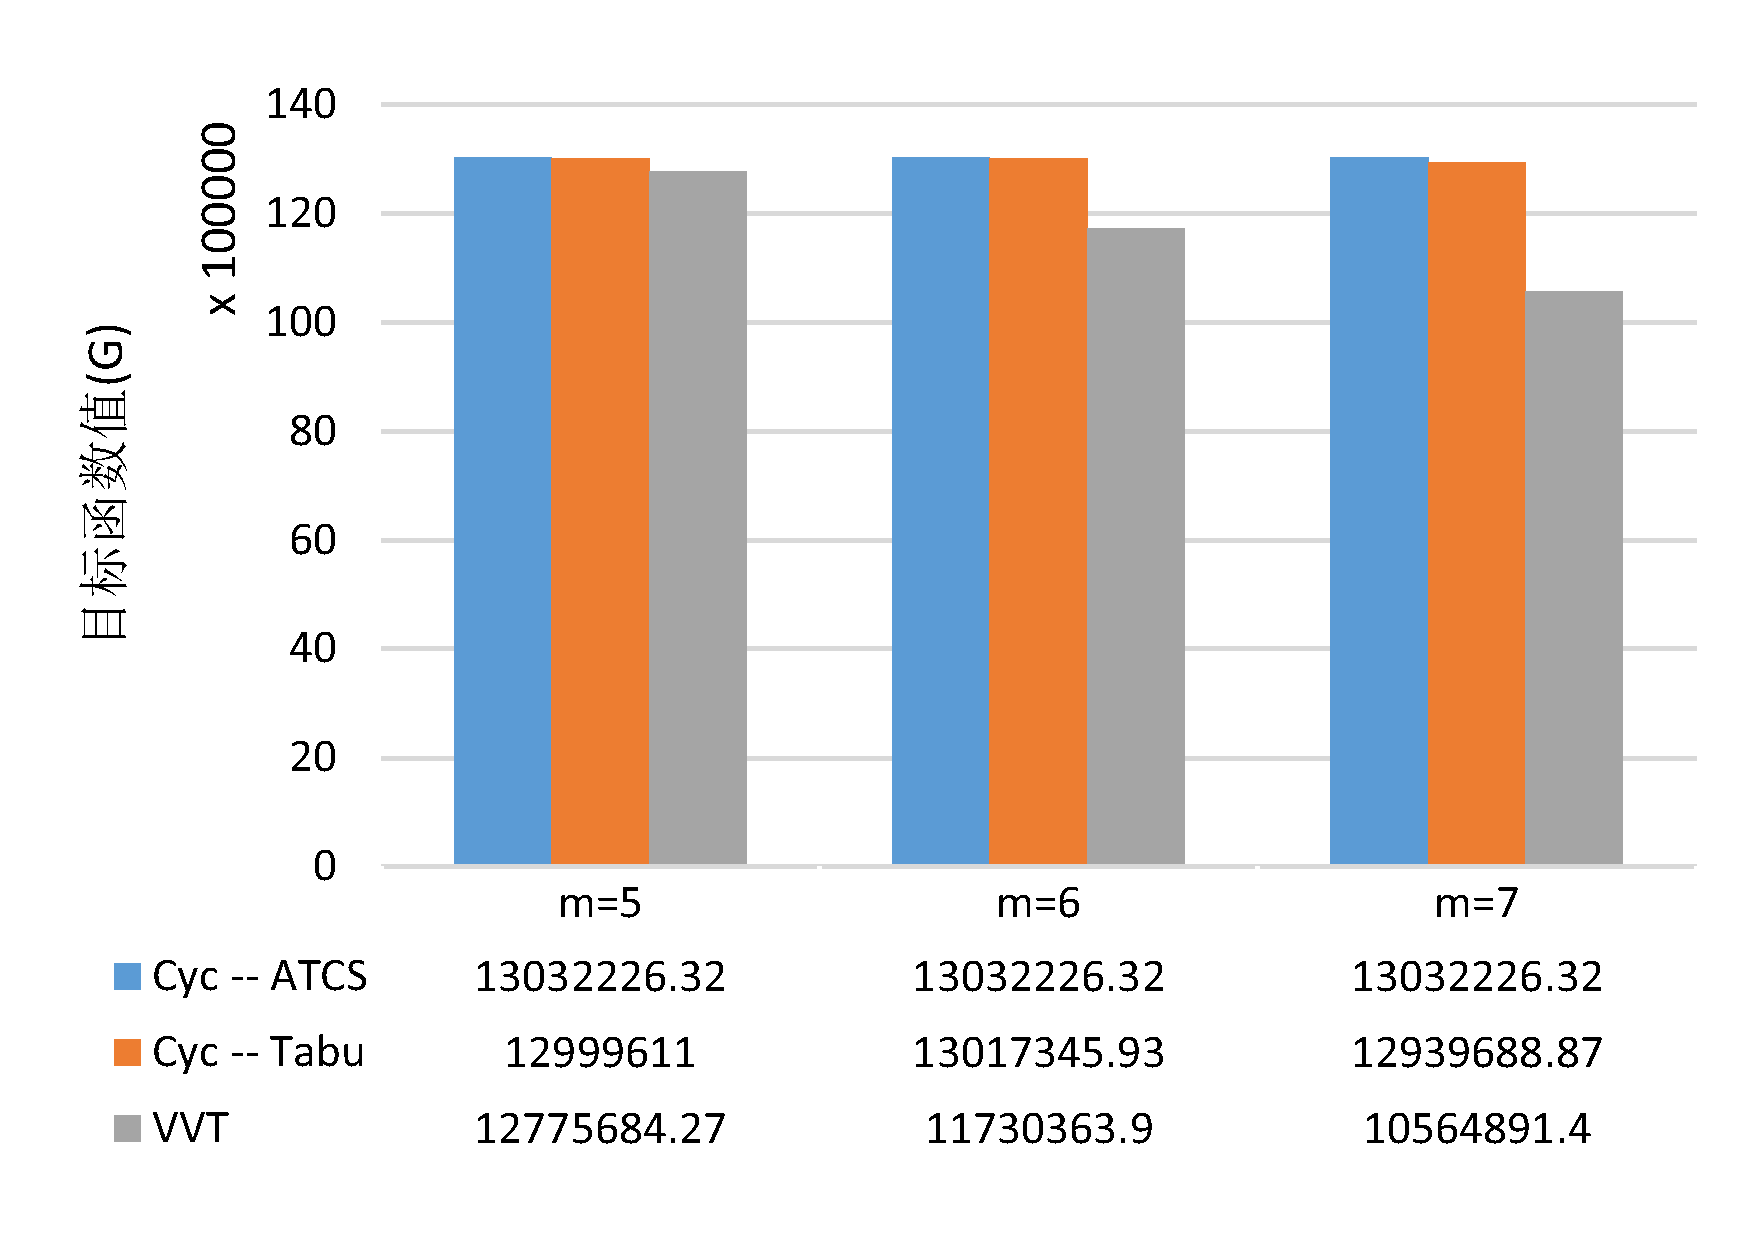
\includegraphics[height = 6cm, angle = -90]{continue_04_1000}}
\caption{\label{fig:result4}模型$2$的Cyc -- ATCS、Cyc -- Tabu、VVT 算法求解目标函数值比较$(\lambda_1 = 0.4)$}
\end{sidewaysfigure}

\begin{sidewaysfigure}
\centering
\subfloat[$n = 20$]{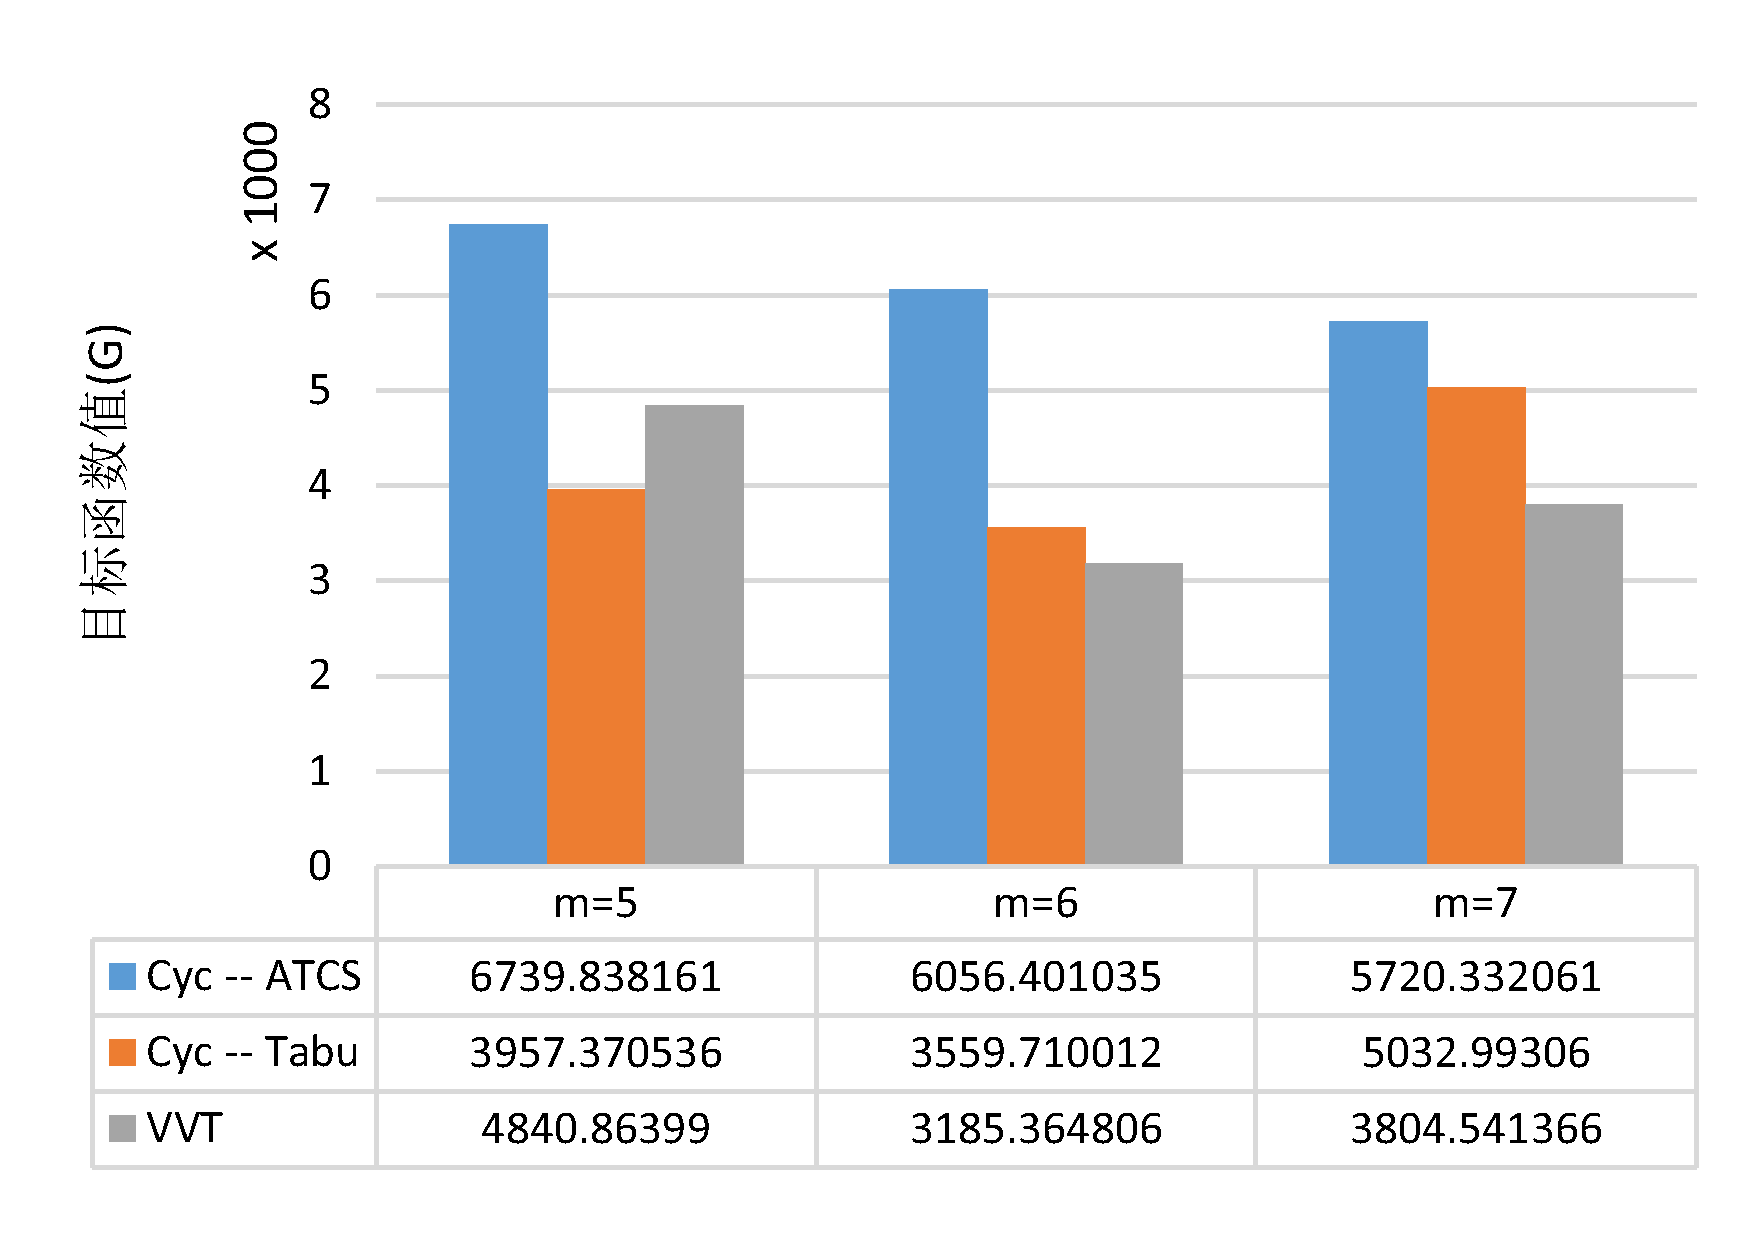
\includegraphics[height = 6cm, angle = -90]{continue_05_20}}
\subfloat[$n = 30$]{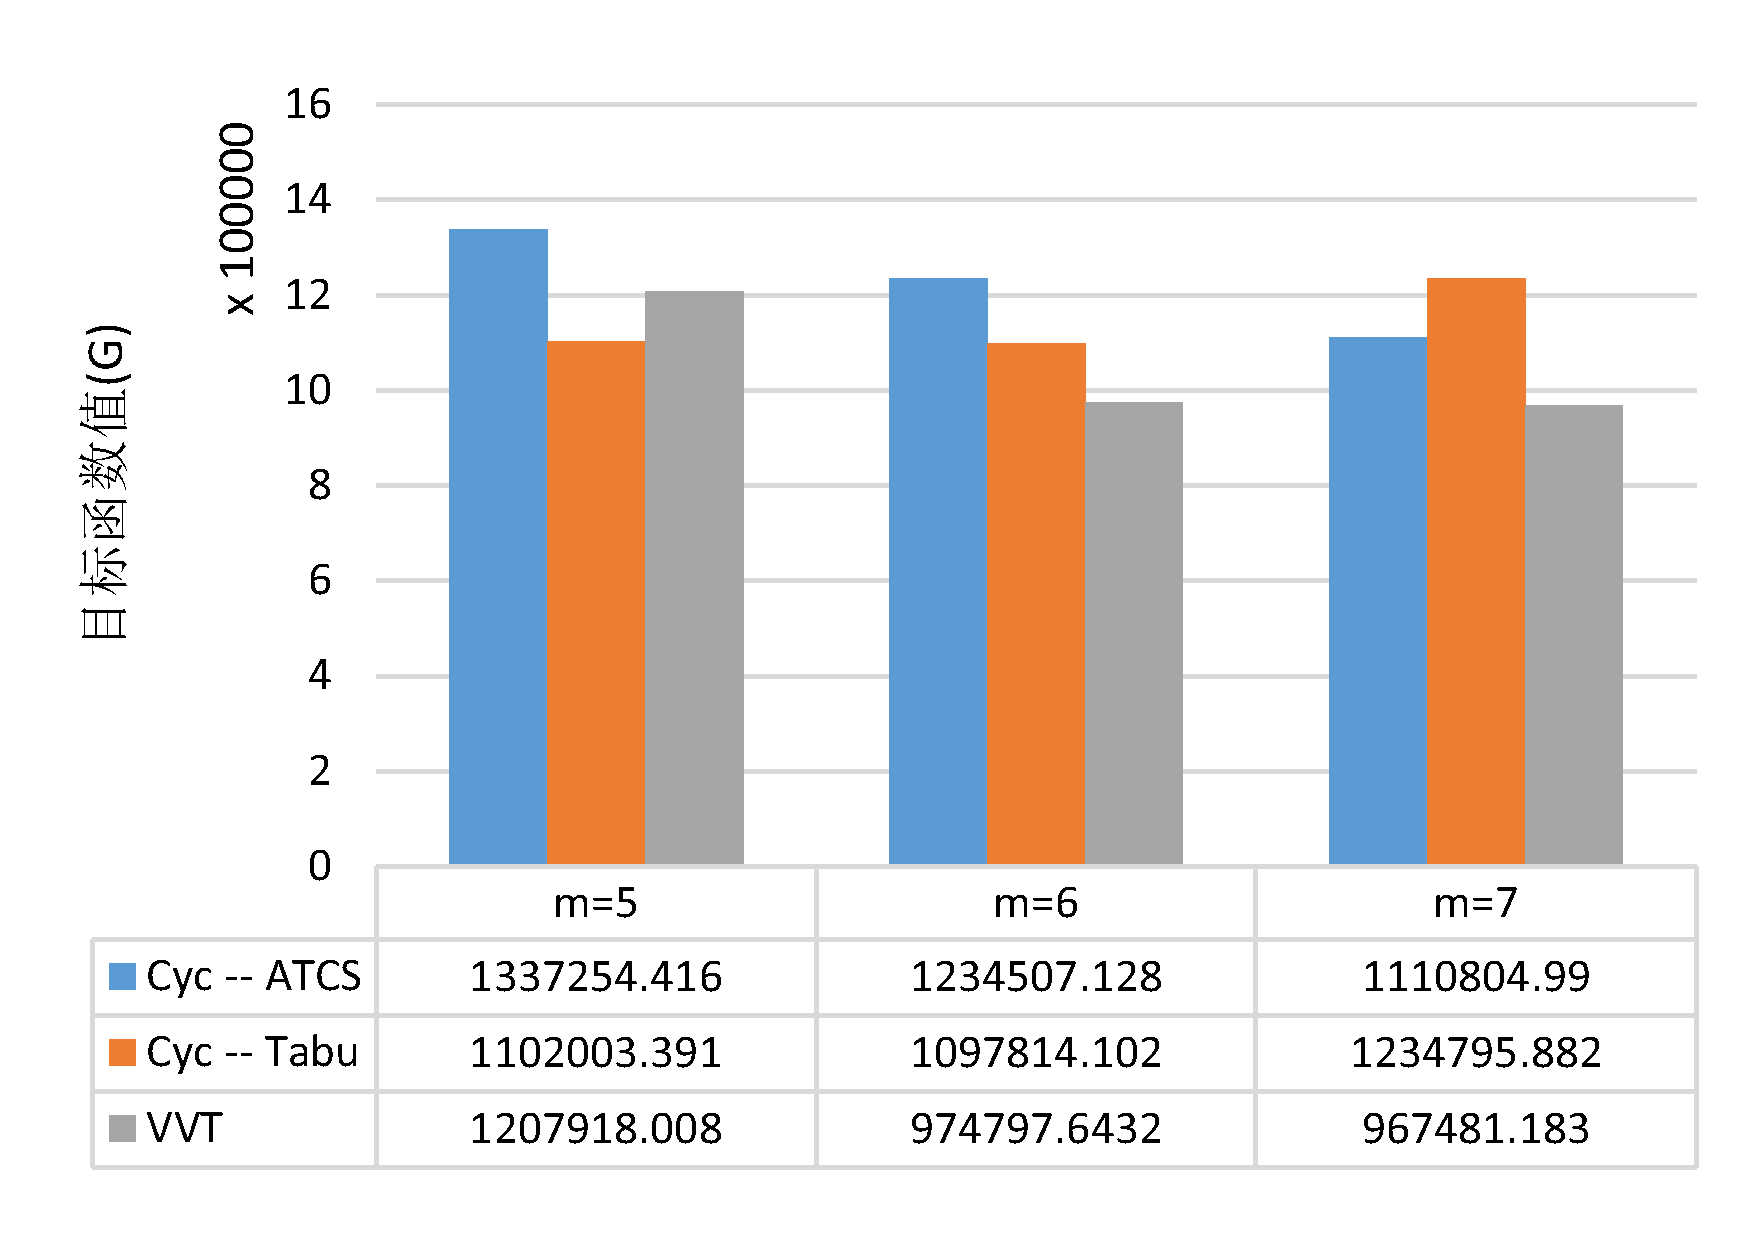
\includegraphics[height = 6cm, angle = -90]{continue_05_300}}
\subfloat[$n = 50$]{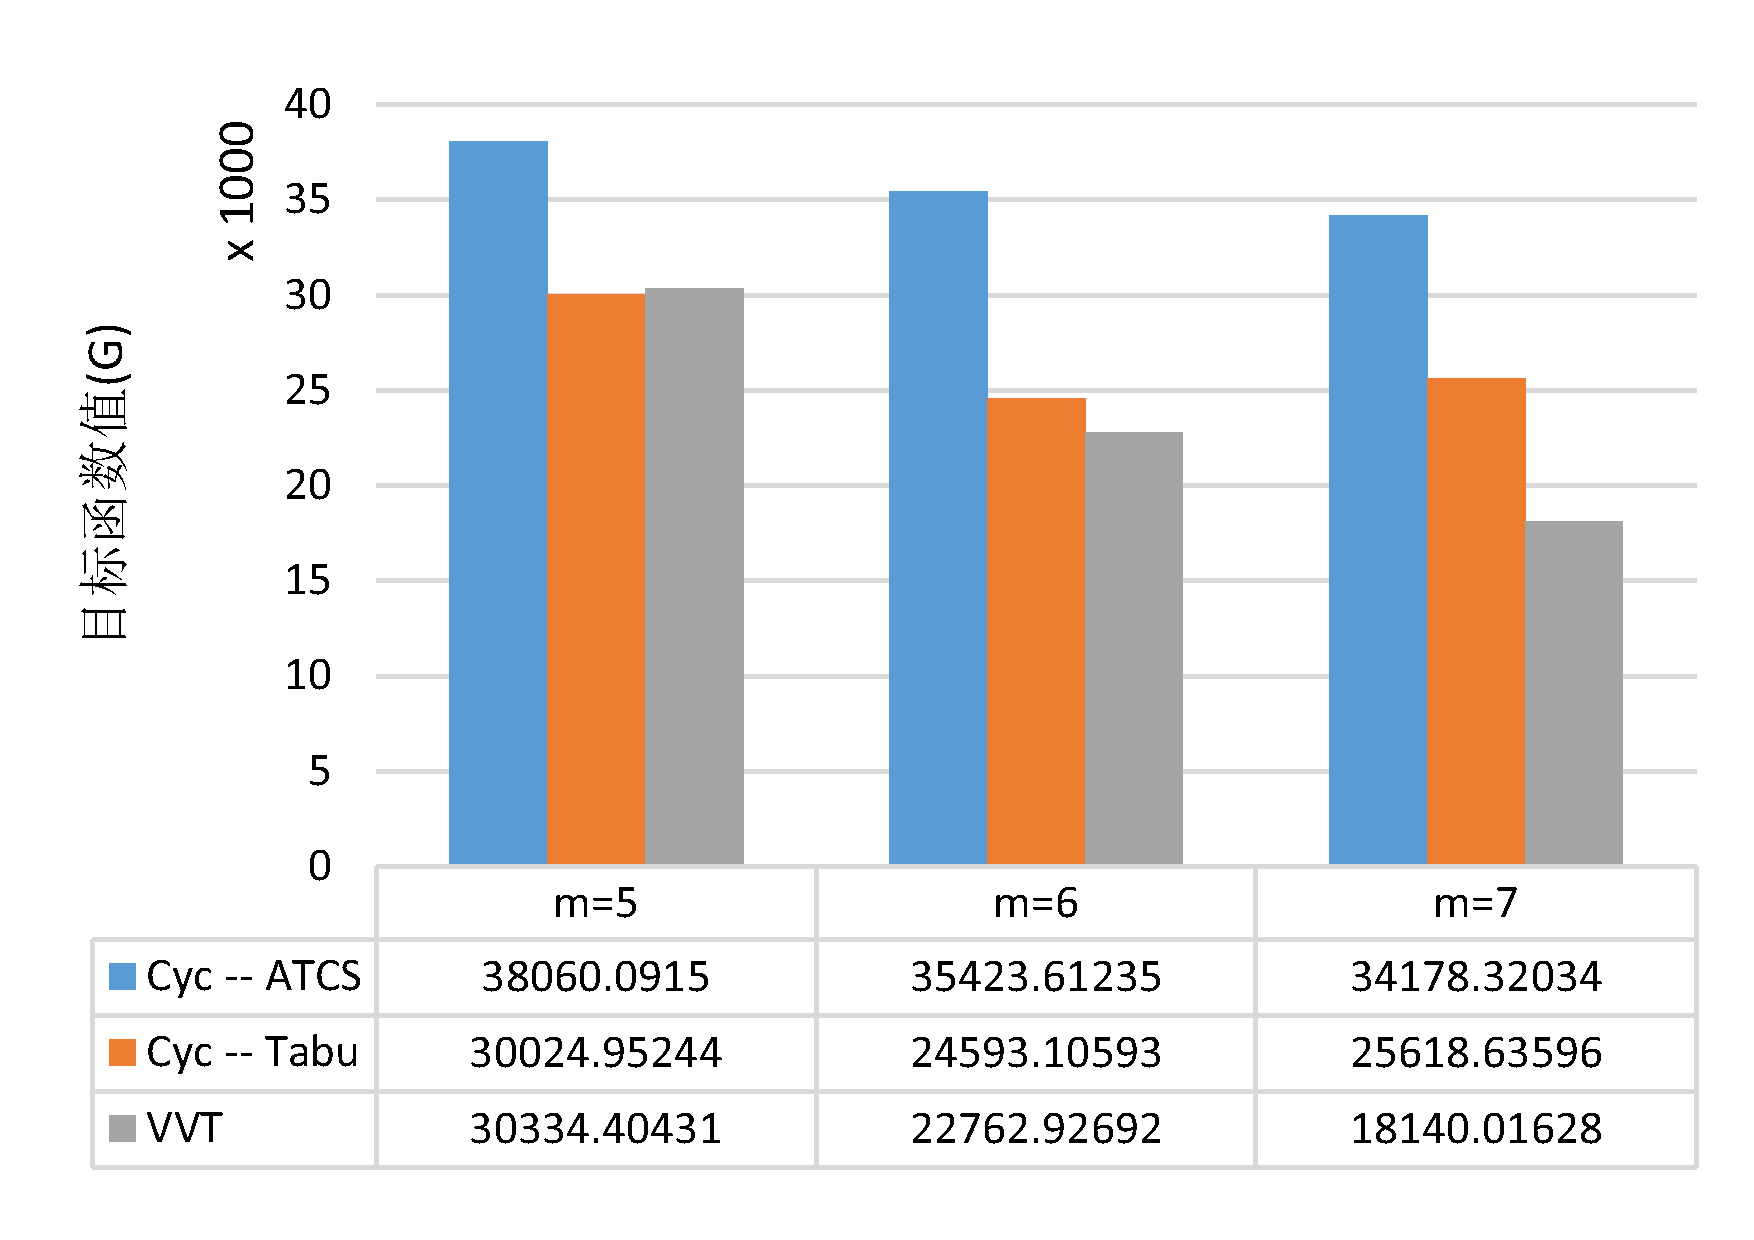
\includegraphics[height = 6cm, angle = -90]{continue_05_50}}
\subfloat[$n = 70$]{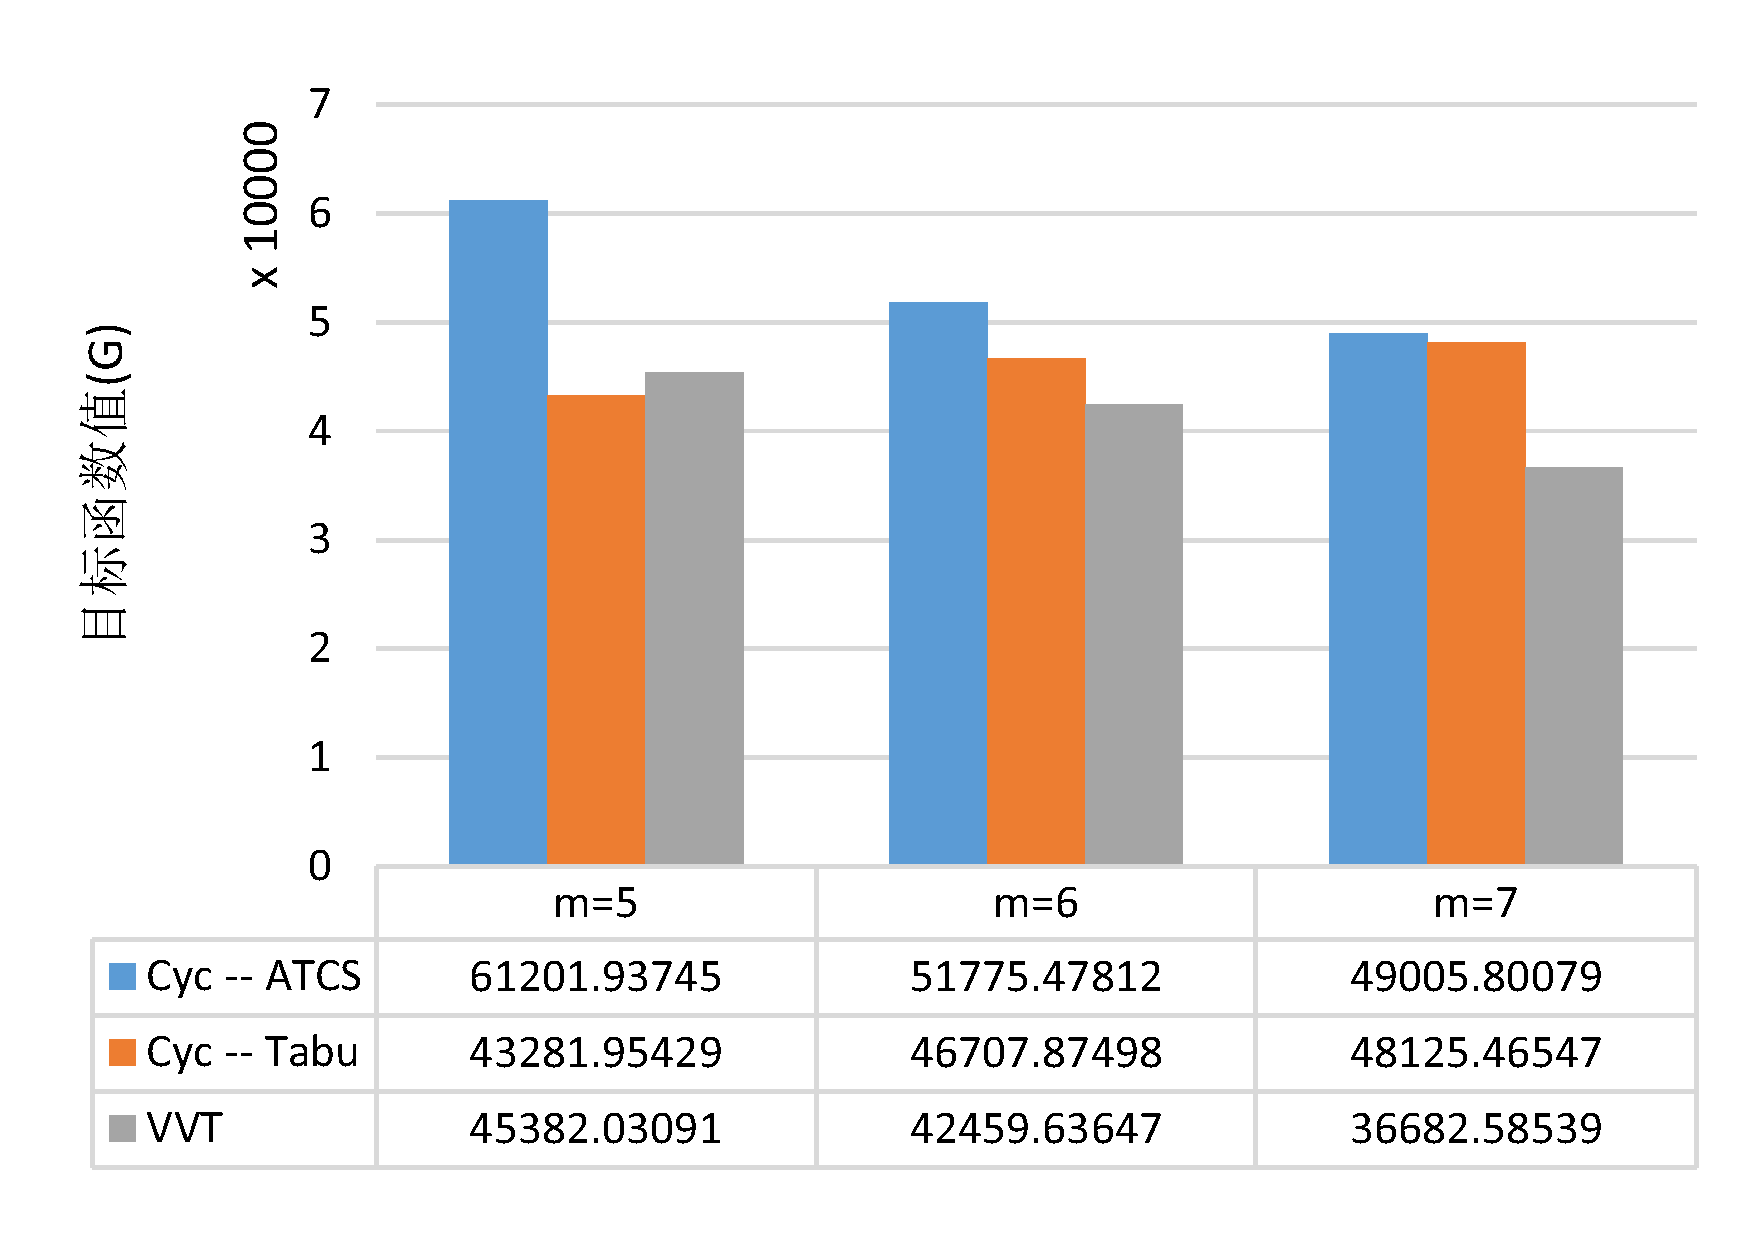
\includegraphics[height = 6cm, angle = -90]{continue_05_70}}\\
\subfloat[$n = 100$]{\includegraphics[height = 6cm, angle = -90]{continue_05_100}}
\subfloat[$n = 150$]{\includegraphics[height = 6cm, angle = -90]{continue_05_150}}
\subfloat[$n = 200$]{\includegraphics[height = 6cm, angle = -90]{continue_05_200}}
\subfloat[$n = 300$]{\includegraphics[height = 6cm, angle = -90]{continue_05_300}}\\
\subfloat[$n = 500$]{\includegraphics[height = 6cm, angle = -90]{continue_05_500}}
\subfloat[$n = 750$]{\includegraphics[height = 6cm, angle = -90]{continue_05_750}}
\subfloat[$n = 1000$]{\includegraphics[height = 6cm, angle = -90]{continue_05_1000}}
\caption{\label{fig:result5}模型$2$的Cyc -- ATCS、Cyc -- Tabu、VVT 算法求解目标函数值比较$(\lambda_1 = 0.5)$}
\end{sidewaysfigure}

\begin{sidewaysfigure}
\centering
\subfloat[$n = 20$]{\includegraphics[height = 6cm, angle = -90]{continue_06_20}}
\subfloat[$n = 30$]{\includegraphics[height = 6cm, angle = -90]{continue_06_300}}
\subfloat[$n = 50$]{\includegraphics[height = 6cm, angle = -90]{continue_06_50}}
\subfloat[$n = 70$]{\includegraphics[height = 6cm, angle = -90]{continue_06_70}}\\
\subfloat[$n = 100$]{\includegraphics[height = 6cm, angle = -90]{continue_06_100}}
\subfloat[$n = 150$]{\includegraphics[height = 6cm, angle = -90]{continue_06_150}}
\subfloat[$n = 200$]{\includegraphics[height = 6cm, angle = -90]{continue_06_200}}
\subfloat[$n = 300$]{\includegraphics[height = 6cm, angle = -90]{continue_06_300}}\\
\subfloat[$n = 500$]{\includegraphics[height = 6cm, angle = -90]{continue_06_500}}
\subfloat[$n = 750$]{\includegraphics[height = 6cm, angle = -90]{continue_06_750}}
\subfloat[$n = 1000$]{\includegraphics[height = 6cm, angle = -90]{continue_06_1000}}
\caption{\label{fig:result6}模型$2$的Cyc -- ATCS、Cyc -- Tabu、VVT 算法求解目标函数值比较$(\lambda_1 = 0.6)$}
\end{sidewaysfigure}

\begin{sidewaysfigure}
\centering
\subfloat[$n = 20$]{\includegraphics[height = 6cm, angle = -90]{Rb_04_20}}
\subfloat[$n = 30$]{\includegraphics[height = 6cm, angle = -90]{Rb_04_300}}
\subfloat[$n = 50$]{\includegraphics[height = 6cm, angle = -90]{Rb_04_50}}
\subfloat[$n = 70$]{\includegraphics[height = 6cm, angle = -90]{Rb_04_70}}\\
\subfloat[$n = 100$]{\includegraphics[height = 6cm, angle = -90]{Rb_04_100}}
\subfloat[$n = 150$]{\includegraphics[height = 6cm, angle = -90]{Rb_04_150}}
\subfloat[$n = 200$]{\includegraphics[height = 6cm, angle = -90]{Rb_04_200}}
\subfloat[$n = 300$]{\includegraphics[height = 6cm, angle = -90]{Rb_04_300}}\\
\subfloat[$n = 500$]{\includegraphics[height = 6cm, angle = -90]{Rb_04_500}}
\subfloat[$n = 750$]{\includegraphics[height = 6cm, angle = -90]{Rb_04_750}}
\subfloat[$n = 1000$]{\includegraphics[height = 6cm, angle = -90]{Rb_04_1000}}
\caption{\label{fig:result7}模型$2$的Cyc -- ATCS、Cyc -- Tabu、VVT 算法求解流水线均衡率比较$(\lambda_1 = 0.4)$}
\end{sidewaysfigure}

\begin{sidewaysfigure}
\centering
\subfloat[$n = 20$]{\includegraphics[height = 6cm, angle = -90]{Rb_05_20}}
\subfloat[$n = 30$]{\includegraphics[height = 6cm, angle = -90]{Rb_05_300}}
\subfloat[$n = 50$]{\includegraphics[height = 6cm, angle = -90]{Rb_05_50}}
\subfloat[$n = 70$]{\includegraphics[height = 6cm, angle = -90]{Rb_05_70}}\\
\subfloat[$n = 100$]{\includegraphics[height = 6cm, angle = -90]{Rb_05_100}}
\subfloat[$n = 150$]{\includegraphics[height = 6cm, angle = -90]{Rb_05_150}}
\subfloat[$n = 200$]{\includegraphics[height = 6cm, angle = -90]{Rb_05_200}}
\subfloat[$n = 300$]{\includegraphics[height = 6cm, angle = -90]{Rb_05_300}}\\
\subfloat[$n = 500$]{\includegraphics[height = 6cm, angle = -90]{Rb_05_500}}
\subfloat[$n = 750$]{\includegraphics[height = 6cm, angle = -90]{Rb_05_750}}
\subfloat[$n = 1000$]{\includegraphics[height = 6cm, angle = -90]{Rb_05_1000}}
\caption{\label{fig:result8}模型$2$的Cyc -- ATCS、Cyc -- Tabu、VVT 算法求解流水线均衡率比较$(\lambda_1 = 0.5)$}
\end{sidewaysfigure}

\begin{sidewaysfigure}
\centering
\subfloat[$n = 20$]{\includegraphics[height = 6cm, angle = -90]{Rb_06_20}}
\subfloat[$n = 30$]{\includegraphics[height = 6cm, angle = -90]{Rb_06_300}}
\subfloat[$n = 50$]{\includegraphics[height = 6cm, angle = -90]{Rb_06_50}}
\subfloat[$n = 70$]{\includegraphics[height = 6cm, angle = -90]{Rb_06_70}}\\
\subfloat[$n = 100$]{\includegraphics[height = 6cm, angle = -90]{Rb_06_100}}
\subfloat[$n = 150$]{\includegraphics[height = 6cm, angle = -90]{Rb_06_150}}
\subfloat[$n = 200$]{\includegraphics[height = 6cm, angle = -90]{Rb_06_200}}
\subfloat[$n = 300$]{\includegraphics[height = 6cm, angle = -90]{Rb_06_300}}\\
\subfloat[$n = 500$]{\includegraphics[height = 6cm, angle = -90]{Rb_06_500}}
\subfloat[$n = 750$]{\includegraphics[height = 6cm, angle = -90]{Rb_06_750}}
\subfloat[$n = 1000$]{\includegraphics[height = 6cm, angle = -90]{Rb_06_1000}}
\caption{\label{fig:result9}模型$2$的Cyc -- ATCS、Cyc -- Tabu、VVT 算法求解流水线均衡率比较$(\lambda_1 = 0.6)$}
\end{sidewaysfigure}
\chapter{算法代码}
\begin{asparaenum}
\item experiment\_data.py
\end{asparaenum}
\lstset{	basicstyle = \tiny\ttfamily,
	keywordstyle = \color{blue}\bfseries,
	stringstyle = \color{red},
	emph = {solve},
	emphstyle = \color{Green}\bfseries,
	commentstyle = \color{CadetBlue}
	}
\begin{lstlisting}[language = Python]
import sys
sys.path.append(".\\functions")
import generate
from collections import namedtuple
Item = namedtuple("Item", ['process','due','wt','wc'])

def  h(lambda1,lambda2,tardiness,completion,wt,wc):			# define the contribution of one item for the obj function
	value = lambda1*wt*tardiness + lambda2*wc*completion
	return value

def solve(input_data):
	Data = input_data.split('\n')					# load data
	n = len(Data) -1						# get the amount of items
	print n
	items = []
	for j in xrange(n):
		data = Data[j]
		parts = data.split()
		p = int(parts[0])					# get the process time
		s = int(parts[2])						# get the setup time
		d = int(parts[3])					# get the due date
		wt = int(parts[4])					# get the tardiness weights
		wc = int(parts[5])					# get the completion weights
		items.append(Item(p+s,d,wt,wc))			# combine those item data
	print 'Data loaded!'
	J = range(n)
	m = 5
	S = []
	a = []
	tl = []
	L = []
	c = [None]*n
	for l in xrange(m):
		S.append([])
		a.append(0)
		tl.append(0)
	t = 0
	f = open(".\\result\\sky",'w')
	while J:
		if 0 in a:
			l_star = a.index(0)
			p,d,wt = [],[],[]
			for j in J:				
				item = items[j]
				p.append(item.process)
				d.append(item.due)
				wt.append(item.wt)
			orderidx = generate.Idx(t,p,d,wt)
			j_star = J[orderidx.index(max(orderidx))]
			S[l_star].append(j_star)
			J.remove(j_star)
			L.append(j_star)
			tl[l_star] = t + items[j_star].process
			c[j_star] = tl[l_star]
			a[l_star] = 1
		else:
			t_star = min(tl)
			for l in xrange(m):
				if tl[l] == t_star:
					a[l] = 0
			t = t_star
	print 'initial sloution done!'
	f.write(str(S) + '\n' + str(L) + '\n' + str(c))
	f.close()


import sys
if __name__ == '__main__':
	if len(sys.argv) > 1:
		file_location = sys.argv[1].strip()
#		output = sys.argv[2].strip()
		input_data_file = open(file_location, 'r')
		input_data = ''.join(input_data_file.readlines())
		input_data_file.close()
		solve(input_data)
\end{lstlisting}
\section{456456}
\addcontentsline{toc}{section}{附录1 毕业设计文献综述}
\addcontentsline{toc}{section}{附录2 毕业设计开题报告}
\addcontentsline{toc}{section}{附录3 毕业设计外文翻译(中文译文与外文原文)}
\hspace*{7.0mm}
\hspace*{4.0mm}
\begin{minipage}[t]{95mm}
    \songti\bfseries{
    \sectionmark{附录1 毕业设计文献综述}
    附录1 毕业设计文献综述

    \vspace*{7.0mm}

    \sectionmark{附录2 毕业设计开题报告}
    附录2 毕业设计开题报告

    \vspace*{7.0mm}

    \sectionmark{附录3 毕业设计外文翻译(中文译文与外文原文)}
    附录3 毕业设计外文翻译(中文译文与外文原文)}
\end{minipage}
            % 附录

\end{document}                                  % 结束全文
